\chapter{Análisis Global de datos Meteorológicos}
\section{Análisis Univariado}

\subsection{Estadisticas Descriptivas Globales}

\begin{table}[H]
\centering
\caption{Global descriptive statistics of meteorological variables}
\label{tab:global_statistics}
\small
\begin{tabular}{lrrrrr}
\toprule
\textbf{Statistic} & \textbf{P (mm)} & \textbf{RH (\%)} & \textbf{T (°C)} & \textbf{WS (m/s)} & \textbf{PET (mm)} \\
\midrule
$n$                         & 12312 & 12312 & 12312 & 12312 & 12312 \\
Minimum                    & 0.00   & 21.67  & -1.41  & 0.00   & 2.9991 \\
1st Quartile               & 0.00   & 58.63  & 9.95   & 1.90   & 5.0882 \\
Median                     & 4.80   & 69.66  & 12.08  & 2.60   & 5.6153 \\
Mean                       & 34.82  & 68.19  & 13.06  & 2.88   & 5.7215 \\
3rd Quartile               & 51.00  & 79.11  & 16.54  & 3.50   & 6.4799 \\
Maximum                    & 424.10 & 99.62  & 26.52  & 27.80  & 9.0703 \\
Range                      & 424.10 & 77.95  & 27.93  & 27.80  & 6.0712 \\
Interquartile Range        & 51.00  & 20.30  & 6.59   & 1.60   & 1.3917 \\
Variance                   & 3020.50 & 195.25 & 24.25  & 2.4378 & 1.0611 \\
Standard Deviation         & 54.96  & 13.97  & 4.92   & 1.56   & 1.0301 \\
Coefficient of Variation   & 1.58   & 0.20   & 0.38   & 0.54   & 0.18 \\
Skewness                 & 1.97   & -0.44  & 0.25   & 2.56   & 0.15 \\
Kurtosis                   & 4.06   & -0.53  & -0.18  & 19.76  & -0.19 \\
\bottomrule
\end{tabular}
\end{table}


La Tabla~\ref{tab:global_statistics} muestra las estadísticas descriptivas globales de las variables meteorológicas. La precipitación (P) presenta una distribución altamente asimétrica a la derecha, con una Media considerablemente mayor que la Mediana y un Rango amplio, lo que evidencia eventos extremos de lluvia. La humedad relativa (RH) muestra una distribución relativamente simétrica, con valores concentrados entre 60~\% y 90~\%, y baja variabilidad. La temperatura (T) exhibe una distribución cercana a la simetría, con una Media de 13.06~$^\circ$C y una dispersión moderada. La velocidad del viento (WS) tiene una alta Skewness positiva y curtosis, lo que sugiere la presencia de ráfagas fuertes poco frecuentes. Por último, la evapotranspiración potencial (PET) muestra una distribución bastante estable, con baja variabilidad y similitud entre Media y mediana, indicando homogeneidad en los valores registrados.

\subsubsection*{Precipitación (P)}

\begin{figure}[H]
    \caption{Histograma de la Precipitación (P).}
    \centering
    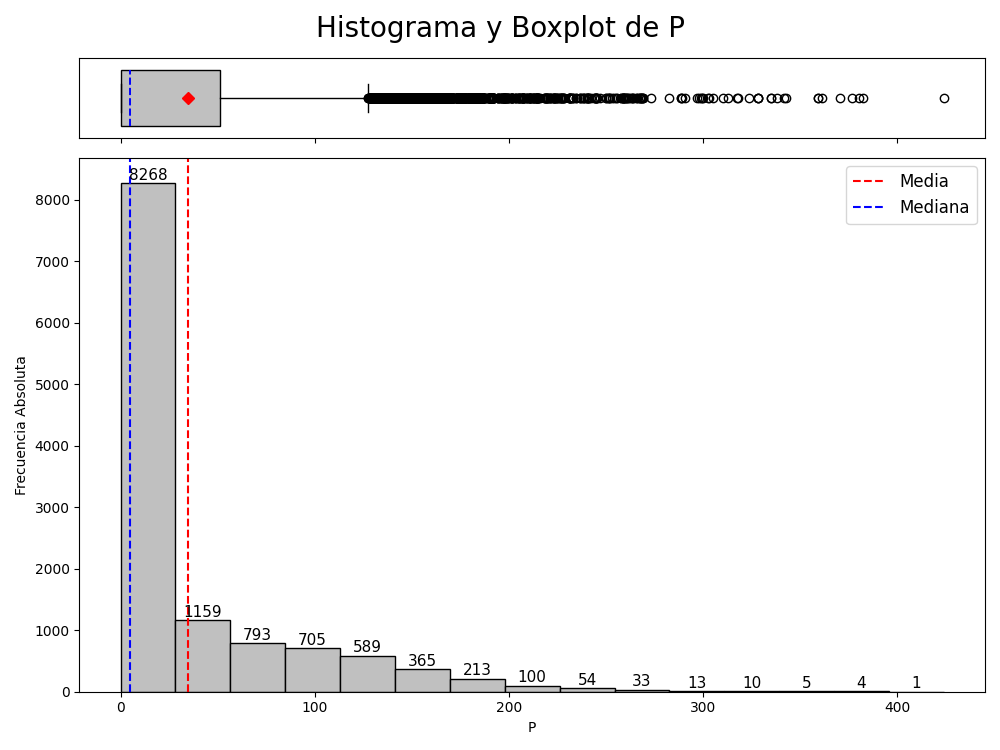
\includegraphics[width=0.4\textwidth]{resultados/global/univariado/P_histograma.png}
    \label{fig:P_histograma}
\end{figure}

La distribución de la precipitación es altamente asimétrica a la derecha. Se observa un gran número de valores atípicos superiores, reflejo de eventos de lluvia extrema. La Media supera considerablemente a la mediana, lo que confirma esta asimetría. La mayoría de los registros se concentran por debajo de \SI{50}{\milli\meter}.

\vspace{2em}

\subsubsection*{Temperatura (T)}

\begin{figure}[H]
    \caption{Histograma de la Temperatura (T).}
    \centering
    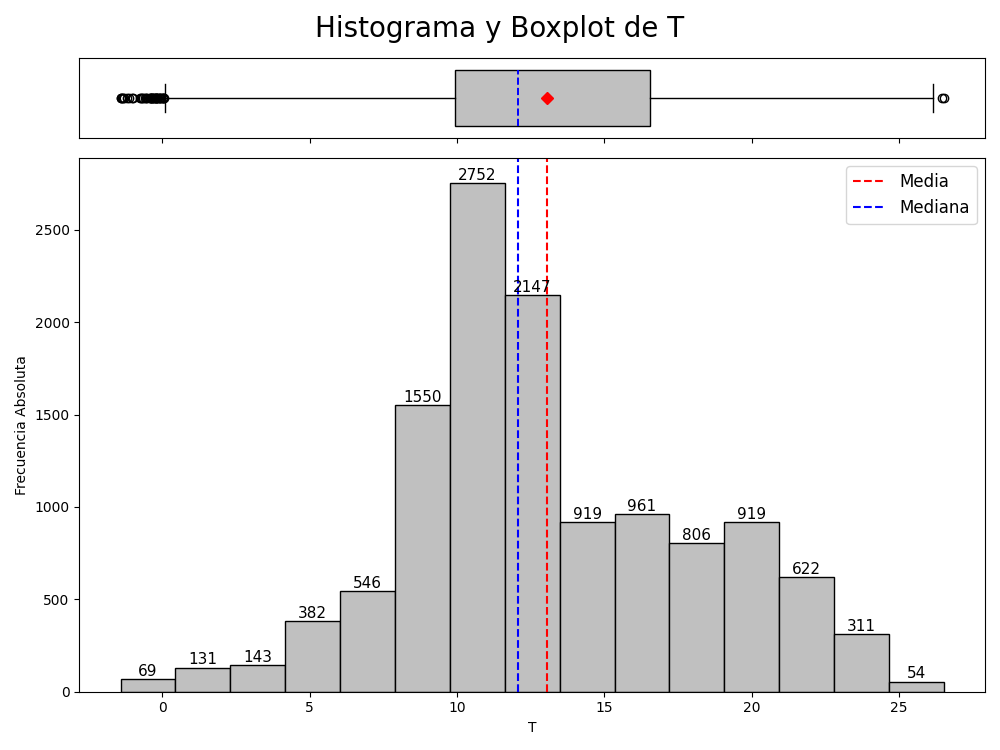
\includegraphics[width=0.4\textwidth]{resultados/global/univariado/T_histograma.png}
    \label{fig:T_histograma}
\end{figure}

La temperatura presenta una distribución aproximadamente simétrica, con algunos valores atípicos en ambos extremos. La Media y la Mediana son cercanas, lo que sugiere un equilibrio en la dispersión. La mayoría de los valores se encuentran entre \SI{10}{\degreeCelsius} y \SI{20}{\degreeCelsius}.

\newpage

\subsubsection*{Humedad Relativa (RH)}

\begin{figure}[H]
    \caption{Histograma de la Humedad Relativa (RH).}
    \centering
    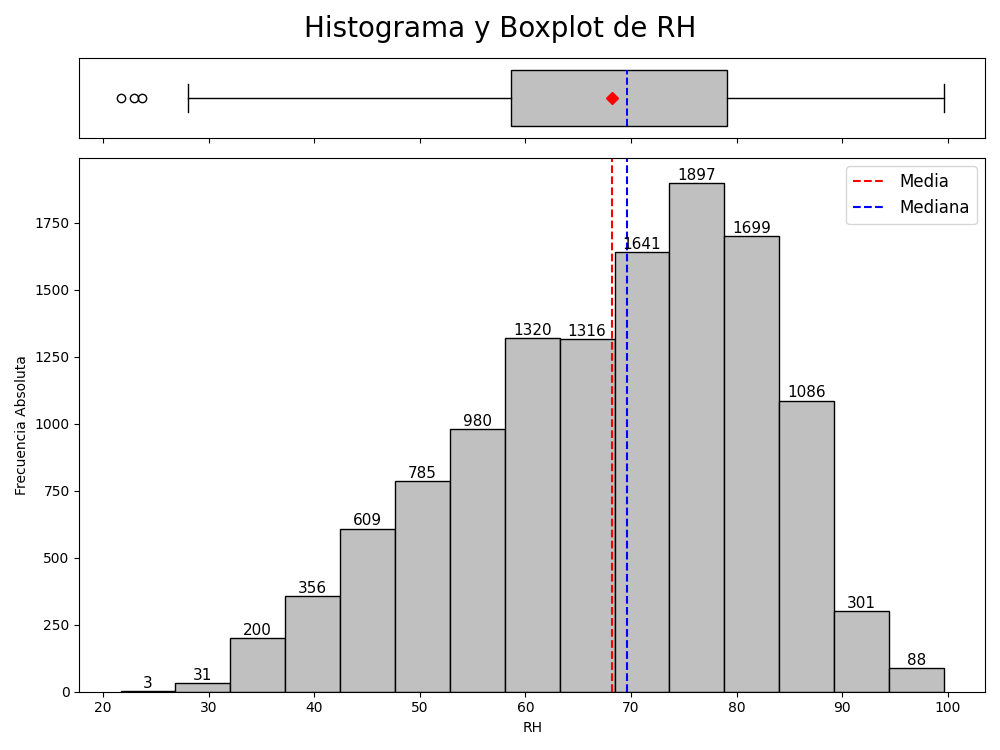
\includegraphics[width=0.4\textwidth]{resultados/global/univariado/RH_histograma.png}
    \label{fig:RH_histograma}
\end{figure}

La humedad relativa muestra una distribución sesgada hacia la izquierda, concentrando la mayor parte de los valores entre \SI{60}{\percent} y \SI{90}{\percent}. Algunos valores atípicos inferiores podrían asociarse a las estaciones que presentan condiciones secas excepcionales. La Mediana es ligeramente mayor que la media.

\vspace{2em}

\subsubsection*{Velocidad del Viento (WS)}

\begin{figure}[H]
    \caption{Histograma de la Velocidad del Viento (WS).}
    \centering
    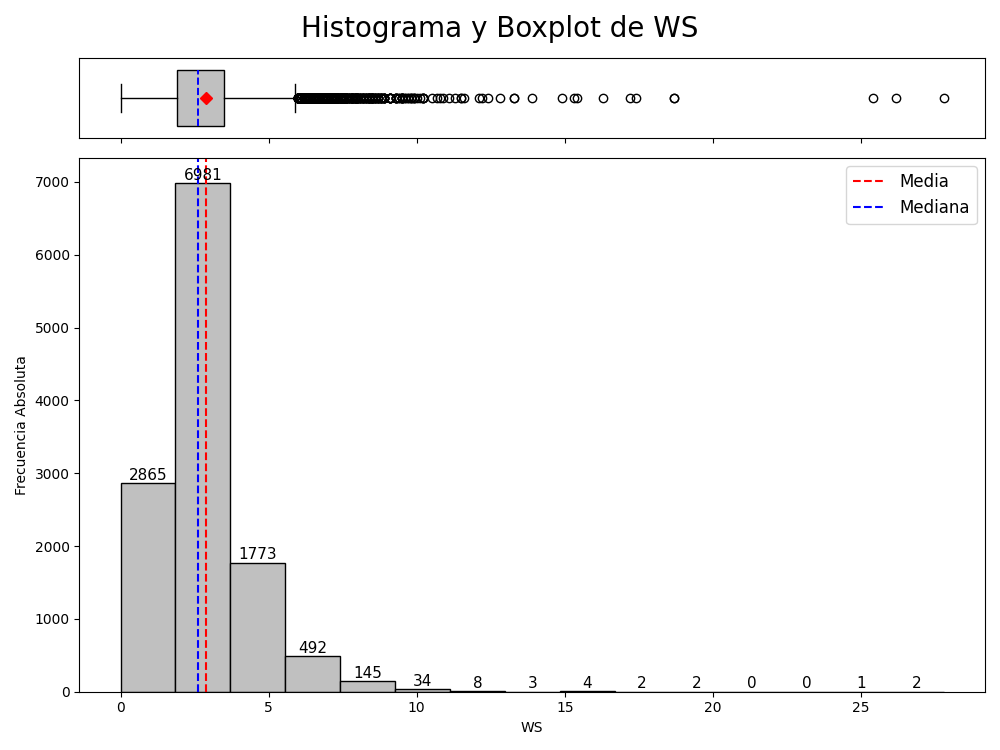
\includegraphics[width=0.4\textwidth]{resultados/global/univariado/WS_histograma.png}
    \label{fig:WS_histograma}
\end{figure}

La velocidad del viento presenta una distribución marcadamente asimétrica a la derecha, con la mayoría de los datos concentrados entre 0 y \SI{5}{\meter\per\second}. Se identifican múltiples valores atípicos altos, correspondientes a eventos aislados de vientos intensos.

\newpage



\subsubsection{Evapotranspiración Potencial (PET)}

\begin{figure}[H]
    \centering
    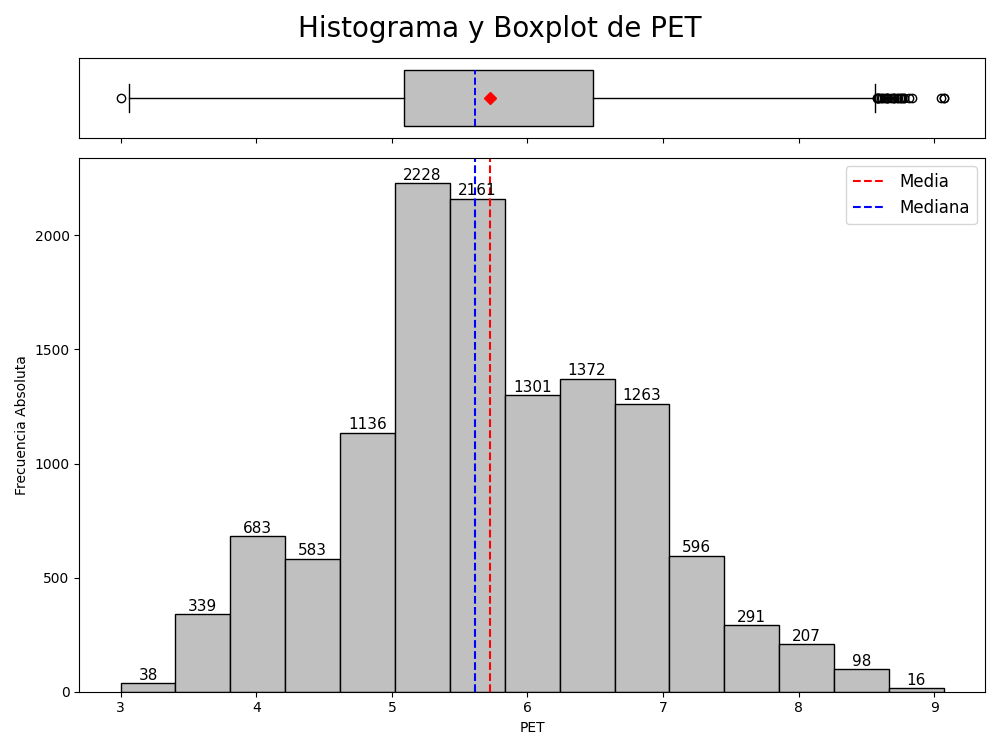
\includegraphics[width=0.4\textwidth]{resultados/global/univariado/PET_histograma.png}
    \caption{Histograma de la Evapotranspiración Potencial (PET).}
    \label{fig:PET_histograma}
\end{figure}

La evapotranspiración potencial muestra una distribución casi simétrica con ligera Skewnessa la derecha. Tanto la Media como la Mediana se ubican en torno a \SI{5.7}{\milli\meter}. Se presentan pocos valores atípicos superiores, lo que indica una distribución bastante estable y consistente.

\section{Análisis Bivariado Global}

A continuación, se presenta el análisis bivariado entre las principales variables climáticas: Precipitación (P), Temperatura (T), Humedad Relativa (RH), Velocidad del Viento (WS) y Evapotranspiración Potencial (PET), utilizando correlaciones lineales, información mutua y gráficos de dispersión.

\subsection{Matriz de Correlación}

\begin{figure}[H]
    \centering
    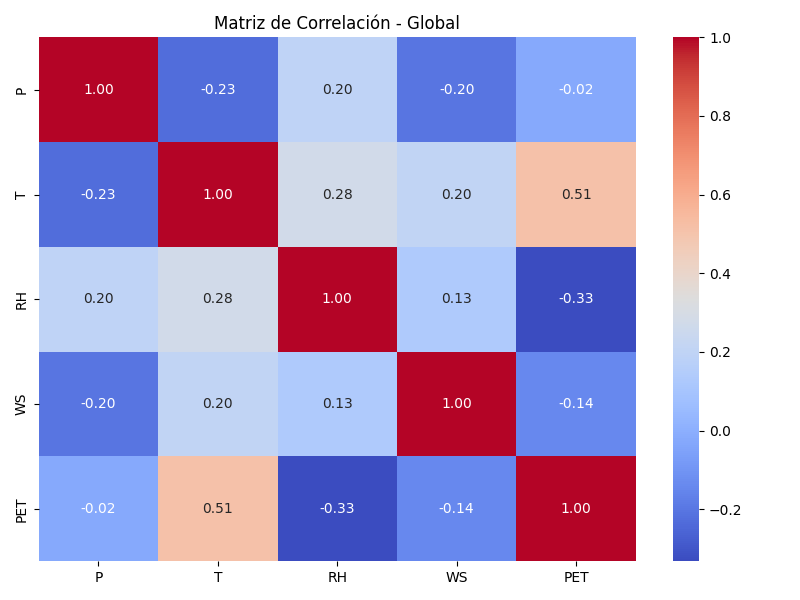
\includegraphics[width=0.7\textwidth]{resultados/global/bivariado/matriz_correlacion.png}
    \caption{Matriz de correlación de variables climáticas globales.}
    \label{fig:matriz_correlacion}
\end{figure}


\subsection{Análisis de Información Mutua}

Las siguientes figuras muestran la información mutua de cada variable considerada como variable dependiente. Esta métrica permite detectar relaciones no necesariamente lineales entre las variables.

\begin{figure}[H]
    \centering
    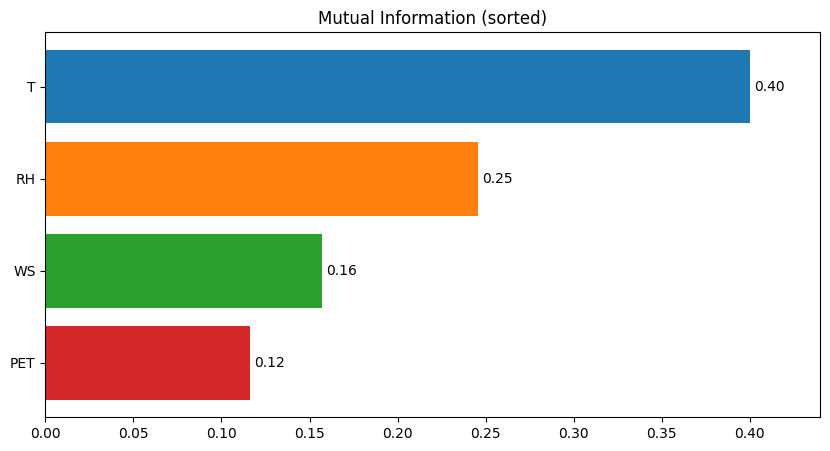
\includegraphics[width=0.4\textwidth]{resultados/global/bivariado/mutual_info_P.png}
    \caption{Información mutua con variable objetivo: Precipitación (P).}
    \label{fig:mutual_info_P}
\end{figure}

\begin{figure}[H]
    \centering
    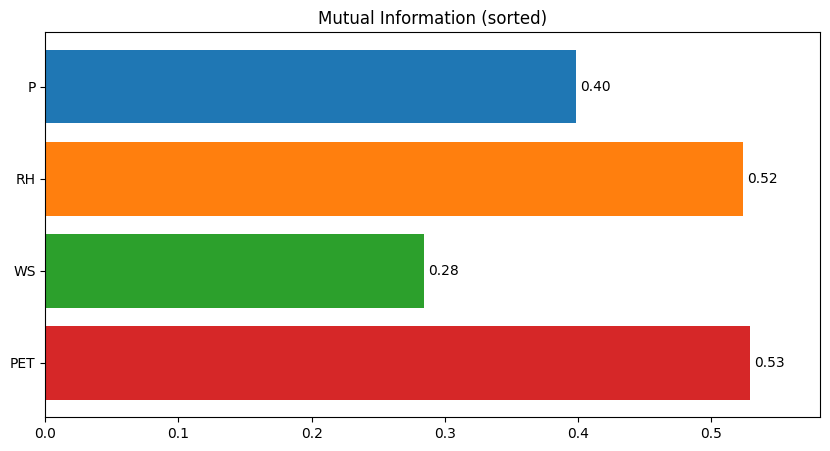
\includegraphics[width=0.4\textwidth]{resultados/global/bivariado/mutual_info_T.png}
    \caption{Información mutua con variable objetivo: Temperatura (T).}
    \label{fig:mutual_info_T}
\end{figure}

\begin{figure}[H]
    \centering
    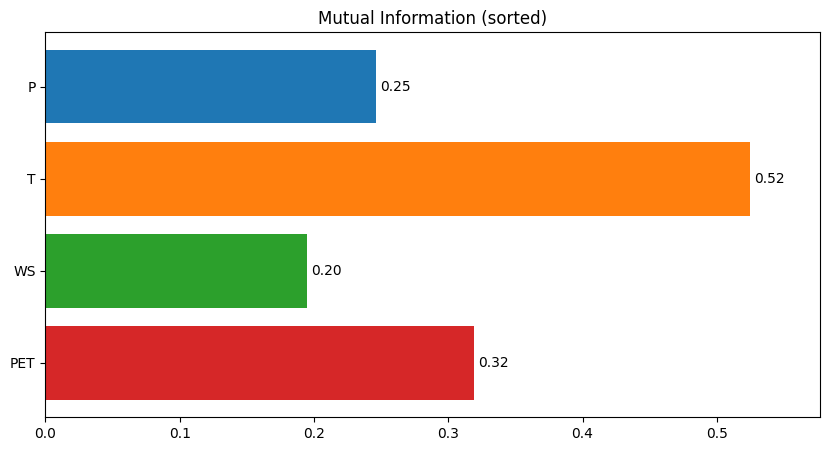
\includegraphics[width=0.4\textwidth]{resultados/global/bivariado/mutual_info_RH.png}
    \caption{Información mutua con variable objetivo: Humedad Relativa (RH).}
    \label{fig:mutual_info_RH}
\end{figure}

\begin{figure}[H]
    \centering
    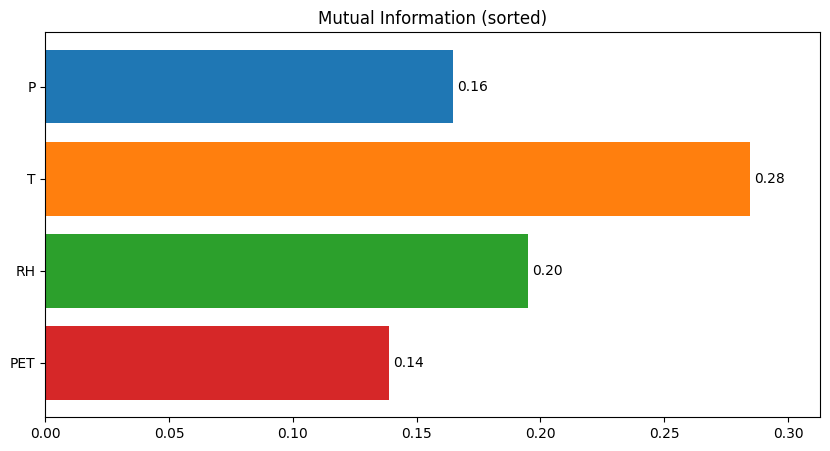
\includegraphics[width=0.4\textwidth]{resultados/global/bivariado/mutual_info_WS.png}
    \caption{Información mutua con variable objetivo: Velocidad del Viento (WS).}
    \label{fig:mutual_info_WS}
\end{figure}

\begin{figure}[H]
    \centering
    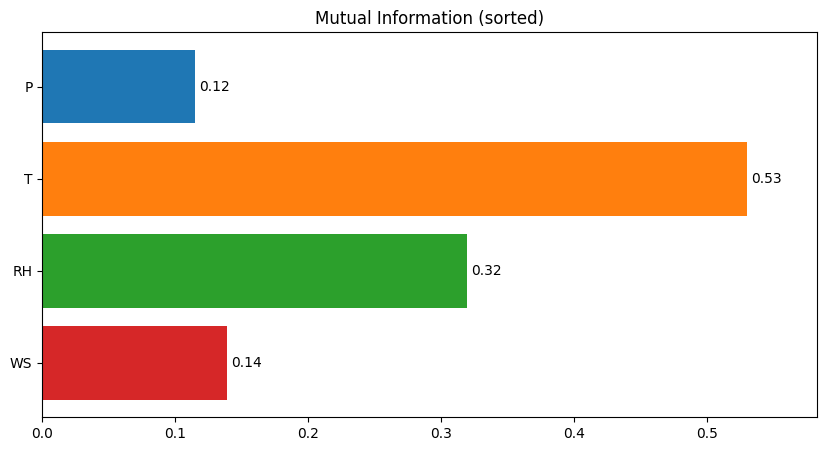
\includegraphics[width=0.4\textwidth]{resultados/global/bivariado/mutual_info_PET.png}
    \caption{Información mutua con variable objetivo: Evapotranspiración Potencial (PET).}
    \label{fig:mutual_info_PET}
\end{figure}

A partir de las Figuras~\ref{fig:mutual_info_P} a~\ref{fig:mutual_info_PET}, se evidencia que la temperatura (T) es consistentemente una de las variables más informativas, especialmente para la predicción de PET, con un valor de información mutua superior a 0.5. Asimismo, la humedad relativa (RH) también muestra valores relevantes en distintos contextos, mientras que la velocidad del viento (WS) y la precipitación (P) presentan menor relevancia relativa. Este análisis complementa a la matriz de correlación al identificar dependencias no lineales.

\subsection{Pairplot Global}

\begin{figure}[H]
    \centering
    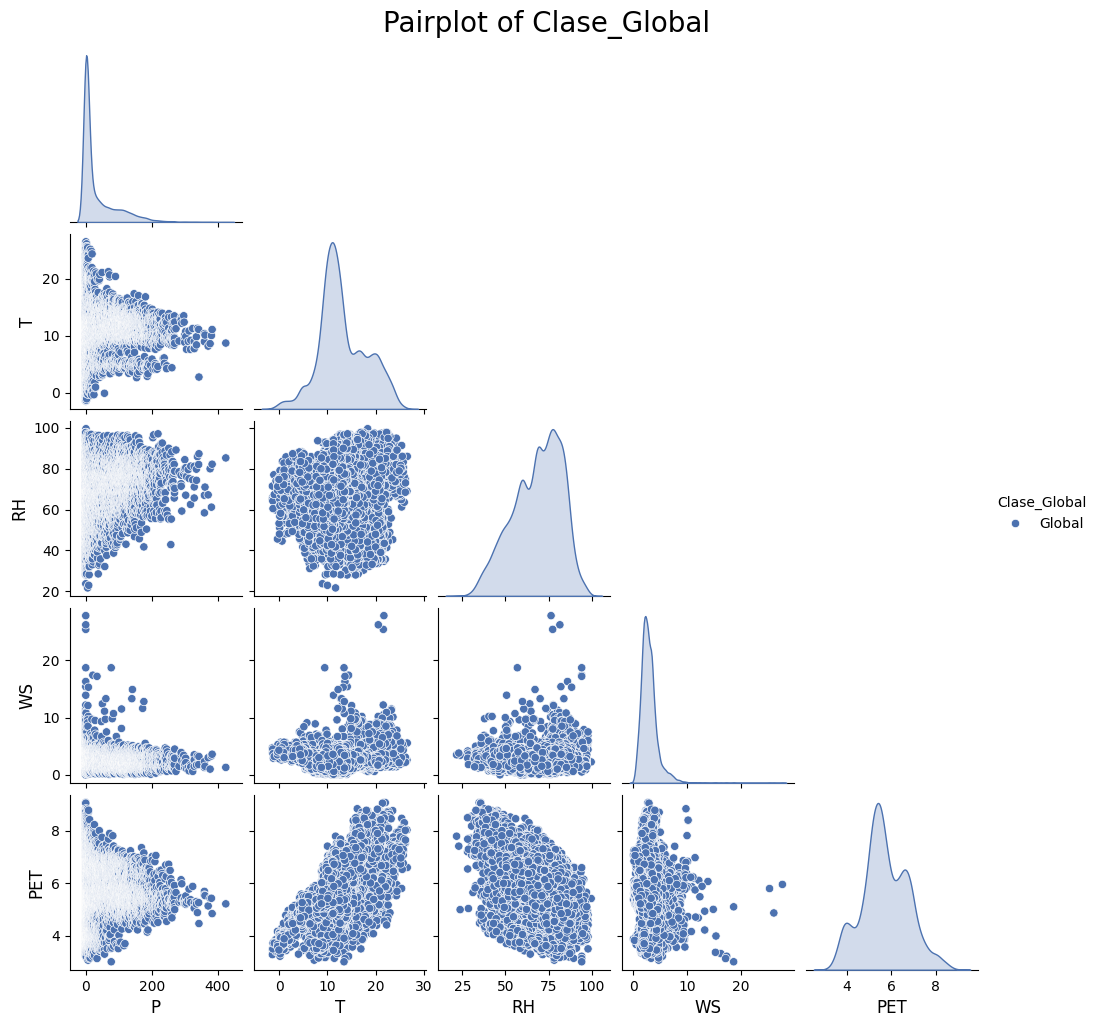
\includegraphics[width=0.4\textwidth]{resultados/global/bivariado/pairplot_global.png}
    \caption{Gráfico de dispersión (pairplot) entre variables climáticas a nivel global.}
    \label{fig:pairplot_global}
\end{figure}

La Figura~\ref{fig:pairplot_global} permite observar visualmente las relaciones bivariadas entre todas las variables. Se destaca una relación creciente entre la temperatura (T) y la evapotranspiración potencial (PET), así como una distribución dispersa entre precipitación (P) y las demás variables, lo que refuerza la débil correlación lineal observada. También se puede observar la distribución de cada variable en la diagonal principal, indicando sesgos o asimetrías en las distribuciones.



\chapter{Analisis de datos por Estación Meteorológica}

\section{Análisis Estadístico de la Estación Ancachuro}

A continuación, se presenta el análisis estadístico descriptivo y exploratorio correspondiente a la estación meteorológica de Ancachuro. Este incluye medidas univariadas por variable y relaciones bivariadas, junto con sus respectivas representaciones gráficas.

\subsection{Estadísticas Descriptivas}

\begin{table}[H]
\centering
\caption{Descriptive statistics of meteorological variables at the Ancachuro station}
\label{tab:stat_ancachuro}
\tiny
\begin{tabular}{lrrrrr}
\toprule
\textbf{Statistic} & \textbf{P (mm)} & \textbf{RH (\%)} & \textbf{T (\textdegree C)} & \textbf{WS (m/s)} & \textbf{PET (mm)} \\
\midrule
$n$         & 648.00  & 648.00  & 648.00  & 648.00  & 648.00 \\
Minimum                 & 0.00    & 49.42   & 6.91    & 0.50    & 3.13   \\
1st Quartile            & 6.30    & 67.27   & 10.41   & 2.20    & 4.95   \\
Median                  & 43.15   & 72.27   & 11.87   & 3.00    & 5.35   \\
Mean                    & 65.60   & 72.45   & 11.58   & 2.96    & 5.26   \\
3rd Quartile            & 113.23  & 77.23   & 12.68   & 3.60    & 5.76   \\
Maximum                 & 296.70  & 93.03   & 14.74   & 5.50    & 6.86   \\
Range                   & 296.70  & 43.61   & 7.83    & 4.70    & 3.73   \\
Interquartile Range     & 106.93  & 9.96    & 2.27    & 1.40    & 0.51   \\
Variance                & 4478.19 & 56.82   & 2.02    & 0.53    & 0.56   \\
Standard Deviation      & 66.92   & 7.54    & 1.42    & 0.51    & 0.51   \\
Coefficient of Variation& 1.02    & 0.10    & 0.12    & 0.31    & 0.15   \\
Skewness              & 0.52    & 0.08    & -0.42   & -0.09   & -0.56  \\
Kurtosis                & 0.01    & -0.20   & -0.57   & -0.56   & -0.25  \\
\bottomrule
\end{tabular}
\end{table}

\textbf{Interpretación:} La precipitación (P) muestra alta variabilidad y Skewnesspositiva, lo que evidencia eventos extremos de lluvia. La humedad relativa (RH) se encuentra centrada entre 67\% y 77\% con baja asimetría. La temperatura (T) presenta simetría leve hacia la izquierda. La velocidad del viento (WS) es relativamente simétrica, mientras que la evapotranspiración potencial (PET) es estable y con Skewnessnegativa.

\subsection{Análisis Univariado}

\subsubsection*{Precipitación (P)}
\begin{figure}[H]
\centering
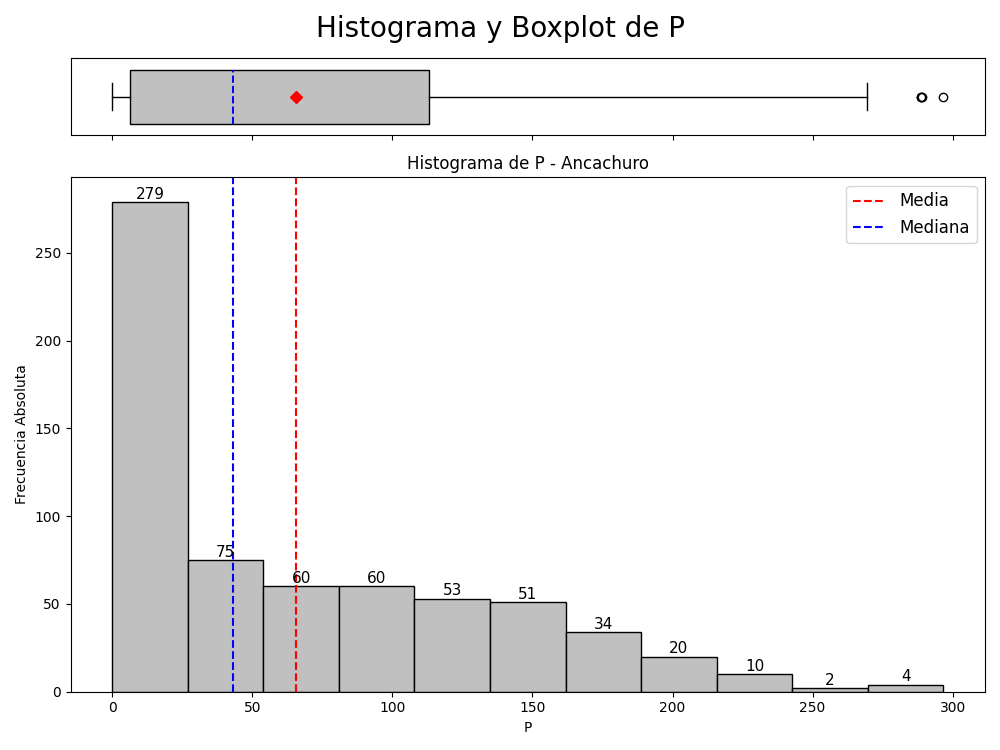
\includegraphics[width=0.4\textwidth]{resultados/por_estacion_meteorologica/Ancachuro/P_histograma.png}
\caption{Histograma de la precipitación (P) en la estación Ancachuro.}
\label{fig:ancachuro_P}
\end{figure}
\textbf{Interpretación:} Se observa una distribución fuertemente sesgada a la derecha. La mayoría de los valores se sitúan por debajo de los 100 mm, aunque existen eventos extremos superiores a 250 mm, lo que explica la diferencia entre la Mean y la mediana.

\subsubsection*{Temperatura (T)}
\begin{figure}[H]
\centering
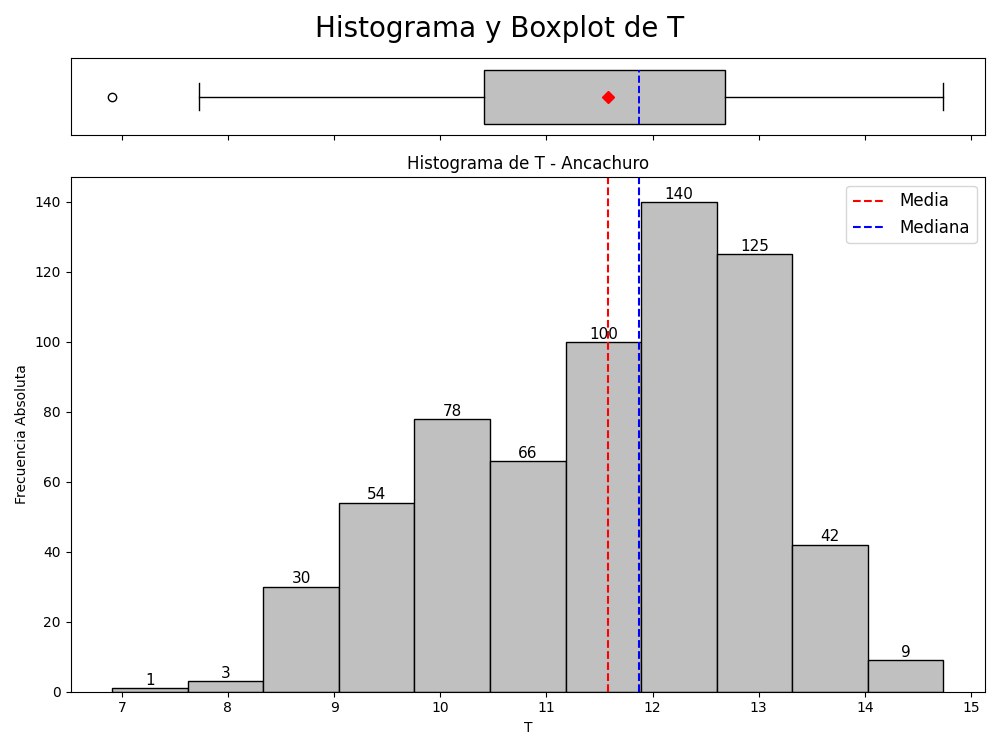
\includegraphics[width=0.4\textwidth]{resultados/por_estacion_meteorologica/Ancachuro/T_histograma.png}
\caption{Histograma de la temperatura (T) en la estación Ancachuro.}
\label{fig:ancachuro_T}
\end{figure}
\textbf{Interpretación:} Distribución relativamente simétrica con ligera Skewnessnegativa. La mayor parte de los valores se concentran entre 10 y 13 \textdegree C.

\subsubsection*{Humedad Relativa (RH)}
\begin{figure}[H]
\centering
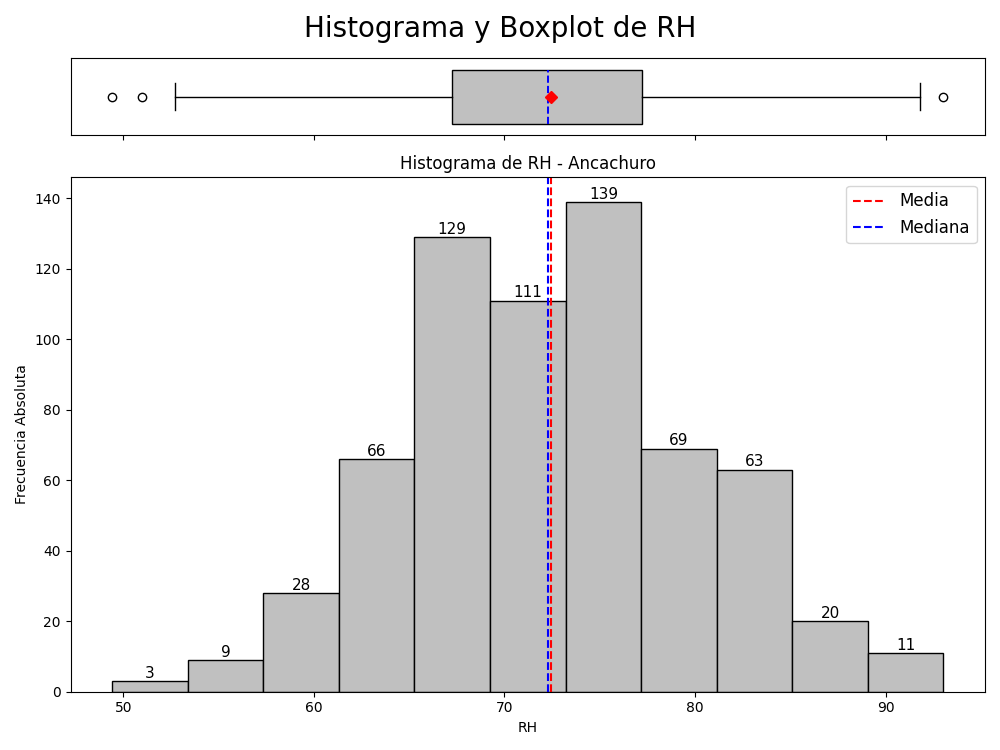
\includegraphics[width=0.4\textwidth]{resultados/por_estacion_meteorologica/Ancachuro/RH_histograma.png}
\caption{Histograma de la humedad relativa (RH) en la estación Ancachuro.}
\label{fig:ancachuro_RH}
\end{figure}
\textbf{Interpretación:} La humedad relativa está centrada entre 65\% y 80\%, con algunos valores extremos bajos y una leve simetría.

\subsubsection*{Velocidad del Viento (WS)}
\begin{figure}[H]
\centering
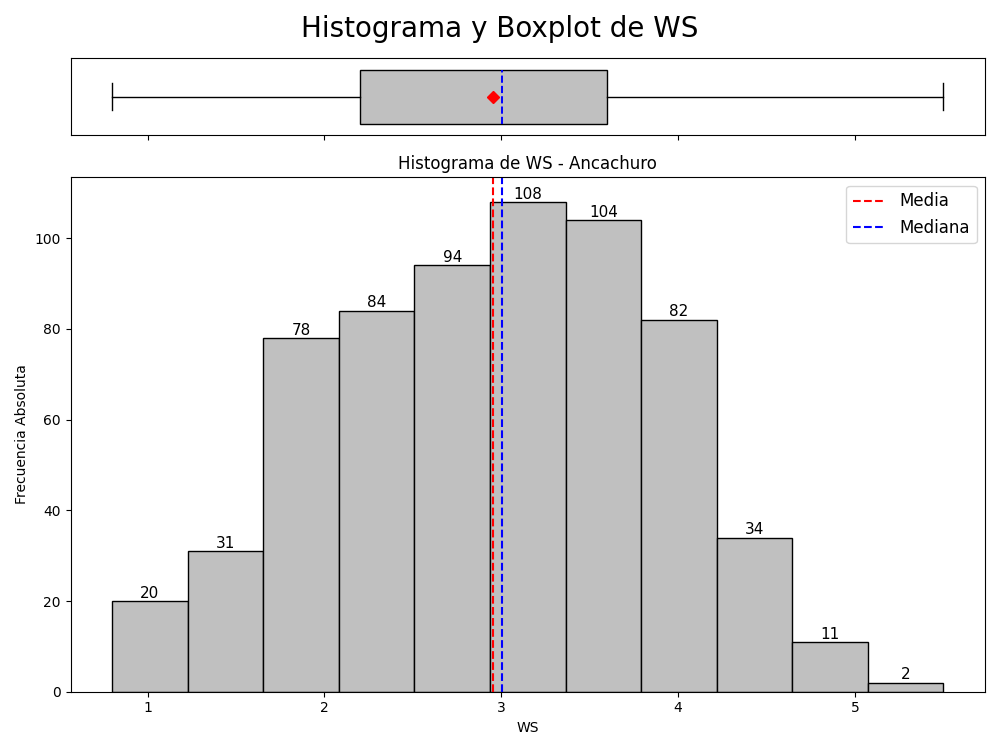
\includegraphics[width=0.4\textwidth]{resultados/por_estacion_meteorologica/Ancachuro/WS_histograma.png}
\caption{Histograma de la velocidad del viento (WS) en la estación Ancachuro.}
\label{fig:ancachuro_WS}
\end{figure}
\textbf{Interpretación:} Distribución simétrica con picos en torno a 3 m/s. La mayoría de los registros se encuentran entre 2 y 4 m/s.

\subsubsection*{Evapotranspiración Potencial (PET)}
\begin{figure}[H]
\centering
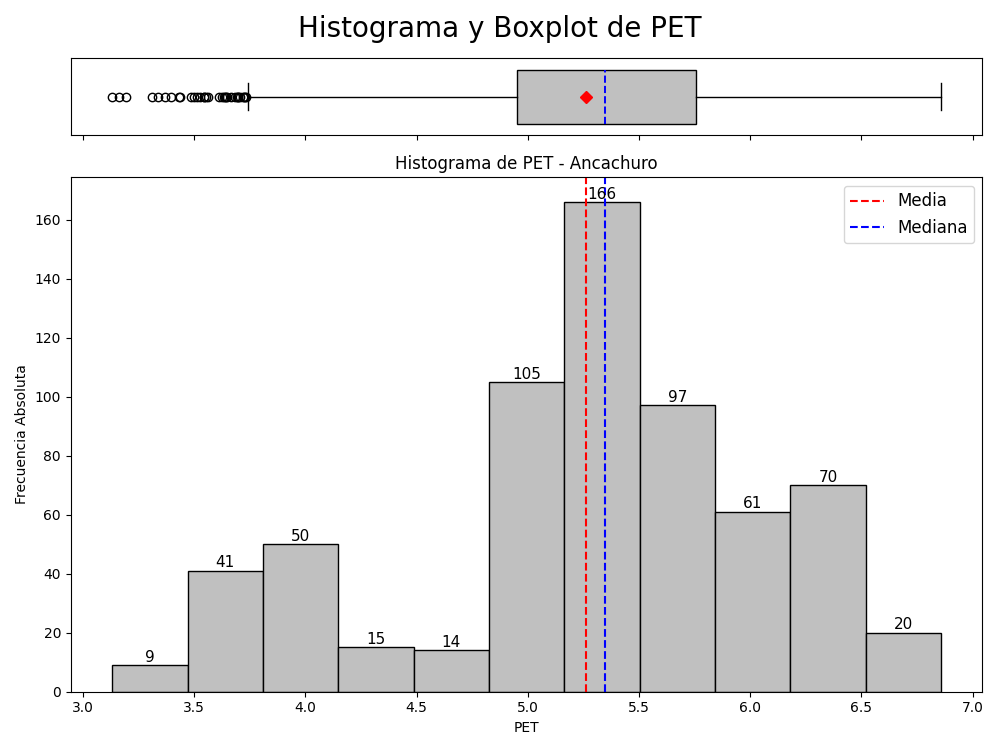
\includegraphics[width=0.4\textwidth]{resultados/por_estacion_meteorologica/Ancachuro/PET_histograma.png}
\caption{Histograma de la evapotranspiración potencial (PET) en la estación Ancachuro.}
\label{fig:ancachuro_PET}
\end{figure}
\textbf{Interpretación:} Distribución bastante concentrada con leve Skewnessnegativa. Valores centrados en torno a 5.2 mm con escasos valores extremos.

\subsection{Análisis Bivariado}

\subsubsection*{Matriz de Correlación}
\begin{figure}[H]
\centering
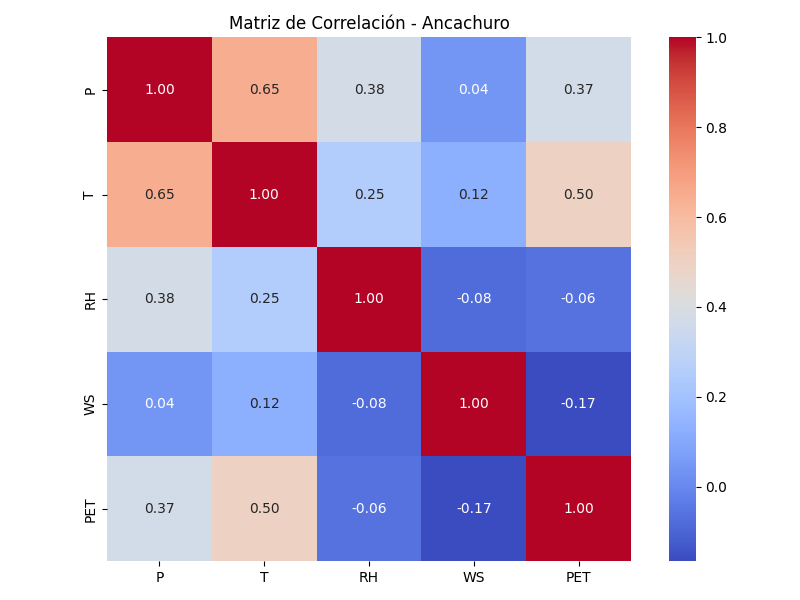
\includegraphics[width=0.45\textwidth]{resultados/por_estacion_meteorologica/Ancachuro/matriz_correlacion.png}
\caption{Matriz de correlación de las variables meteorológicas en Ancachuro.}
\label{fig:ancachuro_corr}
\end{figure}
\textbf{Interpretación:} Se observa correlación positiva entre temperatura (T) y PET ($r \approx 0.50$), y entre precipitación (P) y temperatura (T) ($r \approx 0.45$).

\subsubsection*{Gráfico de Pares (Pairplot)}
\begin{figure}[H]
\centering
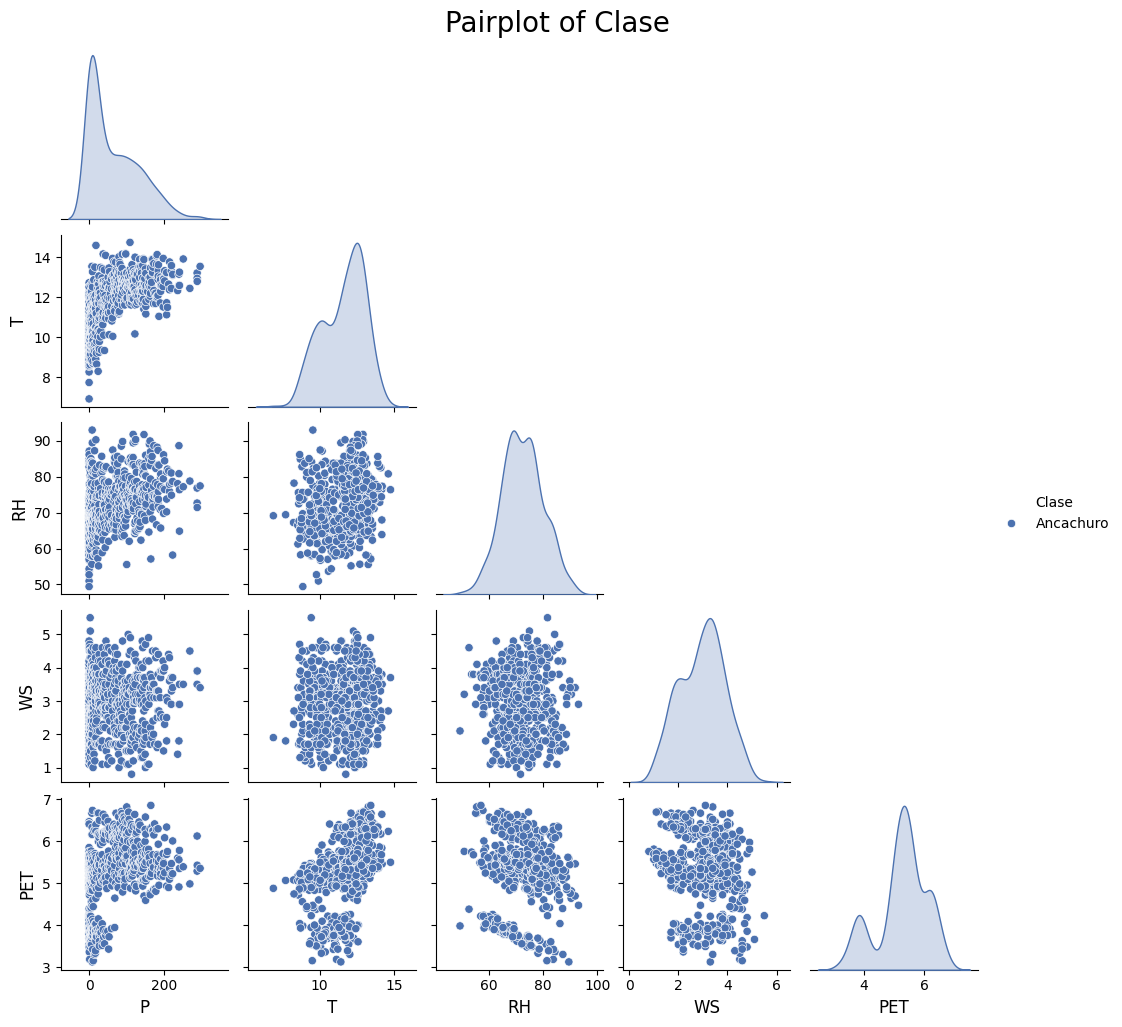
\includegraphics[width=0.45\textwidth]{resultados/por_estacion_meteorologica/Ancachuro/pairplot.png}
\caption{Pairplot de las variables meteorológicas en la estación Ancachuro.}
\label{fig:ancachuro_pairplot}
\end{figure}
\textbf{Interpretación:} El pairplot evidencia patrones visuales similares a los encontrados en la matriz de correlación. Se destaca la asociación positiva entre T y PET, y una relación moderada entre P y T. RH y WS presentan distribuciones dispersas respecto a las demás variables.







\section{Análisis Estadístico de la Estación Andahuaylas}

A continuación, se presenta el análisis estadístico descriptivo y exploratorio correspondiente a la estación meteorológica de Andahuaylas. Este incluye medidas univariadas por variable y relaciones bivariadas, junto con sus respectivas representaciones gráficas.

\subsection{Estadísticas Descriptivas}

\begin{table}[H]
\centering
\caption{Descriptive statistics of meteorological variables at the Andahuaylas station}
\label{tab:stat_andahuaylas}
\tiny
\begin{tabular}{lrrrrr}
\toprule
\textbf{Statistic} & \textbf{P (mm)} & \textbf{RH (\%)} & \textbf{T (\textdegree C)} & \textbf{WS (m/s)} & \textbf{PET (mm)} \\
\midrule
$n$         & 648.00  & 648.00  & 648.00  & 648.00  & 648.00 \\
Minimum                 & 0.00    & 58.45   & 10.35   & 0.50    & 3.48   \\
1st Quartile            & 14.23   & 74.08   & 12.37   & 2.00    & 4.53   \\
Median                  & 39.55   & 78.84   & 13.59   & 2.50    & 5.10   \\
Mean                    & 54.57   & 80.18   & 13.42   & 2.49    & 5.03   \\
3rd Quartile            & 88.02   & 86.49   & 14.47   & 2.74    & 5.50   \\
Maximum                 & 251.50  & 97.12   & 16.83   & 6.20    & 6.45   \\
Range                   & 251.50  & 38.67   & 6.48    & 5.30    & 2.97   \\
Interquartile Range     & 73.80   & 12.42   & 2.10    & 0.74    & 0.57   \\
Variance                & 2450.00 & 65.16   & 1.65    & 0.51    & 0.36   \\
Standard Deviation      & 49.50   & 8.07    & 1.29    & 0.78    & 0.50   \\
Coefficient of Variation& 0.51    & 0.10    & 0.10    & 0.31    & 0.12   \\
Skewness              & 1.06    & 0.24    & -0.24   & 1.39    & -0.13  \\
Kurtosis                & 0.54    & -0.76   & -0.75   & 3.48    & -0.57  \\
\bottomrule
\end{tabular}
\end{table}

\textbf{Interpretación:} La precipitación (P) muestra alta variabilidad y Skewnesspositiva, lo que evidencia eventos extremos de lluvia. La humedad relativa (RH) se encuentra centrada entre 74\% y 86\%, con ligera Skewnesspositiva. La temperatura (T) presenta simetría leve hacia la izquierda. La velocidad del viento (WS) es asimétrica con presencia de ráfagas, mientras que la evapotranspiración potencial (PET) es relativamente estable con Skewnessnegativa leve.

\subsection{Análisis Univariado}

\subsubsection*{Precipitación (P)}
\begin{figure}[H]
\centering
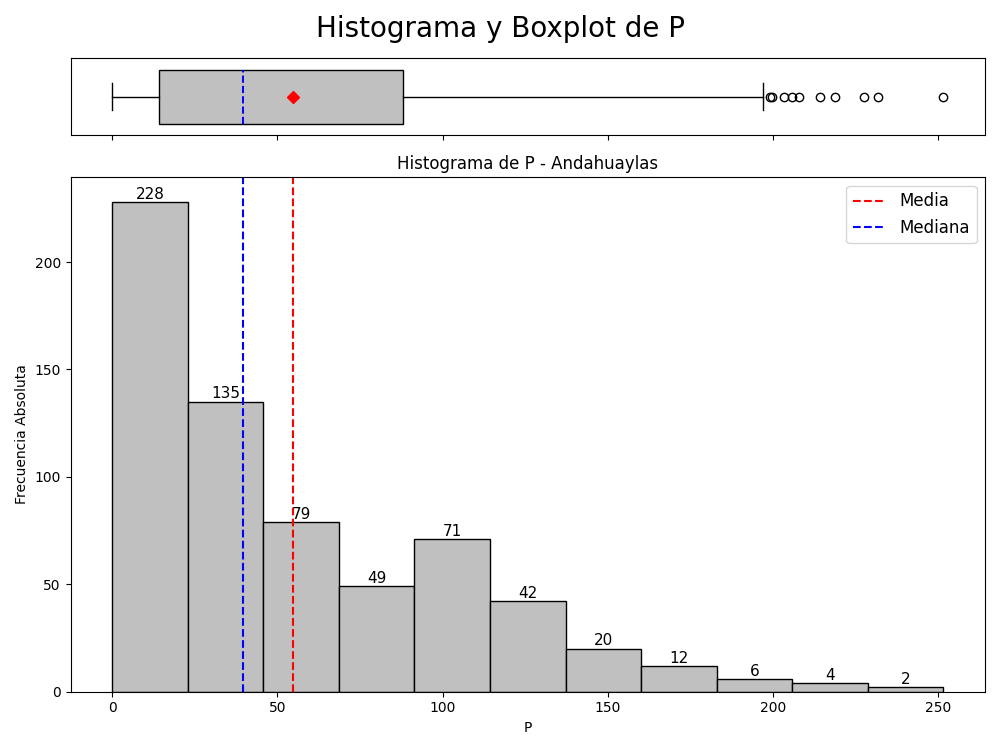
\includegraphics[width=0.4\textwidth]{resultados/por_estacion_meteorologica/Andahuaylas/P_histograma.png}
\caption{Histograma y boxplot de la precipitación (P) en la estación Andahuaylas.}
\label{fig:andahuaylas_P}
\end{figure}
\textbf{Interpretación:} Distribución altamente asimétrica a la derecha. La mayoría de los valores se concentran por debajo de los 100 mm, con presencia de eventos extremos superiores a 250 mm.

\subsubsection*{Temperatura (T)}
\begin{figure}[H]
\centering
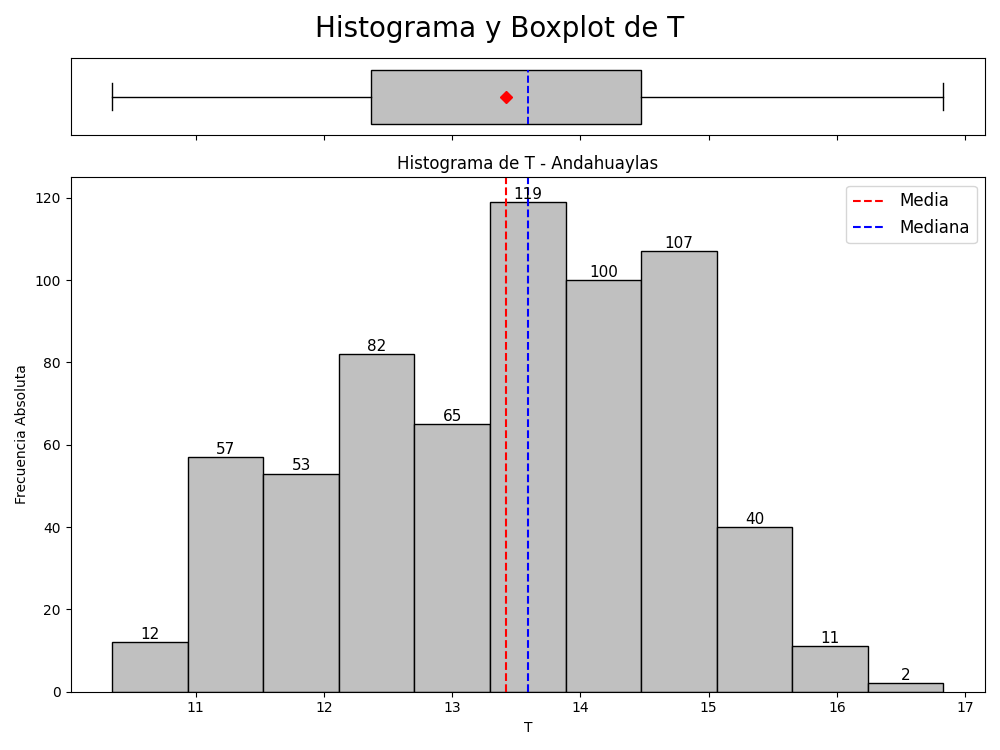
\includegraphics[width=0.4\textwidth]{resultados/por_estacion_meteorologica/Andahuaylas/T_histograma.png}
\caption{Histograma y boxplot de la temperatura (T) en la estación Andahuaylas.}
\label{fig:andahuaylas_T}
\end{figure}
\textbf{Interpretación:} Distribución moderadamente simétrica con leve sesgo negativo. La mayoría de los registros se encuentran entre 12 y 15 \textdegree C.

\subsubsection*{Humedad Relativa (RH)}
\begin{figure}[H]
\centering
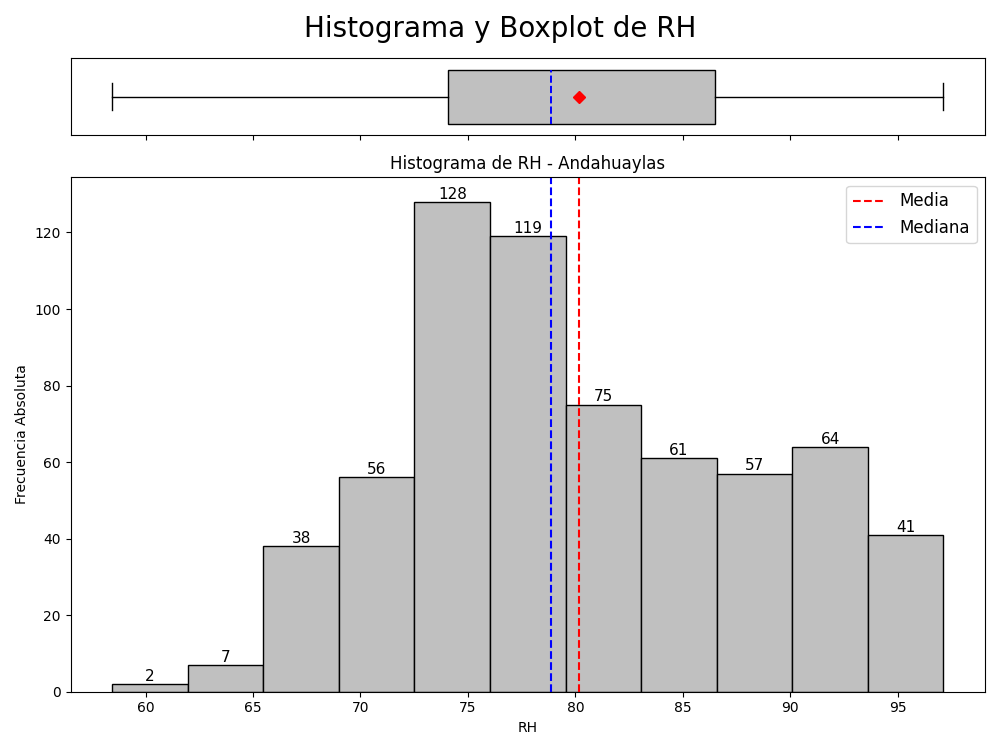
\includegraphics[width=0.4\textwidth]{resultados/por_estacion_meteorologica/Andahuaylas/RH_histograma.png}
\caption{Histograma y boxplot de la humedad relativa (RH) en la estación Andahuaylas.}
\label{fig:andahuaylas_RH}
\end{figure}
\textbf{Interpretación:} La RH está centrada entre 70\% y 90\%, con Skewnesspositiva leve y valores extremos bajos ocasionales.

\subsubsection*{Velocidad del Viento (WS)}
\begin{figure}[H]
\centering
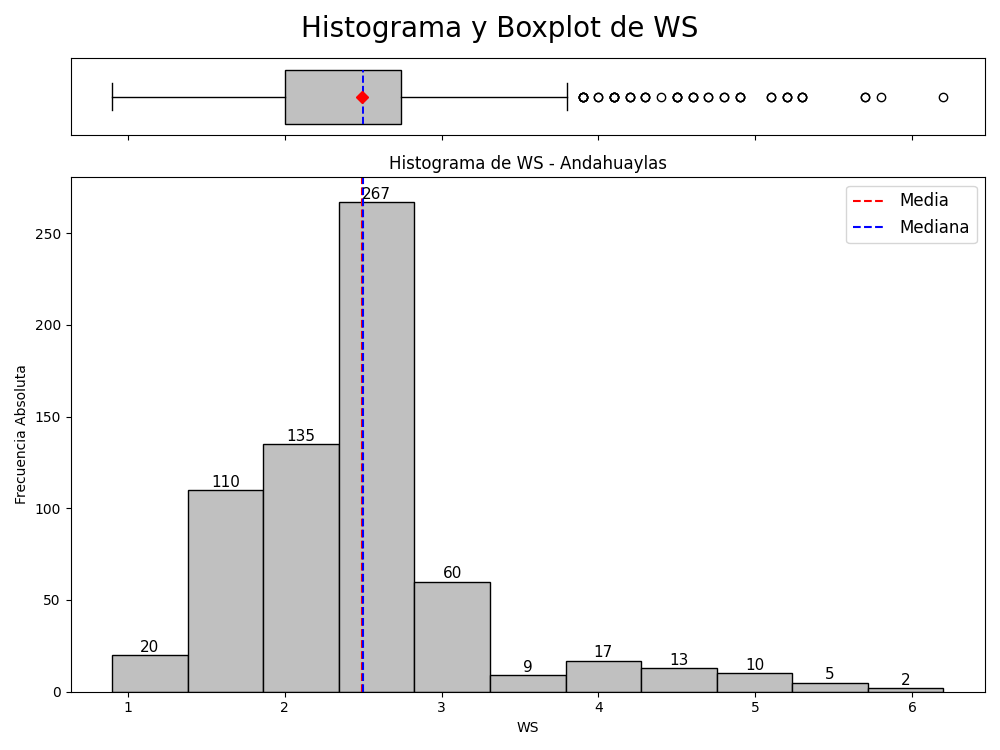
\includegraphics[width=0.4\textwidth]{resultados/por_estacion_meteorologica/Andahuaylas/WS_histograma.png}
\caption{Histograma y boxplot de la velocidad del viento (WS) en la estación Andahuaylas.}
\label{fig:andahuaylas_WS}
\end{figure}
\textbf{Interpretación:} Distribución sesgada con concentración en valores bajos (2 a 3 m/s), pero con outliers que representan ráfagas inusuales de hasta 6.2 m/s.

\subsubsection*{Evapotranspiración Potencial (PET)}
\begin{figure}[H]
\centering
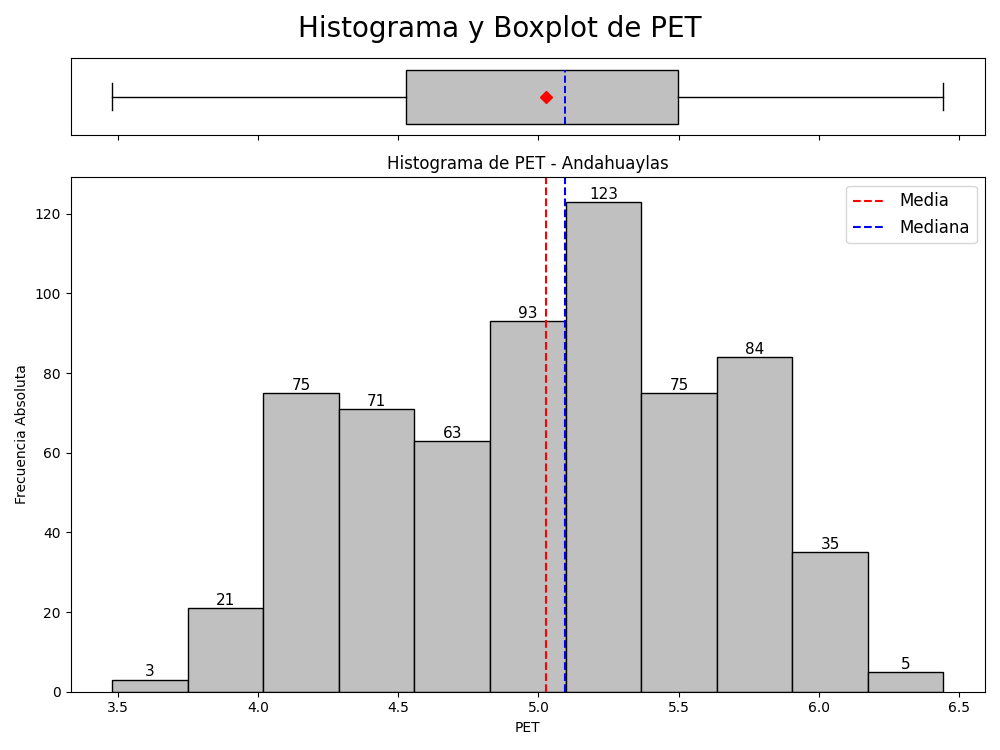
\includegraphics[width=0.4\textwidth]{resultados/por_estacion_meteorologica/Andahuaylas/PET_histograma.png}
\caption{Histograma y boxplot de la evapotranspiración potencial (PET) en la estación Andahuaylas.}
\label{fig:andahuaylas_PET}
\end{figure}
\textbf{Interpretación:} Distribución relativamente estable, con valores entre 4.5 y 6.5 mm y ligera Skewnessnegativa.

\subsection{Análisis Bivariado}

\subsubsection*{Matriz de Correlación}
\begin{figure}[H]
\centering
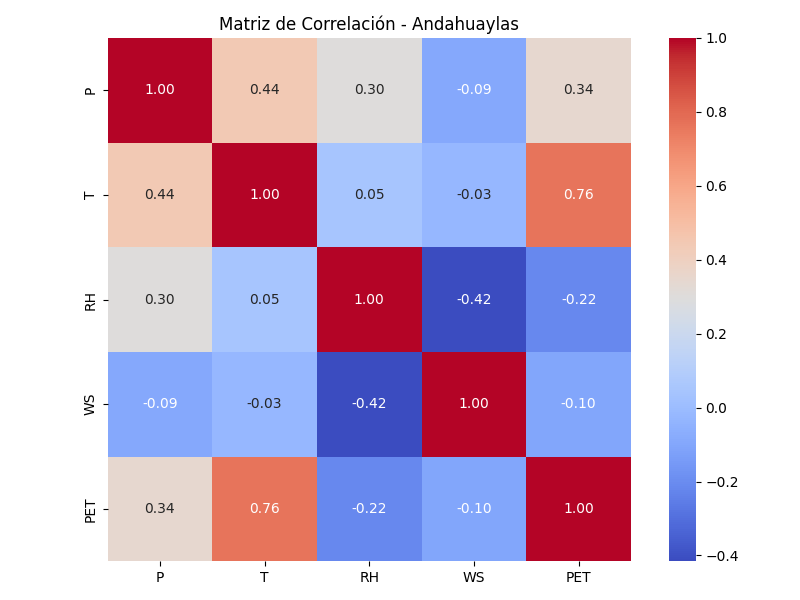
\includegraphics[width=0.4\textwidth]{resultados/por_estacion_meteorologica/Andahuaylas/matriz_correlacion.png}
\caption{Matriz de correlación de las variables meteorológicas en Andahuaylas.}
\label{fig:andahuaylas_corr}
\end{figure}
\textbf{Interpretación:} Se evidencia fuerte correlación positiva entre temperatura (T) y evapotranspiración potencial (PET) (\(r = 0.76\)). También se observa correlación moderada entre P y T (\(r = 0.44\)). Las correlaciones entre RH, WS y otras variables son generalmente bajas o negativas.

\subsubsection*{Gráfico de Pares (Pairplot)}
\begin{figure}[H]
\centering
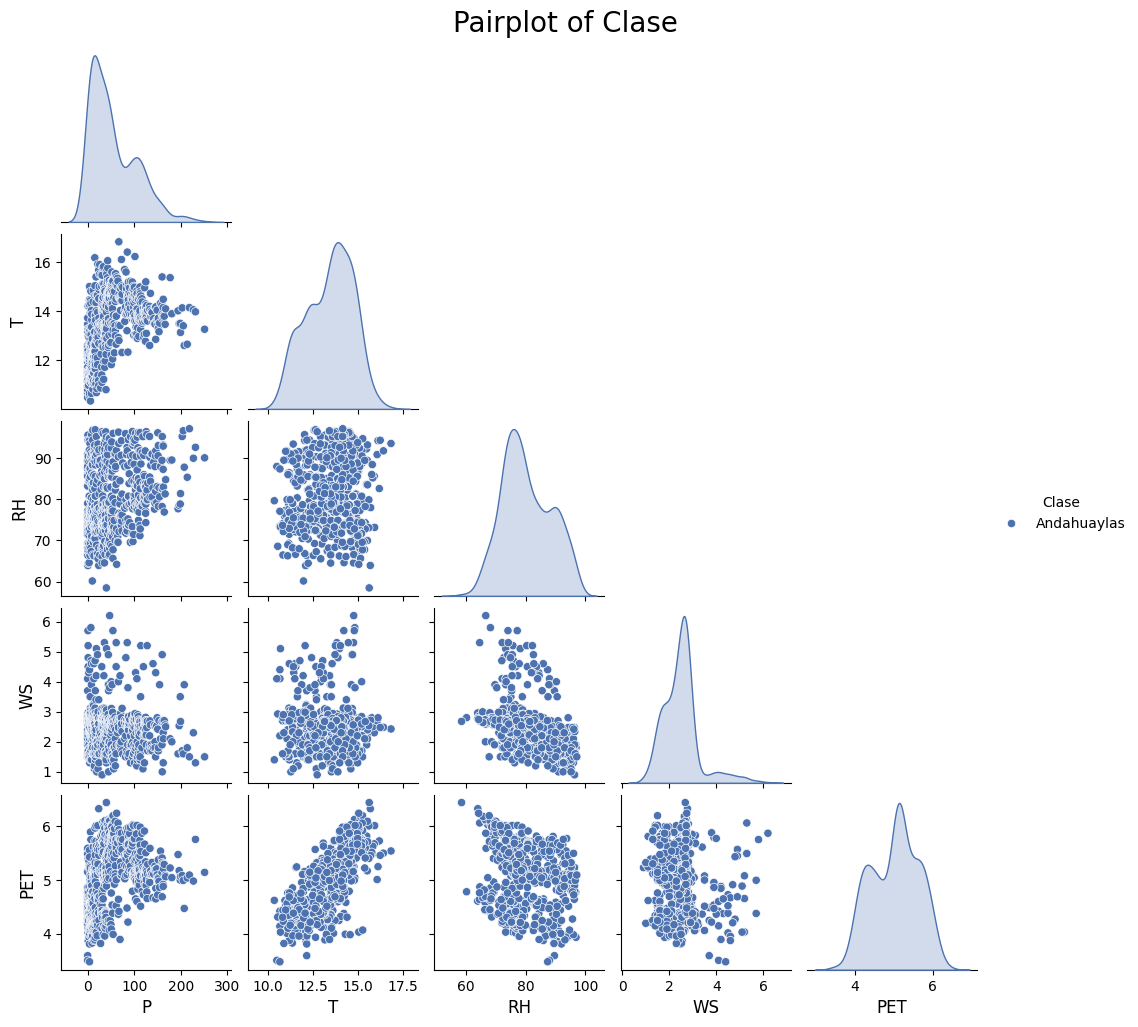
\includegraphics[width=0.45\textwidth]{resultados/por_estacion_meteorologica/Andahuaylas/pairplot.png}
\caption{Pairplot de las variables meteorológicas en la estación Andahuaylas.}
\label{fig:andahuaylas_pairplot}
\end{figure}
\textbf{Interpretación:} El gráfico de dispersión confirma la fuerte asociación entre T y PET, y una relación moderada entre P y T. RH presenta relación inversa con PET y WS. Las combinaciones con WS tienden a ser más dispersas.






\section{Análisis Estadístico de la Estación Ancachuro}

A continuación, se presenta el análisis estadístico descriptivo y exploratorio correspondiente a la estación meteorológica de Ancachuro. Este incluye medidas univariadas por variable y relaciones bivariadas, junto con sus respectivas representaciones gráficas.

\subsection{Estadísticas Descriptivas}

\begin{table}[H]
\centering
\caption{Descriptive statistics of meteorological variables at the Ancachuro station}
\label{tab:stat_ancachuro}
\tiny
\begin{tabular}{lrrrrr}
\toprule
\textbf{Statistic} & \textbf{P (mm)} & \textbf{RH (\%)} & \textbf{T (\textdegree C)} & \textbf{WS (m/s)} & \textbf{PET (mm)} \\
\midrule
$n$          & 648.00  & 648.00  & 648.00  & 648.00  & 648.00 \\
Minimum                 & 0.00    & 49.42   & 6.91    & 0.50    & 3.13   \\
1st Quartile            & 6.30    & 67.27   & 10.41   & 2.20    & 4.95   \\
Median                  & 43.15   & 72.27   & 11.87   & 3.00    & 5.35   \\
Mean                    & 65.60   & 72.45   & 11.58   & 2.96    & 5.26   \\
3rd Quartile            & 113.23  & 77.23   & 12.68   & 3.60    & 5.76   \\
Maximum                 & 296.70  & 93.03   & 14.74   & 5.50    & 6.86   \\
Range                   & 296.70  & 43.61   & 7.83    & 4.70    & 3.73   \\
Interquartile Range     & 106.93  & 9.96    & 2.27    & 1.40    & 0.51   \\
Variance                & 4478.19 & 56.82   & 2.02    & 0.53    & 0.56   \\
Standard Deviation      & 66.92   & 7.54    & 1.42    & 0.51    & 0.51   \\
Coefficient of Variation& 1.02    & 0.10    & 0.12    & 0.31    & 0.15   \\
Skewness              & 0.52    & 0.08    & -0.42   & -0.09   & -0.56  \\
Kurtosis                & 0.01    & -0.20   & -0.57   & -0.56   & -0.25  \\
\bottomrule
\end{tabular}
\end{table}

\textbf{Interpretación:} La precipitación (P) muestra alta variabilidad y Skewnesspositiva, lo que evidencia eventos extremos de lluvia. La humedad relativa (RH) se encuentra centrada entre 67\% y 77\% con baja asimetría. La temperatura (T) presenta simetría leve hacia la izquierda. La velocidad del viento (WS) es relativamente simétrica, mientras que la evapotranspiración potencial (PET) es estable y con Skewnessnegativa.

\subsection{Análisis Univariado}

\subsubsection*{Precipitación (P)}
\begin{figure}[H]
\centering
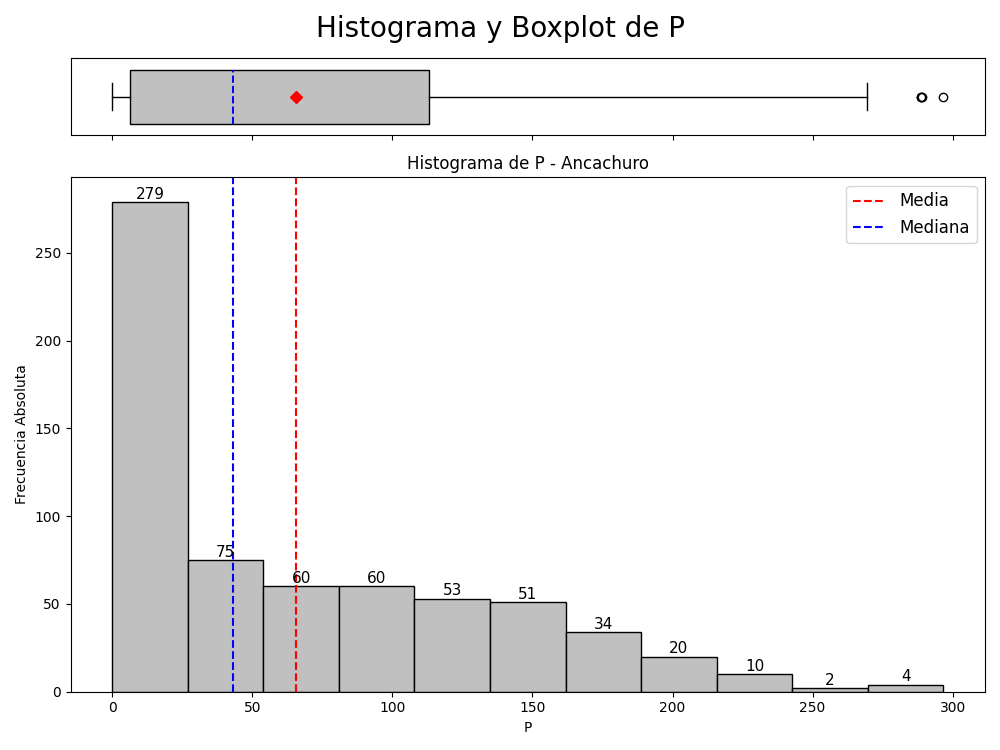
\includegraphics[width=0.4\textwidth]{resultados/por_estacion_meteorologica/Ancachuro/P_histograma.png}
\caption{Histograma de la precipitación (P) en la estación Ancachuro.}
\label{fig:ancachuro_P}
\end{figure}
\textbf{Interpretación:} Se observa una distribución fuertemente sesgada a la derecha. La mayoría de los valores se sitúan por debajo de los 100 mm, aunque existen eventos extremos superiores a 250 mm, lo que explica la diferencia entre la Mean y la mediana.

\subsubsection*{Temperatura (T)}
\begin{figure}[H]
\centering
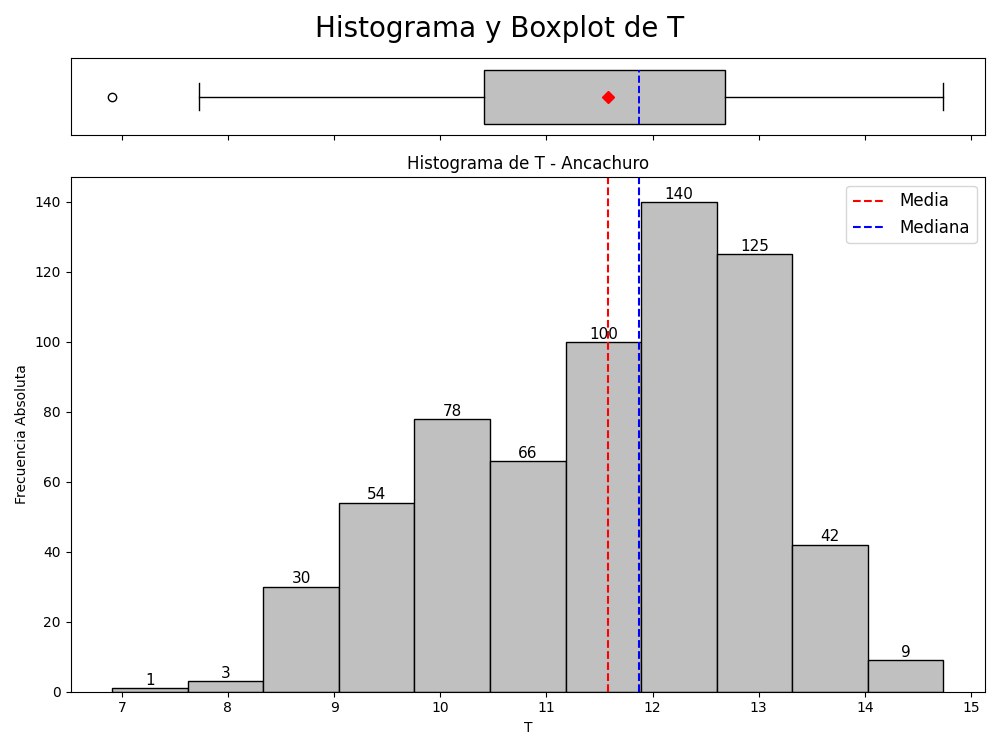
\includegraphics[width=0.4\textwidth]{resultados/por_estacion_meteorologica/Ancachuro/T_histograma.png}
\caption{Histograma de la temperatura (T) en la estación Ancachuro.}
\label{fig:ancachuro_T}
\end{figure}
\textbf{Interpretación:} Distribución relativamente simétrica con ligera Skewnessnegativa. La mayor parte de los valores se concentran entre 10 y 13 \textdegree C.

\subsubsection*{Humedad Relativa (RH)}
\begin{figure}[H]
\centering
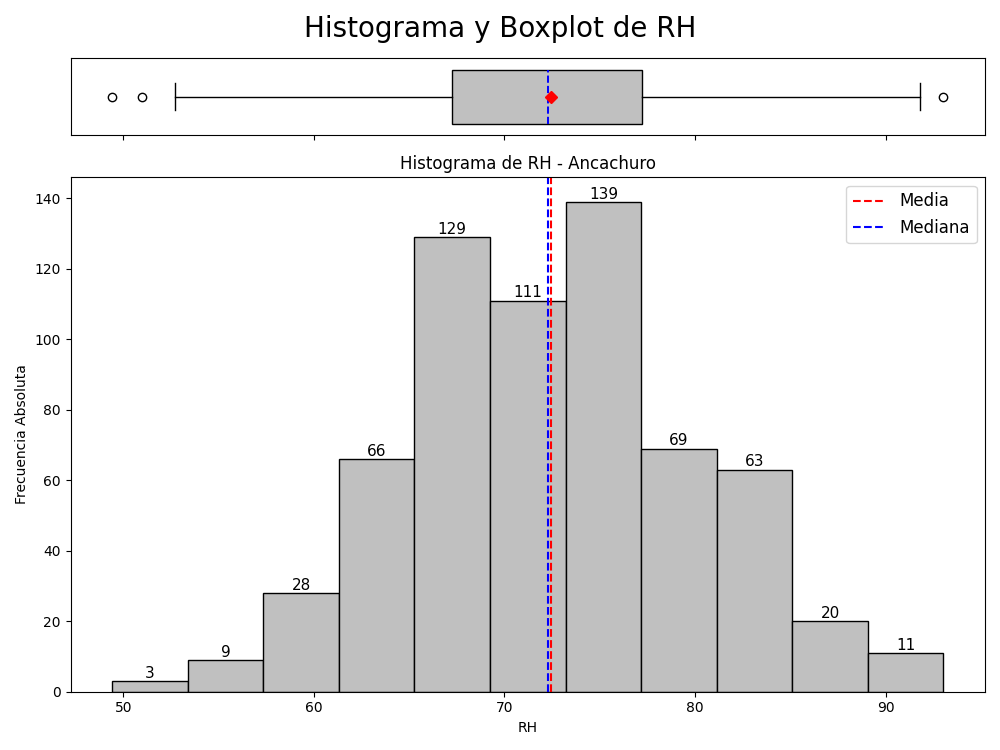
\includegraphics[width=0.4\textwidth]{resultados/por_estacion_meteorologica/Ancachuro/RH_histograma.png}
\caption{Histograma de la humedad relativa (RH) en la estación Ancachuro.}
\label{fig:ancachuro_RH}
\end{figure}
\textbf{Interpretación:} La humedad relativa está centrada entre 65\% y 80\%, con algunos valores extremos bajos y una leve simetría.

\subsubsection*{Velocidad del Viento (WS)}
\begin{figure}[H]
\centering
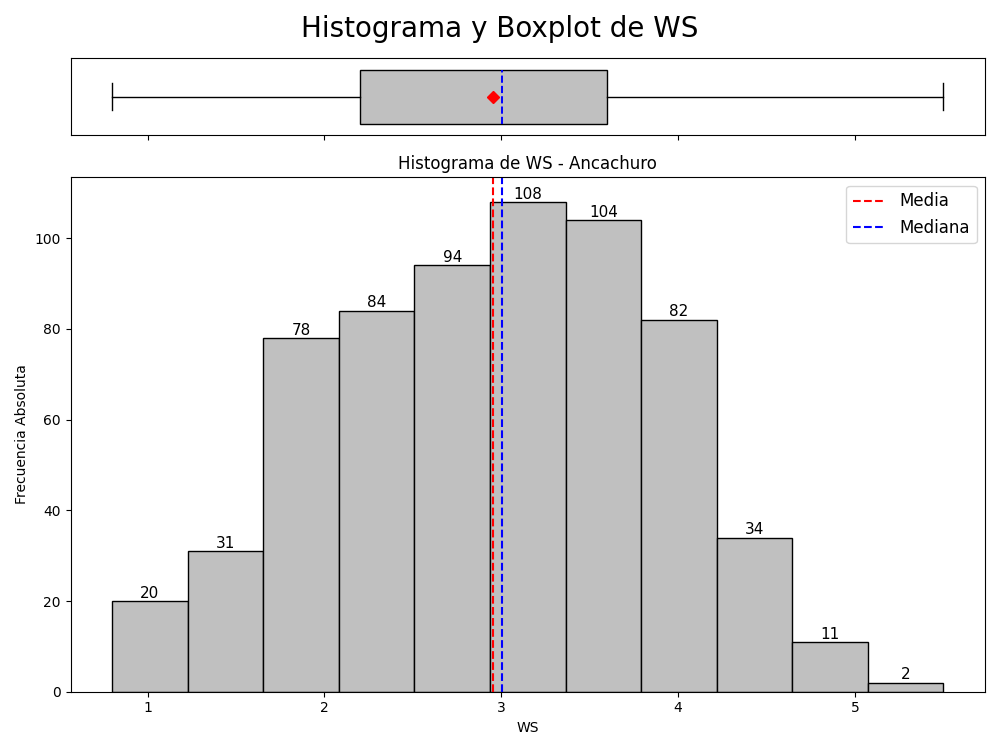
\includegraphics[width=0.4\textwidth]{resultados/por_estacion_meteorologica/Ancachuro/WS_histograma.png}
\caption{Histograma de la velocidad del viento (WS) en la estación Ancachuro.}
\label{fig:ancachuro_WS}
\end{figure}
\textbf{Interpretación:} Distribución simétrica con picos en torno a 3 m/s. La mayoría de los registros se encuentran entre 2 y 4 m/s.

\subsubsection*{Evapotranspiración Potencial (PET)}
\begin{figure}[H]
\centering
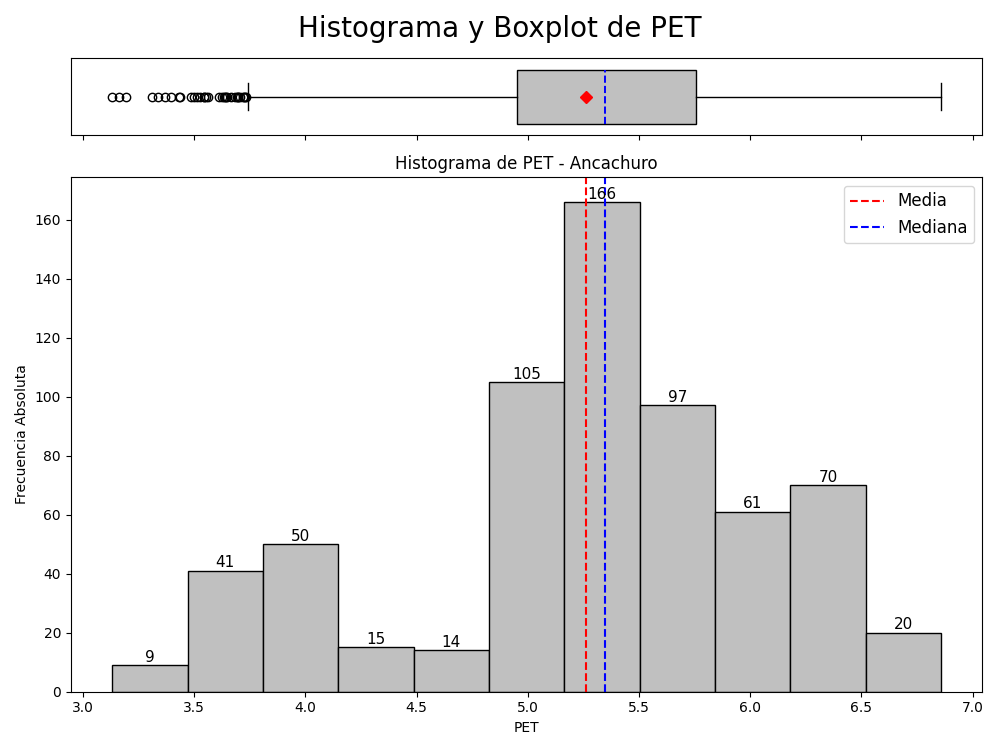
\includegraphics[width=0.4\textwidth]{resultados/por_estacion_meteorologica/Ancachuro/PET_histograma.png}
\caption{Histograma de la evapotranspiración potencial (PET) en la estación Ancachuro.}
\label{fig:ancachuro_PET}
\end{figure}
\textbf{Interpretación:} Distribución bastante concentrada con leve Skewnessnegativa. Valores centrados en torno a 5.2 mm con escasos valores extremos.

\subsection{Análisis Bivariado}

\subsubsection*{Matriz de Correlación}
\begin{figure}[H]
\centering
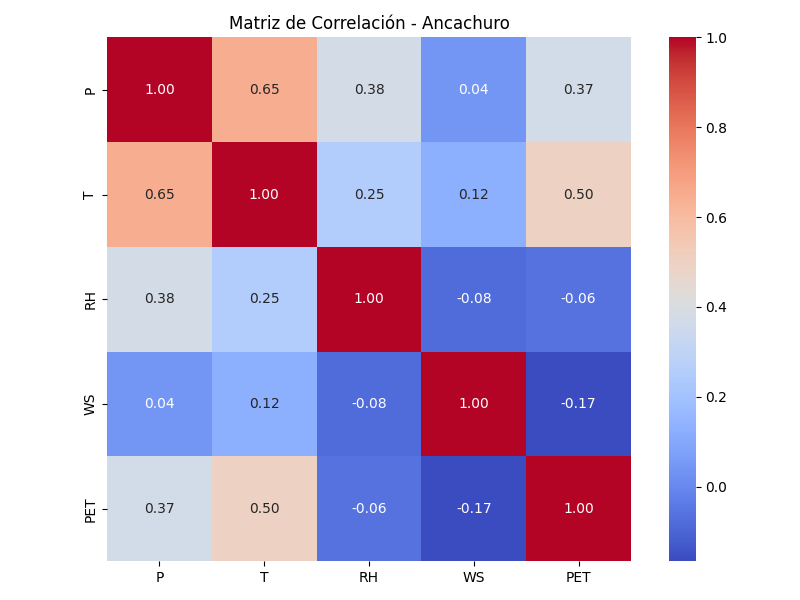
\includegraphics[width=0.45\textwidth]{resultados/por_estacion_meteorologica/Ancachuro/matriz_correlacion.png}
\caption{Matriz de correlación de las variables meteorológicas en Ancachuro.}
\label{fig:ancachuro_corr}
\end{figure}
\textbf{Interpretación:} Se observa correlación positiva entre temperatura (T) y PET (\(r = 0.50\)), y entre precipitación (P) y temperatura (T) (\(r = 0.45\)). La humedad relativa (RH) muestra correlaciones débiles con las demás variables.

\subsubsection*{Gráfico de Pares (Pairplot)}
\begin{figure}[H]
\centering
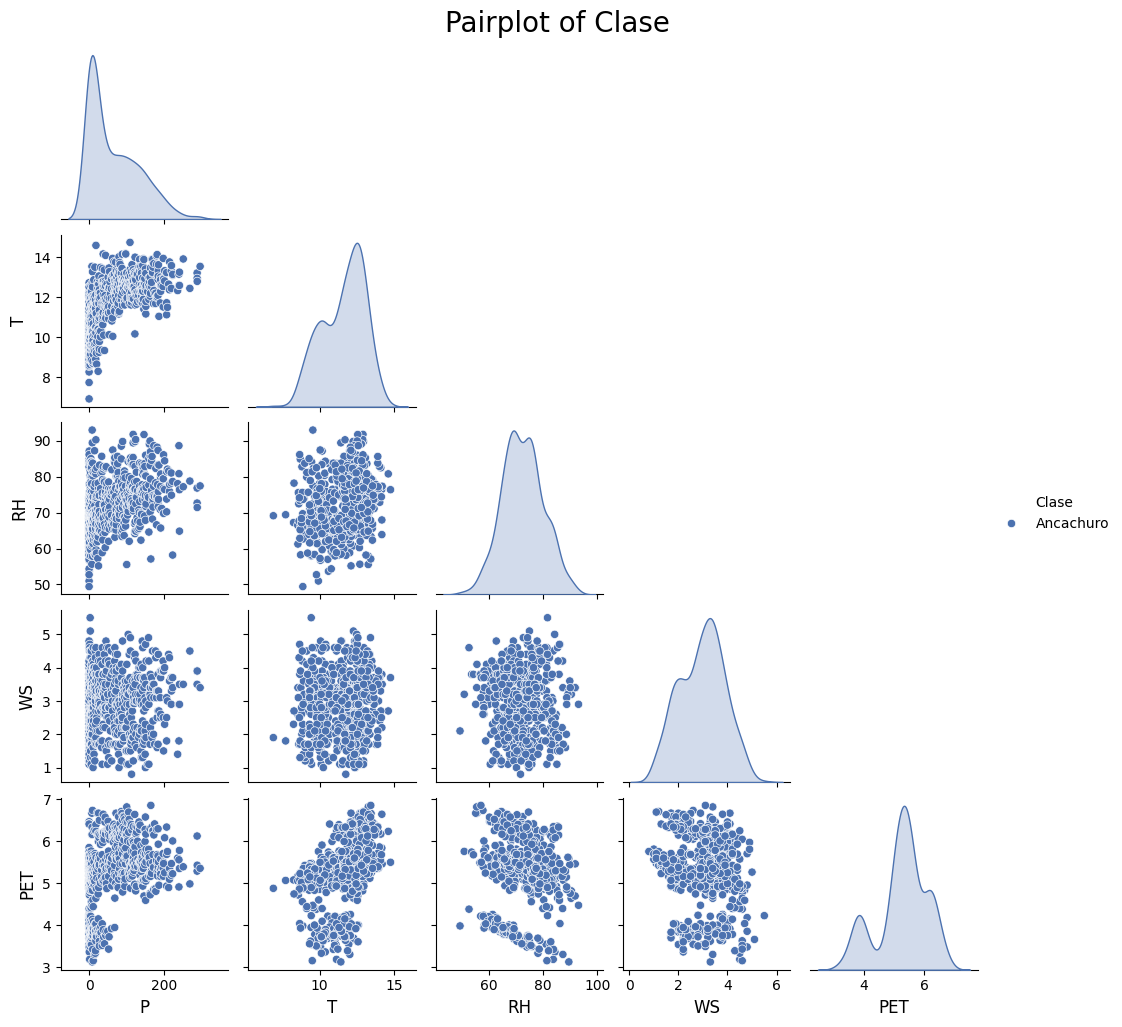
\includegraphics[width=0.45\textwidth]{resultados/por_estacion_meteorologica/Ancachuro/pairplot.png}
\caption{Pairplot de las variables meteorológicas en la estación Ancachuro.}
\label{fig:ancachuro_pairplot}
\end{figure}
\textbf{Interpretación:} El pairplot evidencia patrones visuales similares a los encontrados en la matriz de correlación. Se destaca la asociación positiva entre T y PET, y una relación moderada entre P y T. RH y WS presentan distribuciones dispersas respecto a las demás variables.





\section{Análisis Estadístico de la Estación Caraveli}

A continuación, se presenta el análisis estadístico descriptivo y exploratorio correspondiente a la estación meteorológica de Caraveli. Este incluye medidas univariadas por variable y relaciones bivariadas, junto con sus respectivas representaciones gráficas.

\subsection{Estadísticas Descriptivas}

\begin{table}[H]
\centering
\caption{Estadísticas descriptivas de las variables meteorológicas en la estación Caraveli}
\label{tab:stat_caraveli}
\tiny
\begin{tabular}{lrrrrr}
\toprule
\textbf{Estadístico} & \textbf{P (mm)} & \textbf{RH (\%)} & \textbf{T (°C)} & \textbf{WS (m/s)} & \textbf{PET (mm)} \\
\midrule
$n$    & 648.00 & 648.00 & 648.00 & 648.00 & 648.00 \\
Minimum                 & 0.00   & 32.21  & 16.74  & 0.50   & 5.84   \\
1st Quartile          & 0.00   & 47.02  & 19.05  & 1.90   & 7.07   \\
Median               & 0.00   & 54.46  & 19.78  & 2.20   & 7.50   \\
Mean                 & 2.92   & 54.76  & 19.76  & 2.31   & 7.49   \\
3rd Quartile           & 1.60   & 62.84  & 20.51  & 2.60   & 7.95   \\
Maximum                & 89.90  & 82.71  & 23.50  & 4.80   & 9.07   \\
Range                 & 89.90  & 50.50  & 6.76   & 4.00   & 3.23   \\
Interquartile Range  & 1.60   & 15.81  & 1.46   & 0.70   & 0.59   \\
Variance            & 67.75  & 120.56 & 1.08   & 0.32   & 0.38   \\
Standard Deviation          & 8.23   & 10.58  & 1.04   & 0.56   & 0.51   \\
Coefficient of Variation      & 2.82   & 0.20   & 0.05   & 0.24   & 0.08   \\
Skewness            & 5.65   & 0.13   & 0.14   & 0.56   & -0.13  \\
Kurtosis              & 42.79  & -0.53  & 0.07   & 1.07   & -0.39  \\
\bottomrule
\end{tabular}
\end{table}

\textbf{Interpretación:} La precipitación (P) en Caraveli es muy baja en la mayoría de los casos, con una fuerte Skewnesspositiva, lo que indica la presencia de eventos extremos aislados. La humedad relativa (RH) y la temperatura (T) se distribuyen de manera moderadamente simétrica, aunque con valores ligeramente variables. La velocidad del viento (WS) y la evapotranspiración potencial (PET) presentan una distribución estable con ligera variabilidad.

\subsection{Análisis Univariado}

\subsubsection*{Precipitación (P)}
\begin{figure}[H]
\centering
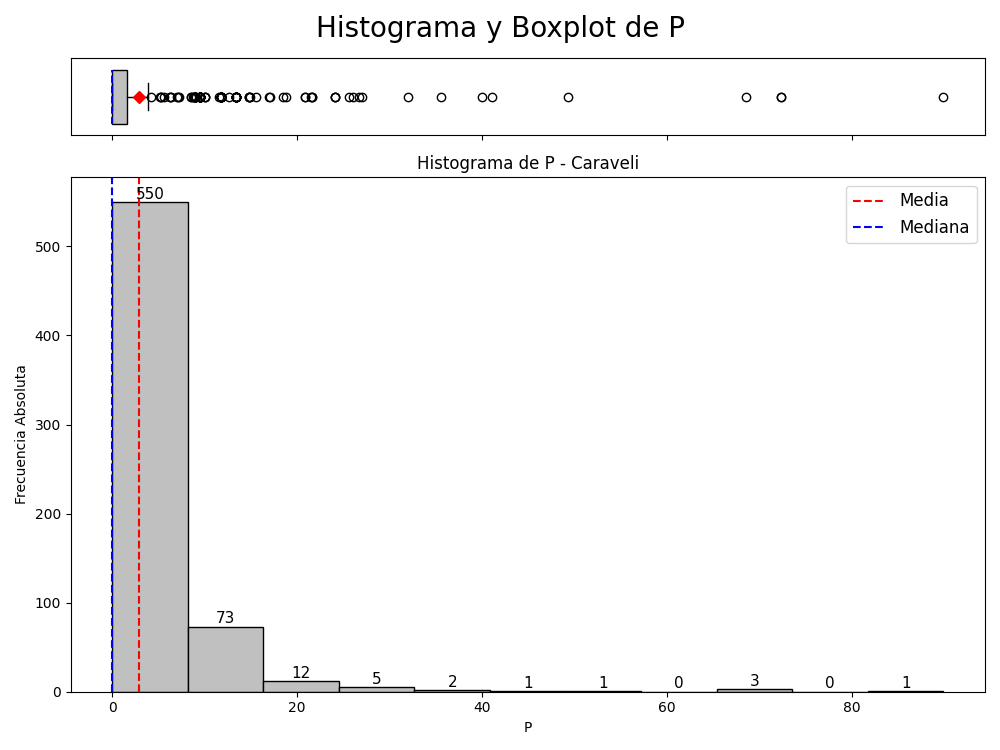
\includegraphics[width=0.4\textwidth]{resultados/por_estacion_meteorologica/Caraveli/P_histograma.png}
\caption{Histograma y boxplot de la precipitación (P) en la estación Caraveli.}
\label{fig:caraveli_P}
\end{figure}
\textbf{Interpretación:} La mayoría de los registros se concentran en cero milímetros, con pocos eventos de lluvia. La distribución es fuertemente sesgada a la derecha, con una Mean considerablemente superior a la mediana.

\subsubsection*{Temperatura (T)}
\begin{figure}[H]
\centering
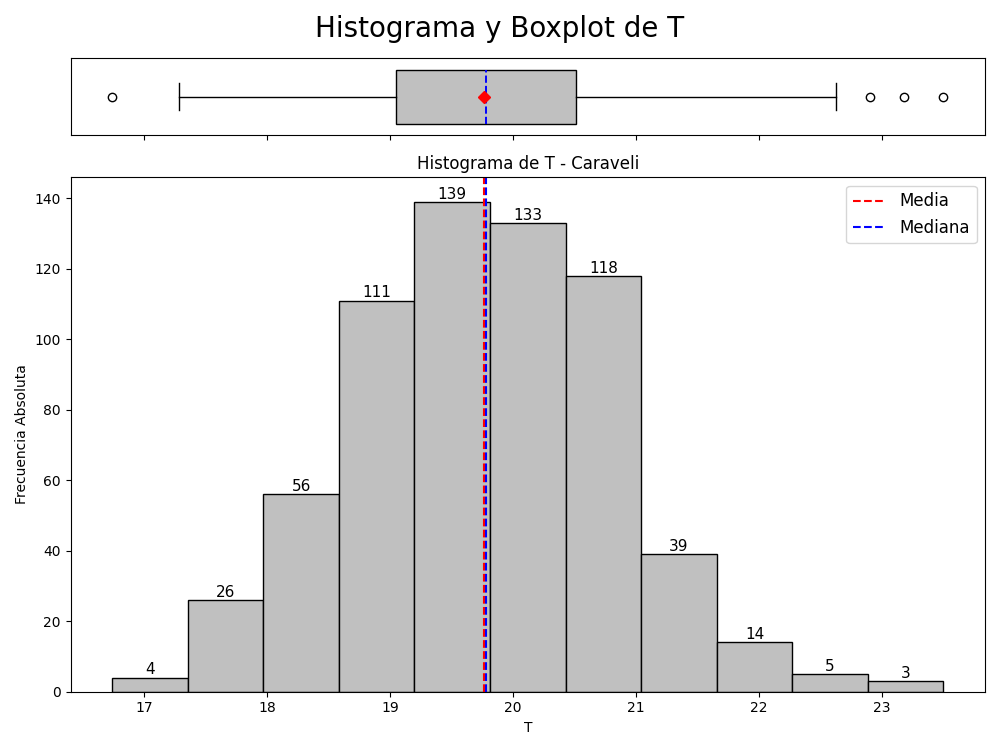
\includegraphics[width=0.4\textwidth]{resultados/por_estacion_meteorologica/Caraveli/T_histograma.png}
\caption{Histograma y boxplot de la temperatura (T) en la estación Caraveli.}
\label{fig:caraveli_T}
\end{figure}
\textbf{Interpretación:} La temperatura se distribuye de manera bastante simétrica, centrada en torno a los 20°C, con ligera dispersión hacia ambos extremos.

\subsubsection*{Humedad Relativa (RH)}
\begin{figure}[H]
\centering
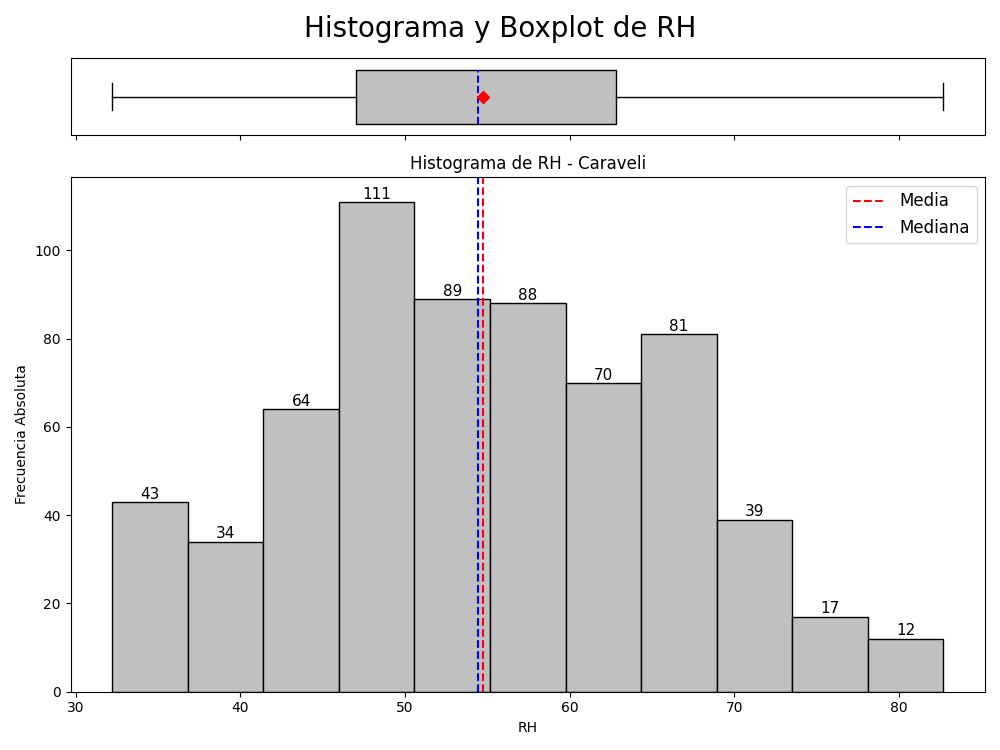
\includegraphics[width=0.4\textwidth]{resultados/por_estacion_meteorologica/Caraveli/RH_histograma.png}
\caption{Histograma y boxplot de la humedad relativa (RH) en la estación Caraveli.}
\label{fig:caraveli_RH}
\end{figure}
\textbf{Interpretación:} La RH muestra una distribución algo simétrica, con un Range amplio que abarca desde valores por debajo del 40\% hasta más del 80\%.

\subsubsection*{Velocidad del Viento (WS)}
\begin{figure}[H]
\centering
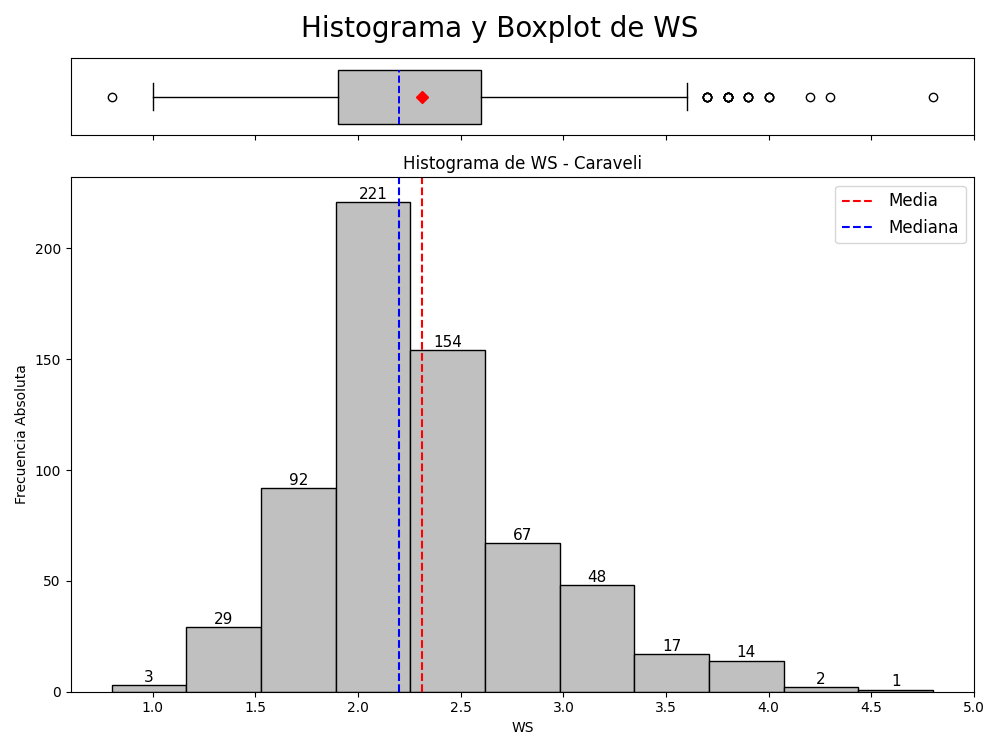
\includegraphics[width=0.4\textwidth]{resultados/por_estacion_meteorologica/Caraveli/WS_histograma.png}
\caption{Histograma y boxplot de la velocidad del viento (WS) en la estación Caraveli.}
\label{fig:caraveli_WS}
\end{figure}
\textbf{Interpretación:} La velocidad del viento se concentra principalmente entre 1.5 y 3.0 m/s. Se observan algunos valores atípicos por encima de 4.5 m/s.

\subsubsection*{Evapotranspiración Potencial (PET)}
\begin{figure}[H]
\centering
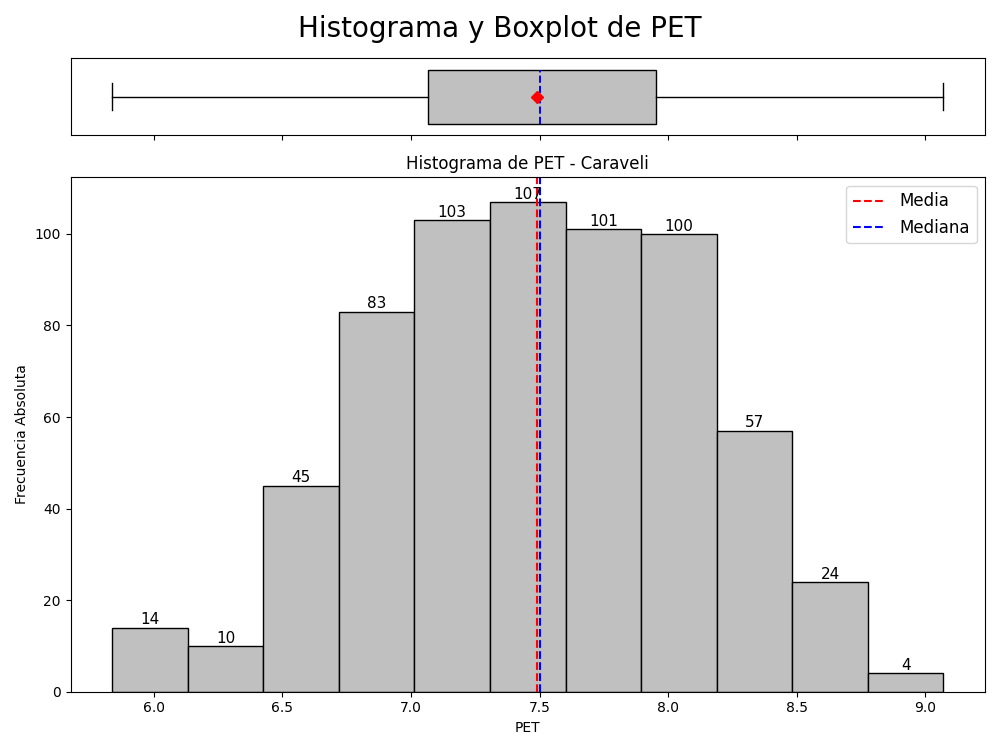
\includegraphics[width=0.4\textwidth]{resultados/por_estacion_meteorologica/Caraveli/PET_histograma.png}
\caption{Histograma y boxplot de la evapotranspiración potencial (PET) en la estación Caraveli.}
\label{fig:caraveli_PET}
\end{figure}
\textbf{Interpretación:} La PET se concentra en torno a 7.5 mm, mostrando una distribución relativamente simétrica y una baja variabilidad.

\subsection{Análisis Bivariado}

\subsubsection*{Matriz de Correlación}
\begin{figure}[H]
\centering
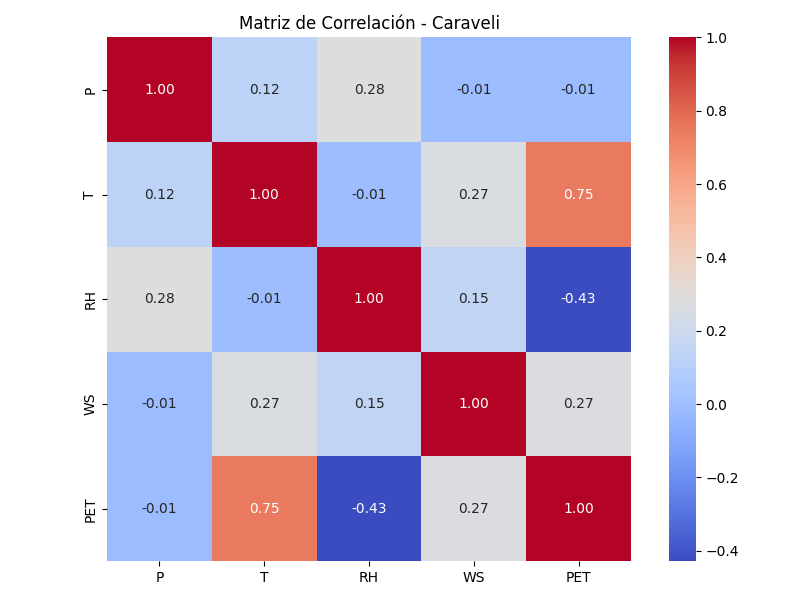
\includegraphics[width=0.4\textwidth]{resultados/por_estacion_meteorologica/Caraveli/matriz_correlacion.png}
\caption{Matriz de correlación de las variables meteorológicas en Caraveli.}
\label{fig:caraveli_corr}
\end{figure}
\textbf{Interpretación:} Se observa una fuerte correlación entre temperatura (T) y evapotranspiración (PET) (r = 0.75). La RH presenta una correlación negativa con PET (r = -0.43). El resto de las correlaciones son débiles o moderadas.

\subsubsection*{Gráfico de Pares (Pairplot)}
\begin{figure}[H]
\centering
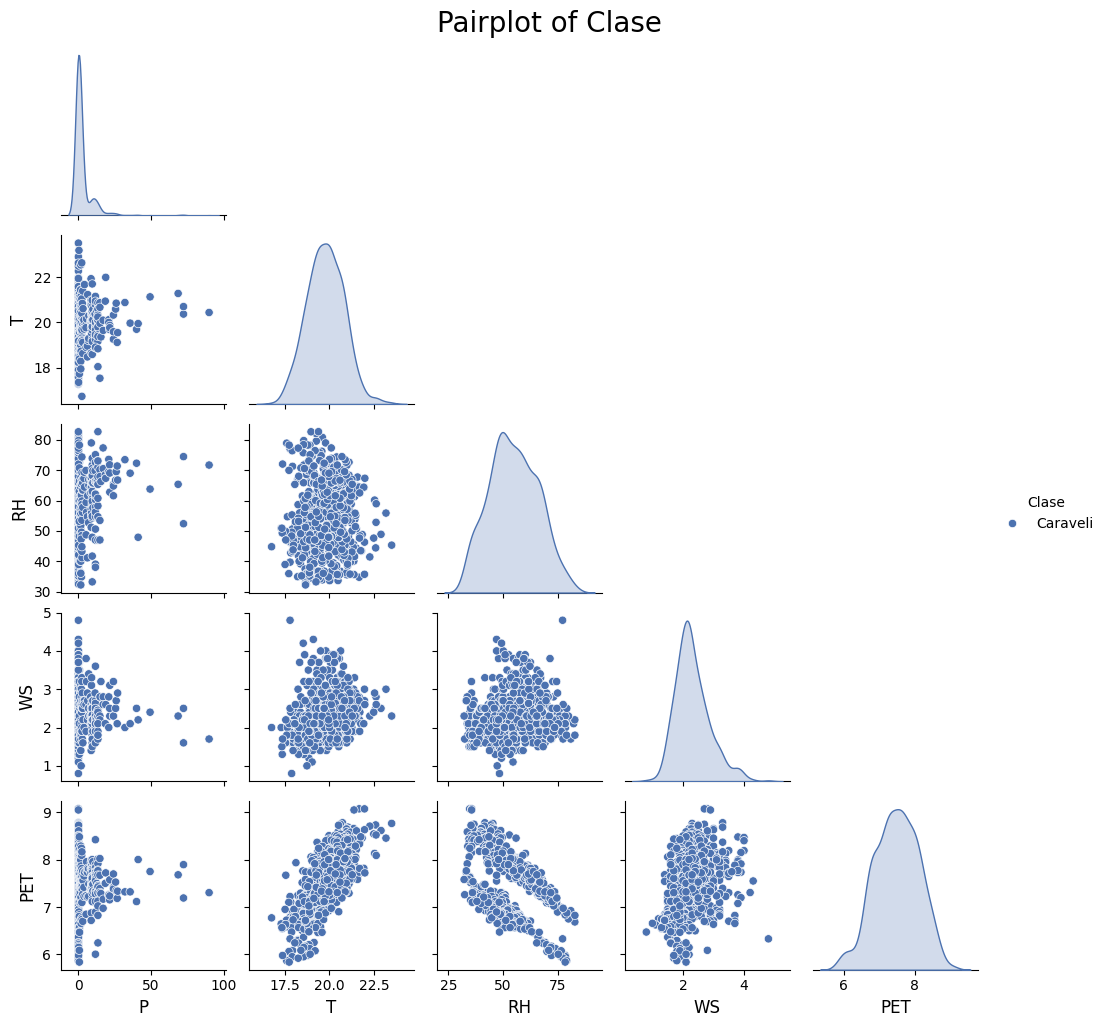
\includegraphics[width=0.45\textwidth]{resultados/por_estacion_meteorologica/Caraveli/pairplot.png}
\caption{Pairplot de las variables meteorológicas en la estación Caraveli.}
\label{fig:caraveli_pairplot}
\end{figure}
\textbf{Interpretación:} Se confirma visualmente la asociación positiva entre T y PET. Se detecta una leve relación negativa entre RH y PET. Las demás combinaciones no muestran patrones evidentes de asociación.




\section{Análisis Estadístico de la Estación Coracora}

A continuación se presenta el análisis estadístico descriptivo y exploratorio de la estación meteorológica de Coracora, considerando estadísticas univariadas y relaciones bivariadas con representaciones gráficas correspondientes.

\subsection{Estadísticas Descriptivas}

\begin{table}[H]
\centering
\caption{Descriptive statistics of meteorological variables at the Coracora station}
\label{tab:stat_coracora}
\tiny
\begin{tabular}{lrrrrr}
\toprule
\textbf{Statistic} & \textbf{P (mm)} & \textbf{RH (\%)} & \textbf{T (\textdegree C)} & \textbf{WS (m/s)} & \textbf{PET (mm)} \\
\midrule
$n$        & 648.00 & 648.00 & 648.00 & 648.00 & 648.00 \\
Minimum                 & 0.00 & 37.02 & 9.11 & 0.00 & 3.36 \\
1st Quartile            & 0.00 & 56.87 & 10.59 & 1.40 & 5.18 \\
Median                  & 6.82 & 68.44 & 11.78 & 1.90 & 5.57 \\
Mean                    & 36.94 & 67.40 & 11.82 & 2.03 & 5.52 \\
3rd Quartile            & 51.63 & 77.81 & 12.82 & 2.27 & 5.97 \\
Maximum                 & 382.70 & 90.51 & 15.00 & 15.40 & 7.23 \\
Range                   & 382.70 & 53.89 & 5.89 & 15.40 & 3.88 \\
Interquartile Range     & 51.63 & 20.54 & 1.93 & 0.57 & 0.50 \\
Variance                & 3399.42 & 170.53 & 1.39 & 1.70 & 0.57 \\
Standard Deviation      & 58.30 & 13.07 & 1.18 & 1.30 & 0.52 \\
Coefficient of Variation& 1.58 & 0.19 & 0.10 & 0.54 & 0.15 \\
Skewness              & 2.08 & -0.19 & 0.01 & 6.16 & -0.39 \\
Kurtosis                & 5.00 & -0.59 & -0.73 & 51.93 & -0.36 \\
\bottomrule
\end{tabular}
\end{table}

\textbf{Interpretación:} La precipitación presenta una Skewnesspositiva marcada y elevada dispersión, lo que indica eventos extremos de lluvia. La humedad relativa tiene una distribución relativamente simétrica. La temperatura está centrada en torno a 11.8 \textdegree C con baja dispersión. La velocidad del viento muestra valores extremos, mientras que la evapotranspiración potencial tiene una distribución simétrica y concentrada.

\subsection{Análisis Univariado}

\subsubsection*{Precipitación (P)}
\begin{figure}[H]
\centering
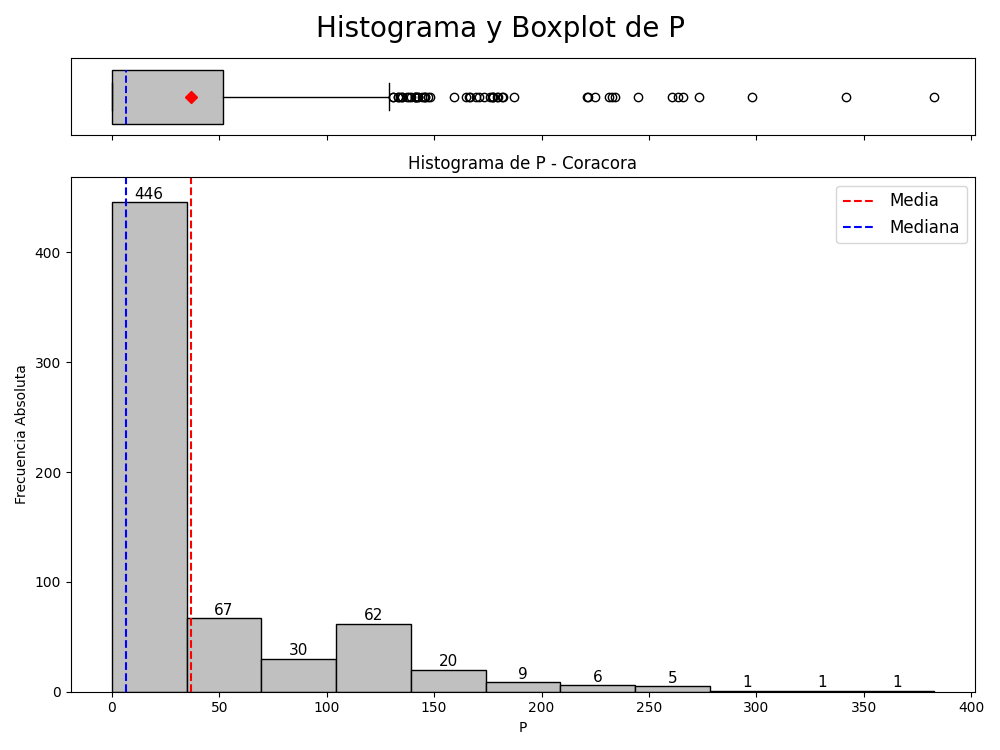
\includegraphics[width=0.4\textwidth]{resultados/por_estacion_meteorologica/Coracora/P_histograma.png}
\caption{Histograma y boxplot de la precipitación (P) en la estación Coracora.}
\label{fig:coracora_P}
\end{figure}
\textbf{Interpretación:} Distribución extremadamente sesgada a la derecha, con gran número de valores bajos y presencia de eventos extremos.

\subsubsection*{Temperatura (T)}
\begin{figure}[H]
\centering
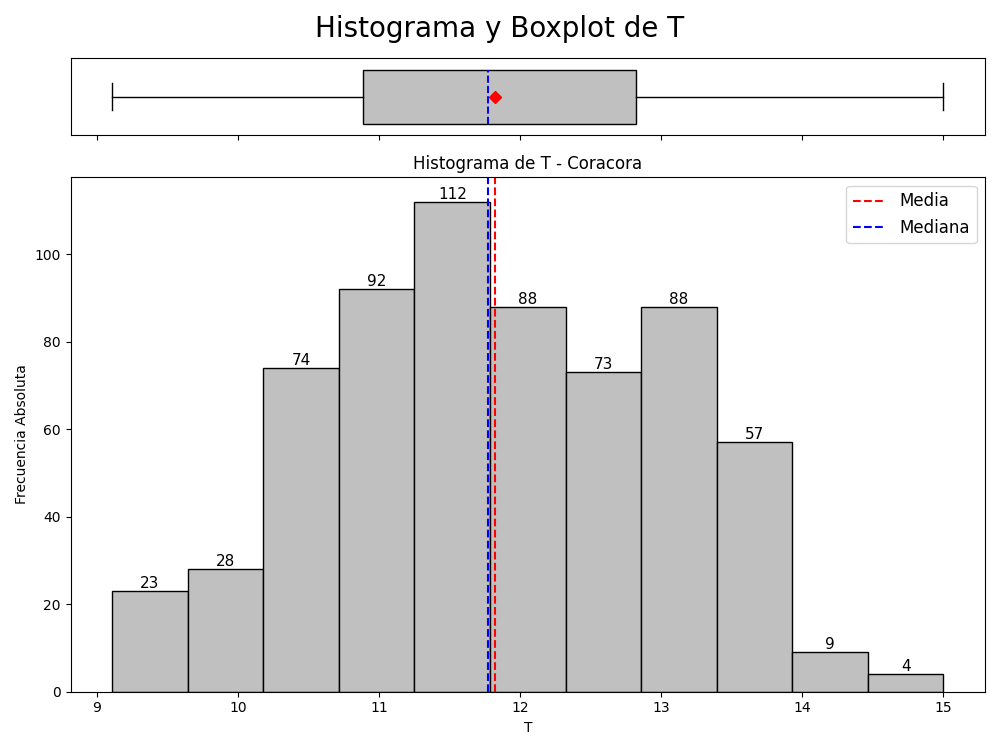
\includegraphics[width=0.4\textwidth]{resultados/por_estacion_meteorologica/Coracora/T_histograma.png}
\caption{Histograma y boxplot de la temperatura (T) en la estación Coracora.}
\label{fig:coracora_T}
\end{figure}
\textbf{Interpretación:} La distribución es simétrica con leve tendencia positiva. La mayoría de los valores se encuentran entre 10 y 13 \textdegree C.

\subsubsection*{Humedad Relativa (RH)}
\begin{figure}[H]
\centering
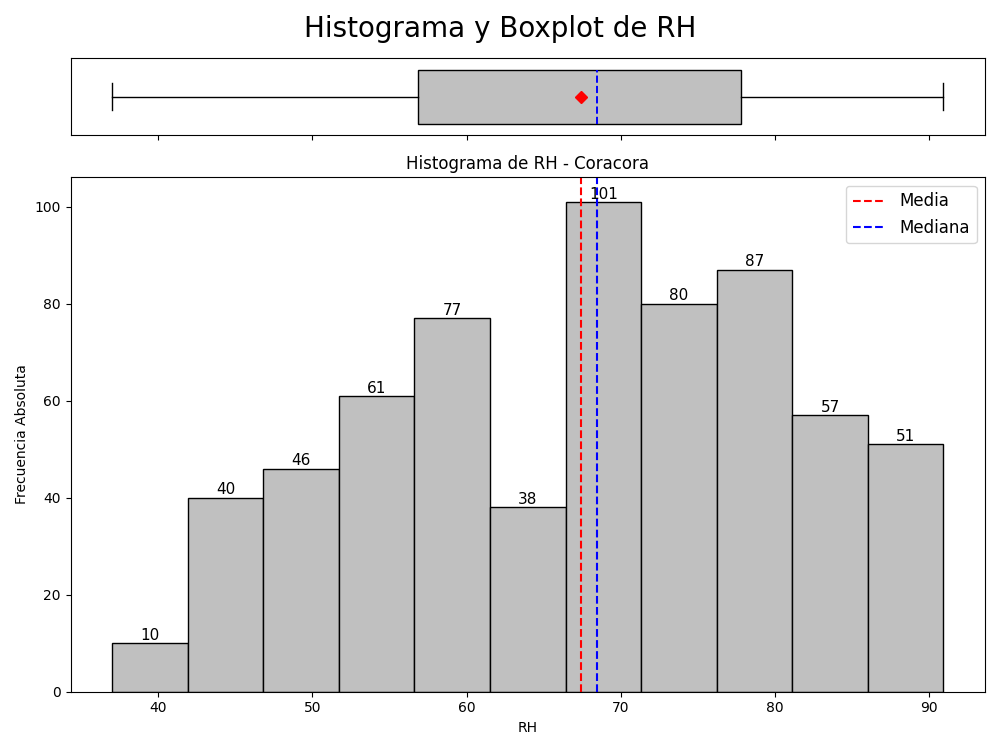
\includegraphics[width=0.4\textwidth]{resultados/por_estacion_meteorologica/Coracora/RH_histograma.png}
\caption{Histograma y boxplot de la humedad relativa (RH) en la estación Coracora.}
\label{fig:coracora_RH}
\end{figure}
\textbf{Interpretación:} Distribución amplia con valores que oscilan entre 40\% y 90\%. Ligera Skewnessnegativa.

\subsubsection*{Velocidad del Viento (WS)}
\begin{figure}[H]
\centering
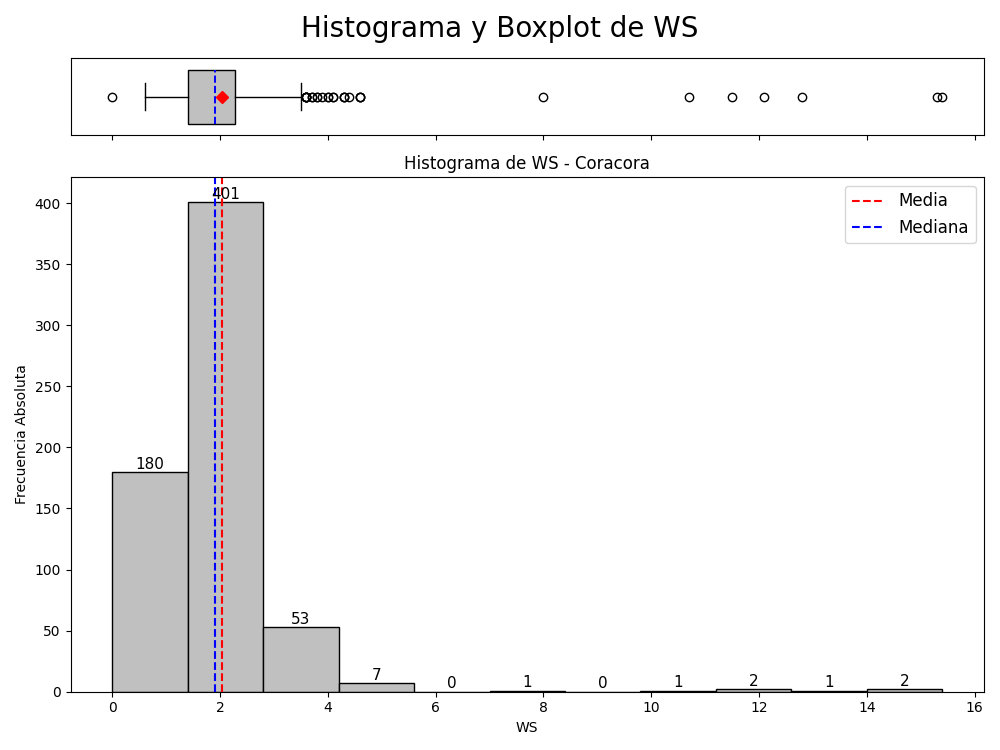
\includegraphics[width=0.4\textwidth]{resultados/por_estacion_meteorologica/Coracora/WS_histograma.png}
\caption{Histograma y boxplot de la velocidad del viento (WS) en la estación Coracora.}
\label{fig:coracora_WS}
\end{figure}
\textbf{Interpretación:} La mayor parte de los valores se concentran entre 1 y 3 m/s, con presencia de valores extremos hasta 15 m/s.

\subsubsection*{Evapotranspiración Potencial (PET)}
\begin{figure}[H]
\centering
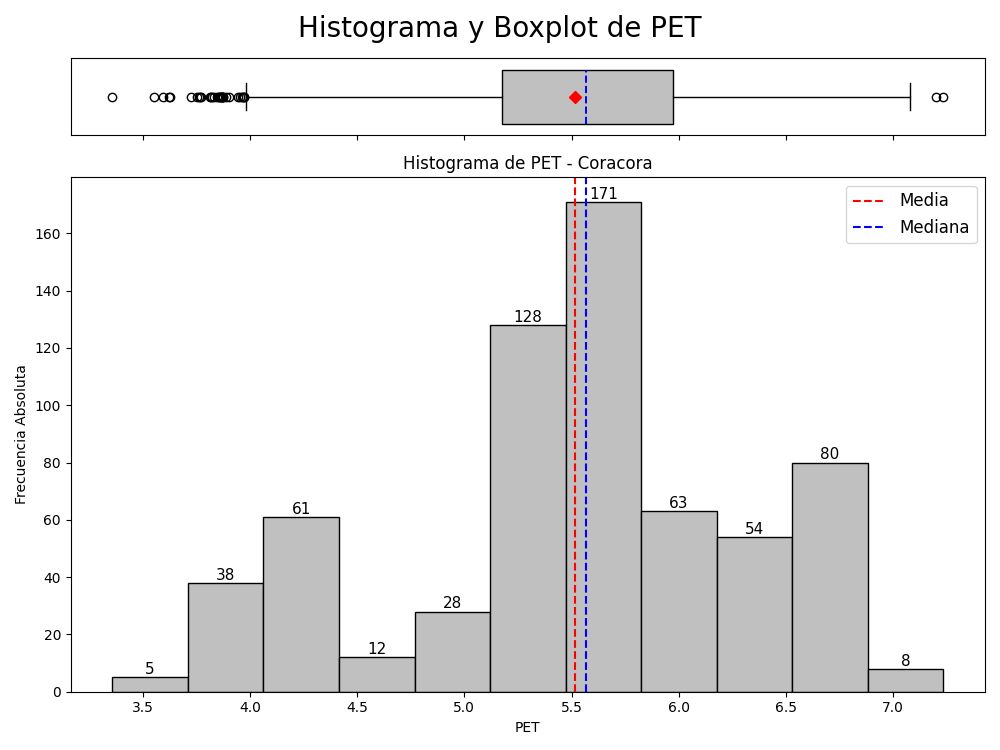
\includegraphics[width=0.4\textwidth]{resultados/por_estacion_meteorologica/Coracora/PET_histograma.png}
\caption{Histograma y boxplot de la evapotranspiración potencial (PET) en la estación Coracora.}
\label{fig:coracora_PET}
\end{figure}
\textbf{Interpretación:} Distribución simétrica con ligera Skewnessnegativa. La mayoría de valores están centrados entre 5 y 6 mm.

\subsection{Análisis Bivariado}

\subsubsection*{Matriz de Correlación}
\begin{figure}[H]
\centering
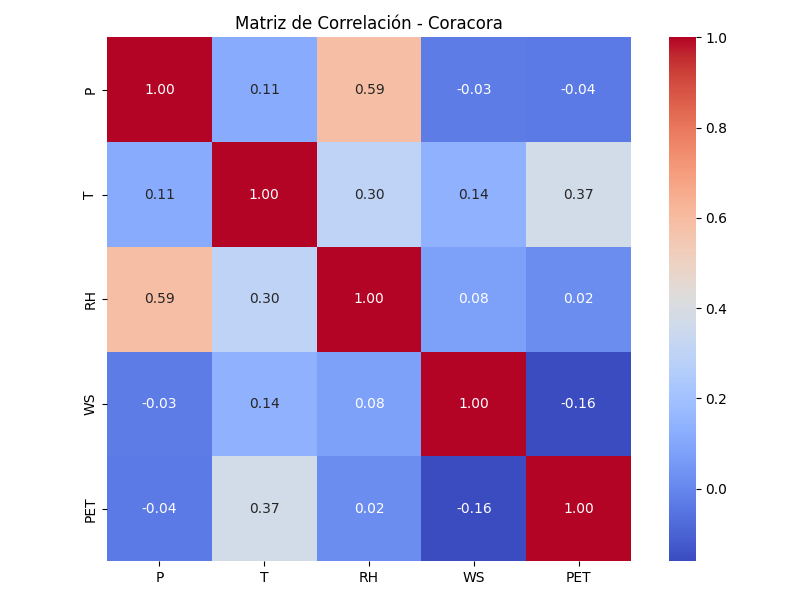
\includegraphics[width=0.4\textwidth]{resultados/por_estacion_meteorologica/Coracora/matriz_correlacion.png}
\caption{Matriz de correlación de las variables meteorológicas en Coracora.}
\label{fig:coracora_corr}
\end{figure}
\textbf{Interpretación:} Se observan correlaciones moderadas entre precipitación y humedad relativa ($r = 0.59$), y entre temperatura y PET ($r = 0.37$). El resto de las correlaciones son bajas.

\subsubsection*{Gráfico de Pares (Pairplot)}
\begin{figure}[H]
\centering
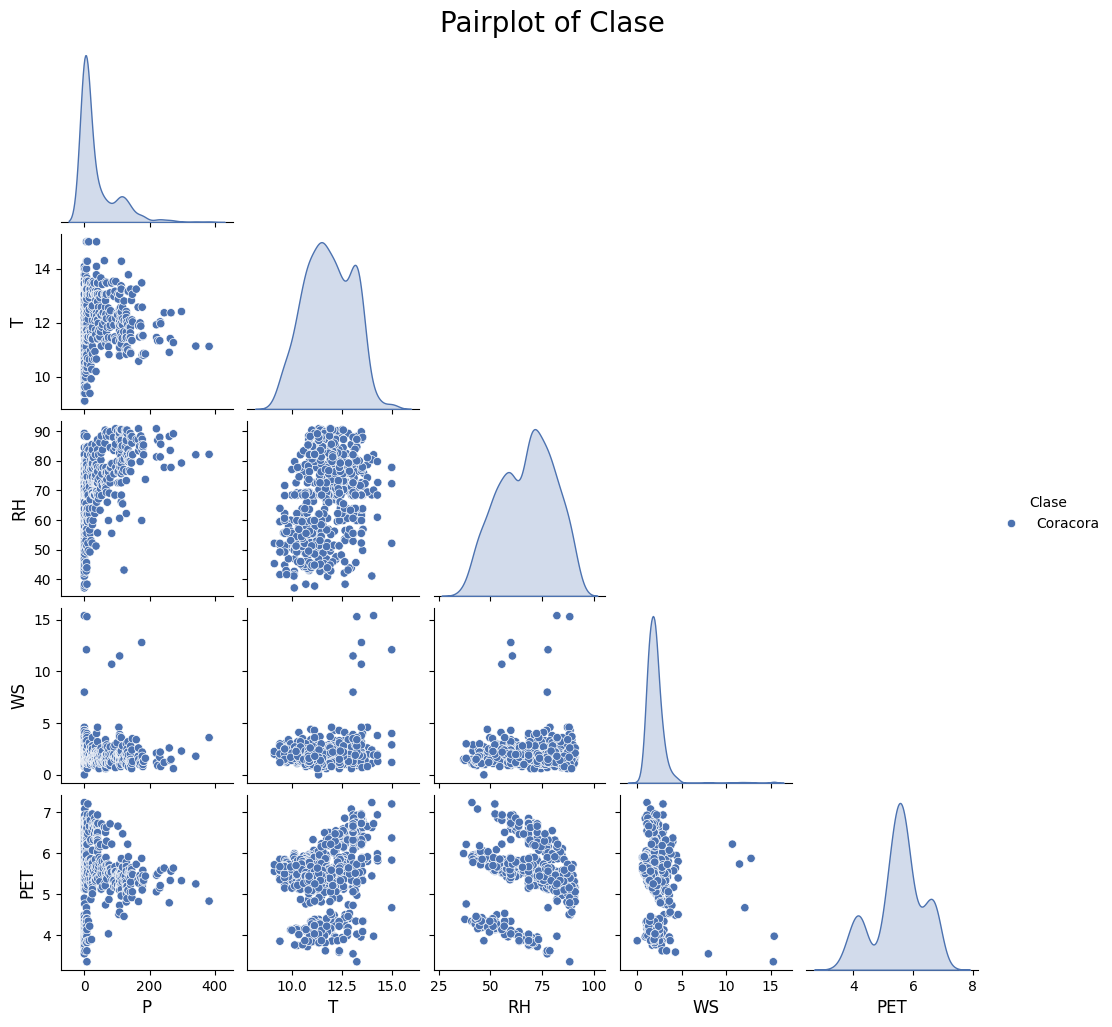
\includegraphics[width=0.45\textwidth]{resultados/por_estacion_meteorologica/Coracora/pairplot.png}
\caption{Pairplot de las variables meteorológicas en la estación Coracora.}
\label{fig:coracora_pairplot}
\end{figure}
\textbf{Interpretación:} Se confirman visualmente las correlaciones observadas. Se destacan patrones lineales entre T y PET, y agrupaciones densas en la distribución de P, RH y WS.





\section{Análisis Estadístico de la Estación Cotahuasi}

A continuación se presenta el análisis estadístico descriptivo y exploratorio de la estación meteorológica de Cotahuasi, considerando estadísticas univariadas y relaciones bivariadas con representaciones gráficas correspondientes.

\subsection{Estadísticas Descriptivas}

\begin{table}[H]
\centering
\caption{Estadísticas descriptivas de las variables meteorológicas en la estación Cotahuasi}
\label{tab:stat_cotahuasi}
\tiny
\begin{tabular}{lrrrrr}
\toprule
\textbf{Estadístico} & \textbf{P (mm)} & \textbf{RH (\%)} & \textbf{T (\textdegree C)} & \textbf{WS (m/s)} & \textbf{PET (mm)} \\
\midrule
$n$                  & 648.00 & 648.00 & 648.00 & 648.00 & 648.00 \\
Minimum                 & 0.00 & 28.01 & 13.66 & 1.20 & 5.78 \\
1st Quartile          & 0.00 & 38.85 & 15.14 & 2.90 & 6.78 \\
Median               & 4.25 & 47.88 & 15.82 & 3.30 & 7.14 \\
Mean                 & 26.38 & 51.29 & 15.91 & 3.40 & 7.22 \\
3rd Quartile           & 32.53 & 63.26 & 16.60 & 3.70 & 7.62 \\
Maximum                & 205.40 & 83.61 & 20.33 & 11.10 & 8.83 \\
Range                 & 205.40 & 55.60 & 6.67 & 9.90 & 3.05 \\
Interquartile Range  & 32.53 & 24.41 & 1.47 & 0.50 & 0.54 \\
Variance            & 1744.29 & 208.17 & 1.11 & 1.46 & 0.37 \\
Standard Deviation          & 41.76 & 14.43 & 1.05 & 1.21 & 0.51 \\
Coefficient of Variation      & 1.58 & 0.28 & 0.07 & 0.36 & 0.08 \\
Skewness            & 1.88 & 0.44 & 0.57 & 3.36 & 0.40 \\
Kurtosis              & 2.96 & -1.06 & 0.33 & 16.03 & -0.50 \\
\bottomrule
\end{tabular}
\end{table}

\textbf{Interpretación:} La precipitación muestra una distribución fuertemente sesgada a la derecha con valores extremos significativos. La humedad relativa es más variable, con Skewnessmoderada positiva. La temperatura es bastante homogénea. La velocidad del viento presenta Kurtosis alta por eventos atípicos. La evapotranspiración potencial muestra distribución levemente sesgada.

\subsection{Análisis Univariado}

\subsubsection*{Precipitación (P)}
\begin{figure}[H]
\centering
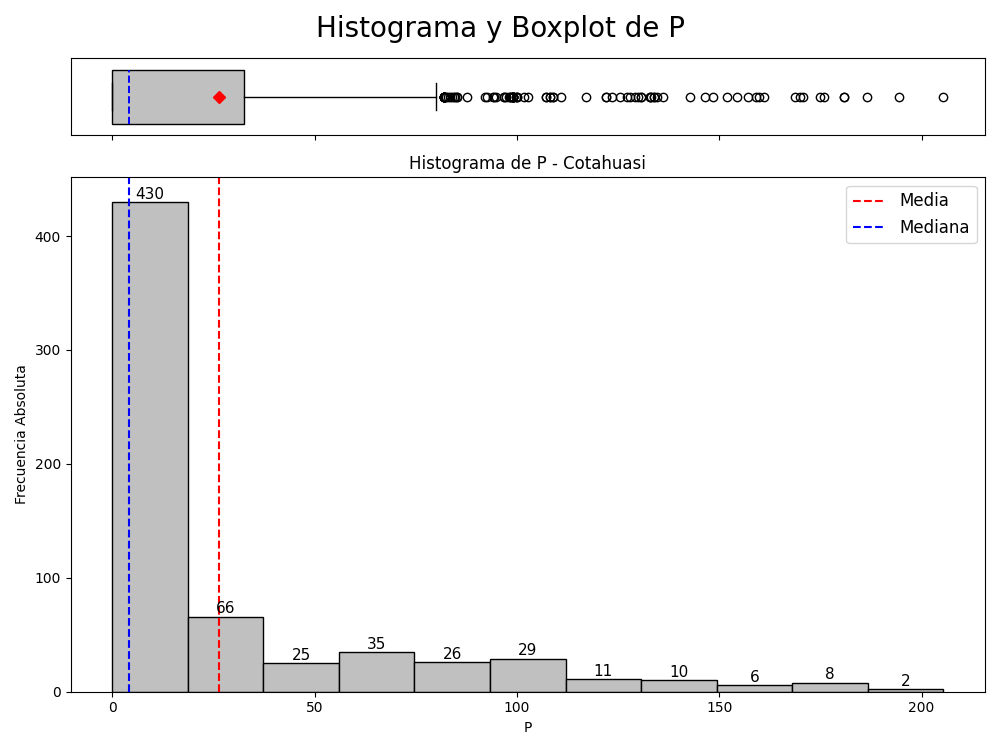
\includegraphics[width=0.4\textwidth]{resultados/por_estacion_meteorologica/Cotahuasi/P_histograma.png}
\caption{Histograma y boxplot de la precipitación (P) en la estación Cotahuasi.}
\label{fig:cotahuasi_P}
\end{figure}
\textbf{Interpretación:} Alta frecuencia de valores bajos de precipitación, pero con varios eventos extremos, reflejando una distribución sesgada positiva.

\subsubsection*{Temperatura (T)}
\begin{figure}[H]
\centering
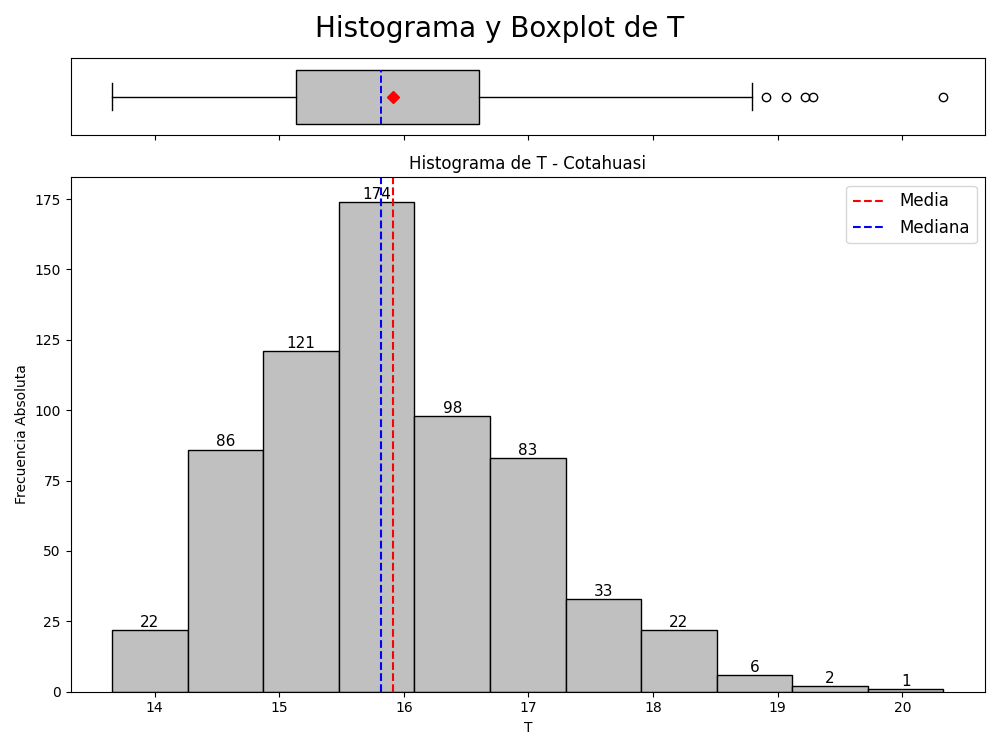
\includegraphics[width=0.4\textwidth]{resultados/por_estacion_meteorologica/Cotahuasi/T_histograma.png}
\caption{Histograma y boxplot de la temperatura (T) en la estación Cotahuasi.}
\label{fig:cotahuasi_T}
\end{figure}
\textbf{Interpretación:} La distribución es simétrica y estrecha. La mayoría de los valores oscilan entre 15 y 17 \textdegree C.

\subsubsection*{Humedad Relativa (RH)}
\begin{figure}[H]
\centering
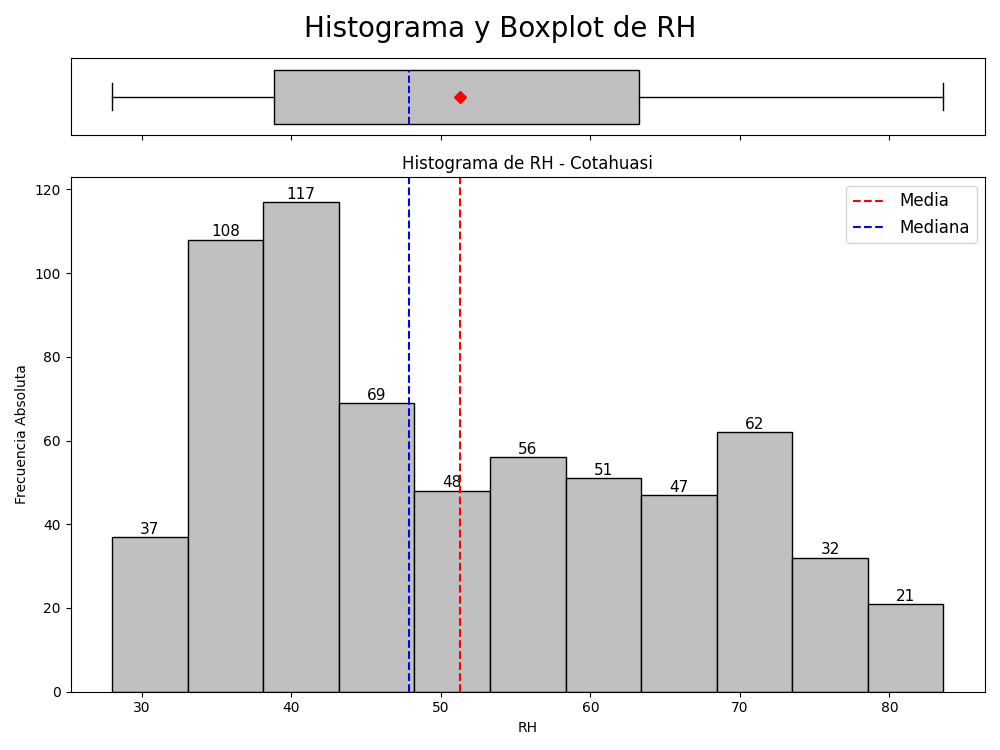
\includegraphics[width=0.4\textwidth]{resultados/por_estacion_meteorologica/Cotahuasi/RH_histograma.png}
\caption{Histograma y boxplot de la humedad relativa (RH) en la estación Cotahuasi.}
\label{fig:cotahuasi_RH}
\end{figure}
\textbf{Interpretación:} Distribución amplia con dispersión significativa. Predominan valores entre 40\% y 70\%.

\subsubsection*{Velocidad del Viento (WS)}
\begin{figure}[H]
\centering
\includegraphics[width=0.4\textwidth]{resultados/por_estacion_meteorologica/Cotahuasi/WS_histograma.png}
\caption{Histograma y boxplot de la velocidad del viento (WS) en la estación Cotahuasi.}
\label{fig:cotahuasi_WS}
\end{figure}
\textbf{Interpretación:} La mayoría de los datos se encuentran entre 2.5 y 4 m/s. Se evidencian varios valores atípicos que alcanzan hasta 11 m/s.

\subsubsection*{Evapotranspiración Potencial (PET)}
\begin{figure}[H]
\centering
\includegraphics[width=0.4\textwidth]{resultados/por_estacion_meteorologica/Cotahuasi/PET_histograma.png}
\caption{Histograma y boxplot de la evapotranspiración potencial (PET) en la estación Cotahuasi.}
\label{fig:cotahuasi_PET}
\end{figure}
\textbf{Interpretación:} Distribución ligeramente sesgada a la derecha. La mayoría de los valores oscilan entre 6.5 y 8 mm.

\subsection{Análisis Bivariado}

\subsubsection*{Matriz de Correlación}
\begin{figure}[H]
\centering
\includegraphics[width=0.4\textwidth]{resultados/por_estacion_meteorologica/Cotahuasi/matriz_correlacion.png}
\caption{Matriz de correlación de las variables meteorológicas en Cotahuasi.}
\label{fig:cotahuasi_corr}
\end{figure}
\textbf{Interpretación:} Se observa una alta correlación positiva entre P y RH (r = 0.76), así como entre T y PET (r = 0.51). La correlación entre RH y PET es negativa (r = -0.52), sugiriendo que a menor humedad, mayor es la evapotranspiración potencial.

\subsubsection*{Gráfico de Pares (Pairplot)}
\begin{figure}[H]
\centering
\includegraphics[width=0.45\textwidth]{resultados/por_estacion_meteorologica/Cotahuasi/pairplot.png}
\caption{Pairplot de las variables meteorológicas en la estación Cotahuasi.}
\label{fig:cotahuasi_pairplot}
\end{figure}
\textbf{Interpretación:} El gráfico confirma las asociaciones observadas: fuerte relación lineal entre T y PET, y entre P y RH. También se observan distribuciones densas y patrones consistentes con las correlaciones.




\section{Análisis Estadístico de la Estación Cotahuasi}

A continuación se presenta el análisis estadístico descriptivo y exploratorio de la estación meteorológica de Cotahuasi, considerando estadísticas univariadas y relaciones bivariadas con representaciones gráficas correspondientes.

\subsection{Estadísticas Descriptivas}

\begin{table}[H]
\centering
\caption{Estadísticas descriptivas de las variables meteorológicas en la estación Cotahuasi}
\label{tab:stat_cotahuasi}
\tiny
\begin{tabular}{lrrrrr}
\toprule
\textbf{Estadístico} & \textbf{P (mm)} & \textbf{RH (\%)} & \textbf{T (\textdegree C)} & \textbf{WS (m/s)} & \textbf{PET (mm)} \\
\midrule
$n$  & 648.00 & 648.00 & 648.00 & 648.00 & 648.00 \\
Minimum                 & 0.00 & 28.01 & 13.66 & 1.20 & 5.78 \\
1st Quartile          & 0.00 & 38.85 & 15.14 & 2.90 & 6.78 \\
Median               & 4.25 & 47.88 & 15.82 & 3.30 & 7.14 \\
Mean                 & 26.38 & 51.29 & 15.91 & 3.40 & 7.22 \\
3rd Quartile           & 32.53 & 63.26 & 16.60 & 3.70 & 7.62 \\
Maximum                & 205.40 & 83.61 & 20.33 & 11.10 & 8.83 \\
Range                 & 205.40 & 55.60 & 6.67 & 9.90 & 3.05 \\
Interquartile Range  & 32.53 & 24.41 & 1.47 & 0.50 & 0.54 \\
Variance            & 1744.29 & 208.17 & 1.11 & 1.46 & 0.37 \\
Standard Deviation          & 41.76 & 14.43 & 1.05 & 1.21 & 0.51 \\
Coefficient of Variation      & 1.58 & 0.28 & 0.07 & 0.36 & 0.08 \\
Skewness            & 1.88 & 0.44 & 0.57 & 3.36 & 0.40 \\
Kurtosis              & 2.96 & -1.06 & 0.33 & 16.03 & -0.50 \\
\bottomrule
\end{tabular}
\end{table}

\textbf{Interpretación:} La precipitación muestra una distribución fuertemente sesgada a la derecha con valores extremos significativos. La humedad relativa es más variable, con Skewnessmoderada positiva. La temperatura es bastante homogénea. La velocidad del viento presenta Kurtosis alta por eventos atípicos. La evapotranspiración potencial muestra distribución levemente sesgada.

\subsection{Análisis Univariado}

\subsubsection*{Precipitación (P)}
\begin{figure}[H]
\centering
\includegraphics[width=0.4\textwidth]{resultados/por_estacion_meteorologica/Cotahuasi/P_histograma.png}
\caption{Histograma y boxplot de la precipitación (P) en la estación Cotahuasi.}
\label{fig:cotahuasi_P}
\end{figure}
\textbf{Interpretación:} Alta frecuencia de valores bajos de precipitación, pero con varios eventos extremos, reflejando una distribución sesgada positiva.

\subsubsection*{Temperatura (T)}
\begin{figure}[H]
\centering
\includegraphics[width=0.4\textwidth]{resultados/por_estacion_meteorologica/Cotahuasi/T_histograma.png}
\caption{Histograma y boxplot de la temperatura (T) en la estación Cotahuasi.}
\label{fig:cotahuasi_T}
\end{figure}
\textbf{Interpretación:} La distribución es simétrica y estrecha. La mayoría de los valores oscilan entre 15 y 17 \textdegree C.

\subsubsection*{Humedad Relativa (RH)}
\begin{figure}[H]
\centering
\includegraphics[width=0.4\textwidth]{resultados/por_estacion_meteorologica/Cotahuasi/RH_histograma.png}
\caption{Histograma y boxplot de la humedad relativa (RH) en la estación Cotahuasi.}
\label{fig:cotahuasi_RH}
\end{figure}
\textbf{Interpretación:} Distribución amplia con dispersión significativa. Predominan valores entre 40\% y 70\%.

\subsubsection*{Velocidad del Viento (WS)}
\begin{figure}[H]
\centering
\includegraphics[width=0.4\textwidth]{resultados/por_estacion_meteorologica/Cotahuasi/WS_histograma.png}
\caption{Histograma y boxplot de la velocidad del viento (WS) en la estación Cotahuasi.}
\label{fig:cotahuasi_WS}
\end{figure}
\textbf{Interpretación:} La mayoría de los datos se encuentran entre 2.5 y 4 m/s. Se evidencian varios valores atípicos que alcanzan hasta 11 m/s.

\subsubsection*{Evapotranspiración Potencial (PET)}
\begin{figure}[H]
\centering
\includegraphics[width=0.4\textwidth]{resultados/por_estacion_meteorologica/Cotahuasi/PET_histograma.png}
\caption{Histograma y boxplot de la evapotranspiración potencial (PET) en la estación Cotahuasi.}
\label{fig:cotahuasi_PET}
\end{figure}
\textbf{Interpretación:} Distribución ligeramente sesgada a la derecha. La mayoría de los valores oscilan entre 6.5 y 8 mm.

\subsection{Análisis Bivariado}

\subsubsection*{Matriz de Correlación}
\begin{figure}[H]
\centering
\includegraphics[width=0.4\textwidth]{resultados/por_estacion_meteorologica/Cotahuasi/matriz_correlacion.png}
\caption{Matriz de correlación de las variables meteorológicas en Cotahuasi.}
\label{fig:cotahuasi_corr}
\end{figure}
\textbf{Interpretación:} Se observa una alta correlación positiva entre P y RH (r = 0.76), así como entre T y PET (r = 0.51). La correlación entre RH y PET es negativa (r = -0.52), sugiriendo que a menor humedad, mayor es la evapotranspiración potencial.

\subsubsection*{Gráfico de Pares (Pairplot)}
\begin{figure}[H]
\centering
\includegraphics[width=0.45\textwidth]{resultados/por_estacion_meteorologica/Cotahuasi/pairplot.png}
\caption{Pairplot de las variables meteorológicas en la estación Cotahuasi.}
\label{fig:cotahuasi_pairplot}
\end{figure}
\textbf{Interpretación:} El gráfico confirma las asociaciones observadas: fuerte relación lineal entre T y PET, y entre P y RH. También se observan distribuciones densas y patrones consistentes con las correlaciones.




\section{Análisis Estadístico de la Estación Huambo}

A continuación se presenta el análisis estadístico descriptivo y exploratorio de la estación meteorológica de Huambo, considerando estadísticas univariadas y relaciones bivariadas con representaciones gráficas correspondientes.

\subsection{Estadísticas Descriptivas}

\begin{table}[H]
\centering
\caption{Estadísticas descriptivas de las variables meteorológicas en la estación Huambo}
\label{tab:stat_huambo}
\tiny
\begin{tabular}{lrrrrr}
\toprule
\textbf{Estadístico} & \textbf{P (mm)} & \textbf{RH (\%)} & \textbf{T (°C)} & \textbf{WS (m/s)} & \textbf{PET (mm)} \\
\midrule
$n$         & 648.00 & 648.00 & 648.00 & 648.00 & 648.00 \\
Minimum                         & 0.00   & 36.90  & 8.21   & 1.40   & 4.67   \\
1.er cuartil                 & 0.00   & 53.24  & 9.60   & 2.38   & 5.56   \\
Median                       & 2.50   & 60.15  & 10.34  & 3.00   & 5.91   \\
Mean                         & 22.67  & 62.80  & 10.31  & 3.01   & 5.91   \\
3.er cuartil                & 29.50  & 72.10  & 11.01  & 3.60   & 6.28   \\
Maximum                        & 186.90 & 88.40  & 13.14  & 4.50   & 7.07   \\
Range                         & 186.90 & 51.50  & 4.93   & 3.10   & 2.41   \\
Interquartile Range          & 29.50  & 18.86  & 1.41   & 1.23   & 0.72   \\
Variance                    & 1387.26& 147.53 & 1.05   & 0.52   & 0.22   \\
Desviación estándar           & 37.25  & 12.15  & 1.03   & 0.72   & 0.46   \\
Coeficiente de variación     & 1.64   & 0.19   & 0.10   & 0.24   & 0.08   \\
Skewness                    & 2.04   & 0.35   & 0.00   & 0.09   & -0.07  \\
Kurtosis                      & 3.89   & -0.51  & -0.47  & -1.10  & -0.73  \\
\bottomrule
\end{tabular}
\end{table}

\textbf{Interpretación:} La variable precipitación muestra alta Skewness positiva, indicando la presencia de eventos extremos. La temperatura presenta una distribución aproximadamente normal. La velocidad del viento tiene una distribución simétrica centrada en 3 m/s. La humedad relativa presenta un sesgo ligero hacia la izquierda. La PET está levemente sesgada hacia la izquierda y centrada alrededor de 5.9 mm.

\subsection{Análisis Univariado}

\subsubsection*{Precipitación (P)}
\begin{figure}[H]
\centering
\includegraphics[width=0.4\textwidth]{resultados/por_estacion_meteorologica/Huambo/P_histograma.png}
\caption{Histograma y boxplot de la precipitación (P) en la estación Huambo.}
\label{fig:huambo_P}
\end{figure}
\textbf{Interpretación:} Distribución fuertemente sesgada a la derecha con alta frecuencia de valores bajos y presencia de precipitaciones intensas puntuales.

\subsubsection*{Temperatura (T)}
\begin{figure}[H]
\centering
\includegraphics[width=0.4\textwidth]{resultados/por_estacion_meteorologica/Huambo/T_histograma.png}
\caption{Histograma y boxplot de la temperatura (T) en la estación Huambo.}
\label{fig:huambo_T}
\end{figure}
\textbf{Interpretación:} Distribución simétrica centrada entre 9 y 11 °C, con bajo nivel de dispersión.

\subsubsection*{Humedad Relativa (RH)}
\begin{figure}[H]
\centering
\includegraphics[width=0.4\textwidth]{resultados/por_estacion_meteorologica/Huambo/RH_histograma.png}
\caption{Histograma y boxplot de la humedad relativa (RH) en la estación Huambo.}
\label{fig:huambo_RH}
\end{figure}
\textbf{Interpretación:} Valores centrados entre 50\% y 70\%, con ligera Skewnesspositiva.

\subsubsection*{Velocidad del Viento (WS)}
\begin{figure}[H]
\centering
\includegraphics[width=0.4\textwidth]{resultados/por_estacion_meteorologica/Huambo/WS_histograma.png}
\caption{Histograma y boxplot de la velocidad del viento (WS) en la estación Huambo.}
\label{fig:huambo_WS}
\end{figure}
\textbf{Interpretación:} La distribución es simétrica, concentrada entre 2.5 y 3.5 m/s, sin valores extremos significativos.

\subsubsection*{Evapotranspiración Potencial (PET)}
\begin{figure}[H]
\centering
\includegraphics[width=0.4\textwidth]{resultados/por_estacion_meteorologica/Huambo/PET_histograma.png}
\caption{Histograma y boxplot de la evapotranspiración potencial (PET) en la estación Huambo.}
\label{fig:huambo_PET}
\end{figure}
\textbf{Interpretación:} Distribución simétrica con valores concentrados entre 5.5 y 6.5 mm.

\subsection{Análisis Bivariado}

\subsubsection*{Matriz de Correlación}
\begin{figure}[H]
\centering
\includegraphics[width=0.4\textwidth]{resultados/por_estacion_meteorologica/Huambo/matriz_correlacion.png}
\caption{Matriz de correlación de las variables meteorológicas en la estación Huambo.}
\label{fig:huambo_corr}
\end{figure}
\textbf{Interpretación:} Se evidencian correlaciones moderadas entre Precipitación y Humedad Relativa (r = 0.73), así como entre Temperatura y PET (r = 0.71). También hay correlaciones negativas moderadas entre RH y WS, y entre WS y PET.

\subsubsection*{Gráfico de Pares (Pairplot)}
\begin{figure}[H]
\centering
\includegraphics[width=0.45\textwidth]{resultados/por_estacion_meteorologica/Huambo/pairplot.png}
\caption{Pairplot de las variables meteorológicas en la estación Huambo.}
\label{fig:huambo_pairplot}
\end{figure}
\textbf{Interpretación:} Se aprecian relaciones lineales destacadas entre T y PET, así como entre P y RH. También se observa agrupamiento en las variables WS y T.



\section{Análisis Estadístico de la Estación Huaraya}

A continuación se presenta el análisis estadístico descriptivo y exploratorio de la estación meteorológica de Huaraya, considerando estadísticas univariadas y relaciones bivariadas con representaciones gráficas correspondientes.

\subsection{Estadísticas Descriptivas}

\begin{table}[H]
\centering
\caption{Estadísticas descriptivas de las variables meteorológicas en la estación Huaraya}
\label{tab:stat_huaraya}
\tiny
\begin{tabular}{lrrrrr}
\toprule
\textbf{Estadístico} & \textbf{P (mm)} & \textbf{RH (\%)} & \textbf{T (\textdegree C)} & \textbf{WS (m/s)} & \textbf{PET (mm)} \\
\midrule
$n$                         & 648.00 & 648.00 & 648.00 & 648.00 & 648.00 \\
Minimum                      & 0.00   & 44.41  & 5.41   & 0.50   & 3.18   \\
1st Quartile               & 10.33  & 65.77  & 7.98   & 1.40   & 5.04   \\
Median                    & 47.75  & 72.40  & 9.31   & 1.70   & 5.28   \\
Mean                      & 71.71  & 71.82  & 9.11   & 1.80   & 5.25   \\
3rd Quartile                & 112.33 & 77.99  & 10.22  & 2.10   & 5.78   \\
Maximum                     & 424.10 & 93.73  & 12.58  & 5.00   & 7.15   \\
Range                      & 424.10 & 49.32  & 7.17   & 4.50   & 3.97   \\
Interquartile Range       & 102.00 & 12.22  & 2.24   & 0.70   & 0.74   \\
Variance                 & 5541.96& 67.90  & 2.29   & 0.27   & 0.75   \\
Desviación Estándar        & 74.44  & 8.24   & 1.51   & 0.52   & 0.56   \\
Coeficiente de Variación  & 1.04   & 0.11   & 0.17   & 0.29   & 0.16   \\
Skewness     & 1.35   & -0.19  & -0.28  & 0.52   & -0.51  \\
Kurtosis                  & 1.75   & -0.57  & -0.58  & 2.34   & -0.19  \\
\bottomrule
\end{tabular}
\end{table}

\textbf{Interpretación:} Las precipitaciones presentan gran variabilidad y fuerte Skewnesspositiva, con valores extremos. La humedad relativa está centrada entre 66\% y 78\%, con distribución ligeramente negativa. La temperatura se concentra en torno a los 9\,\textdegree C con baja dispersión. La velocidad del viento es baja en general, con pocos valores elevados. La evapotranspiración tiene distribución simétrica.

\subsection{Análisis Univariado}

\subsubsection*{Precipitación (P)}
\begin{figure}[H]
\centering
\includegraphics[width=0.4\textwidth]{resultados/por_estacion_meteorologica/Huaraya/P_histograma.png}
\caption{Histograma y boxplot de la precipitación (P) en la estación Huaraya.}
\label{fig:huaraya_P}
\end{figure}
\textbf{Interpretación:} Distribución fuertemente sesgada a la derecha, con una alta frecuencia de valores bajos y algunos eventos extremos.

\subsubsection*{Temperatura (T)}
\begin{figure}[H]
\centering
\includegraphics[width=0.4\textwidth]{resultados/por_estacion_meteorologica/Huaraya/T_histograma.png}
\caption{Histograma y boxplot de la temperatura (T) en la estación Huaraya.}
\label{fig:huaraya_T}
\end{figure}
\textbf{Interpretación:} La temperatura presenta una distribución relativamente simétrica y concentrada en valores entre 8\,\textdegree C y 11\,\textdegree C.

\subsubsection*{Humedad Relativa (RH)}
\begin{figure}[H]
\centering
\includegraphics[width=0.4\textwidth]{resultados/por_estacion_meteorologica/Huaraya/RH_histograma.png}
\caption{Histograma y boxplot de la humedad relativa (RH) en la estación Huaraya.}
\label{fig:huaraya_RH}
\end{figure}
\textbf{Interpretación:} RH presenta una distribución con leve sesgo negativo, y valores que oscilan entre 50\% y 90\%.

\subsubsection*{Velocidad del Viento (WS)}
\begin{figure}[H]
\centering
\includegraphics[width=0.4\textwidth]{resultados/por_estacion_meteorologica/Huaraya/WS_histograma.png}
\caption{Histograma y boxplot de la velocidad del viento (WS) en la estación Huaraya.}
\label{fig:huaraya_WS}
\end{figure}
\textbf{Interpretación:} Predominan velocidades entre 1 y 2.5 m/s. Existen algunos valores extremos aislados hasta 5 m/s.

\subsubsection*{Evapotranspiración Potencial (PET)}
\begin{figure}[H]
\centering
\includegraphics[width=0.4\textwidth]{resultados/por_estacion_meteorologica/Huaraya/PET_histograma.png}
\caption{Histograma y boxplot de la evapotranspiración potencial (PET) en la estación Huaraya.}
\label{fig:huaraya_PET}
\end{figure}
\textbf{Interpretación:} Distribución simétrica y moderadamente concentrada, centrada entre 5 y 6 mm diarios.

\subsection{Análisis Bivariado}

\subsubsection*{Matriz de Correlación}
\begin{figure}[H]
\centering
\includegraphics[width=0.4\textwidth]{resultados/por_estacion_meteorologica/Huaraya/matriz_correlacion.png}
\caption{Matriz de correlación de las variables meteorológicas en Huaraya.}
\label{fig:huaraya_corr}
\end{figure}
\textbf{Interpretación:} Se evidencian correlaciones moderadas entre precipitación y humedad relativa (r = 0.43), temperatura y PET (r = 0.57), y temperatura con precipitación (r = 0.41).

\subsubsection*{Gráfico de Pares (Pairplot)}
\begin{figure}[H]
\centering
\includegraphics[width=0.45\textwidth]{resultados/por_estacion_meteorologica/Huaraya/pairplot.png}
\caption{Pairplot de las variables meteorológicas en la estación Huaraya.}
\label{fig:huaraya_pairplot}
\end{figure}
\textbf{Interpretación:} El pairplot confirma visualmente las correlaciones observadas y permite identificar agrupaciones densas en las variables P, T y RH.



\section{Análisis Estadístico de la Estación Imata}

A continuación se presenta el análisis estadístico descriptivo y exploratorio de la estación meteorológica de Imata, considerando estadísticas univariadas y relaciones bivariadas con representaciones gráficas correspondientes.

\subsection{Estadísticas Descriptivas}

\begin{table}[H]
\centering
\caption{Estadísticas descriptivas de las variables meteorológicas en la estación Imata}
\label{tab:stat_imata}
\tiny
\begin{tabular}{lrrrrr}
\toprule
\textbf{Estadístico} & \textbf{P (mm)} & \textbf{RH (\%)} & \textbf{T (\textdegree C)} & \textbf{WS (m/s)} & \textbf{PET (mm)} \\
\midrule
$n$                    & 648.00 & 648.00 & 648.00 & 648.00 & 648.00 \\
Minimum                 & 0.00 & 44.60 & -1.41 & 2.00 & 3.21 \\
1st Quartile          & 1.10 & 64.99 & 1.87 & 3.40 & 4.02 \\
Median               & 14.65 & 71.12 & 4.09 & 3.80 & 4.72 \\
Mean                 & 44.34 & 70.50 & 3.38 & 3.79 & 4.56 \\
3rd Quartile           & 73.85 & 77.26 & 4.90 & 4.20 & 5.01 \\
Maximum                & 342.80 & 88.25 & 7.17 & 5.70 & 5.73 \\
Range                 & 342.80 & 43.65 & 8.58 & 3.70 & 2.52 \\
Interquartile Range  & 72.75 & 12.27 & 3.03 & 0.50 & 0.59 \\
Variance            & 3461.74 & 71.25 & 3.80 & 0.38 & 0.32 \\
Desviación Estándar   & 58.84 & 8.44 & 1.95 & 0.52 & 0.57 \\
Coefficient of Variation    & 1.33 & 0.12 & 0.58 & 0.16 & 0.12 \\
Skewness            & 1.54 & -0.23 & -0.53 & 0.16 & -0.41 \\
Kurtosis              & 1.89 & -0.29 & -0.52 & 0.27 & -1.01 \\
\bottomrule
\end{tabular}
\end{table}

\textbf{Interpretación:} La precipitación presenta una alta variabilidad y una marcada Skewnesspositiva, evidenciando la presencia de eventos extremos. La temperatura muestra una distribución aproximadamente simétrica, centrada en torno a los 3.4~\degree C. Tanto la humedad relativa como la velocidad del viento exhiben distribuciones concentradas y simétricas, con poca dispersión.

\subsection{Análisis Univariado}

\subsubsection*{Precipitación (P)}
\begin{figure}[H]
\centering
\includegraphics[width=0.4\textwidth]{resultados/por_estacion_meteorologica/Imata/P_histograma.png}
\caption{Histograma y boxplot de la precipitación (P) en la estación Imata.}
\label{fig:imata_P}
\end{figure}

\subsubsection*{Temperatura (T)}
\begin{figure}[H]
\centering
\includegraphics[width=0.4\textwidth]{resultados/por_estacion_meteorologica/Imata/T_histograma.png}
\caption{Histograma y boxplot de la temperatura (T) en la estación Imata.}
\label{fig:imata_T}
\end{figure}

\subsubsection*{Humedad Relativa (RH)}
\begin{figure}[H]
\centering
\includegraphics[width=0.4\textwidth]{resultados/por_estacion_meteorologica/Imata/RH_histograma.png}
\caption{Histograma y boxplot de la humedad relativa (RH) en la estación Imata.}
\label{fig:imata_RH}
\end{figure}

\subsubsection*{Velocidad del Viento (WS)}
\begin{figure}[H]
\centering
\includegraphics[width=0.4\textwidth]{resultados/por_estacion_meteorologica/Imata/WS_histograma.png}
\caption{Histograma y boxplot de la velocidad del viento (WS) en la estación Imata.}
\label{fig:imata_WS}
\end{figure}

\subsubsection*{Evapotranspiración Potencial (PET)}
\begin{figure}[H]
\centering
\includegraphics[width=0.4\textwidth]{resultados/por_estacion_meteorologica/Imata/PET_histograma.png}
\caption{Histograma y boxplot de la evapotranspiración potencial (PET) en la estación Imata.}
\label{fig:imata_PET}
\end{figure}

\subsection{Análisis Bivariado}

\subsubsection*{Matriz de Correlación}
\begin{figure}[H]
\centering
\includegraphics[width=0.4\textwidth]{resultados/por_estacion_meteorologica/Imata/matriz_correlacion.png}
\caption{Matriz de correlación de las variables meteorológicas en Imata.}
\label{fig:imata_corr}
\end{figure}
\textbf{Interpretación:} Se observan correlaciones significativas entre temperatura y PET, mientras que la precipitación muestra una correlación más débil con el resto de variables.

\subsubsection*{Gráfico de Pares (Pairplot)}
\begin{figure}[H]
\centering
\includegraphics[width=0.45\textwidth]{resultados/por_estacion_meteorologica/Imata/pairplot.png}
\caption{Pairplot de las variables meteorológicas en la estación Imata.}
\label{fig:imata_pairplot}
\end{figure}
\textbf{Interpretación:} La relación más consistente se presenta entre la temperatura y la evapotranspiración. Las demás combinaciones presentan patrones más dispersos, con alguna densidad en la distribución de humedad relativa y precipitación.


\section{Análisis Estadístico de la Estación Kayra}

A continuación se presenta el análisis estadístico descriptivo y exploratorio de la estación meteorológica de Kayra, considerando estadísticas univariadas y relaciones bivariadas con representaciones gráficas correspondientes.

\subsection{Estadísticas Descriptivas}

\begin{table}[H]
\centering
\caption{Estadísticas descriptivas de las variables meteorológicas en la estación Kayra}
\label{tab:stat_kayra}
\tiny
\begin{tabular}{lrrrrr}
\toprule
\textbf{Estadístico} & \textbf{P (mm)} & \textbf{RH (\%)} & \textbf{T (\textdegree C)} & \textbf{WS (m/s)} & \textbf{PET (mm)} \\
\midrule
$n$                     & 648.00 & 648.00 & 648.00 & 648.00 & 648.00 \\
Minimum                  & 0.00 & 63.05 & 8.53 & 0.10 & 3.50 \\
1st Quartile           & 5.90 & 68.81 & 11.21 & 0.50 & 5.41 \\
Median                & 40.35 & 71.39 & 12.69 & 1.40 & 5.72 \\
Mean                  & 57.11 & 72.06 & 12.40 & 1.45 & 5.61 \\
3rd Quartile            & 101.95 & 75.56 & 13.57 & 1.90 & 6.09 \\
Maximum                 & 268.50 & 77.61 & 16.13 & 3.70 & 7.05 \\
Range                  & 268.50 & 14.56 & 7.60 & 3.60 & 3.55 \\
Interquartile Range   & 96.05 & 6.75 & 2.36 & 1.00 & 0.58 \\
Variance             & 3241.52 & 18.31 & 2.43 & 0.46 & 0.45 \\
Standard Deviation           & 56.93 & 4.28 & 1.56 & 0.57 & 0.52 \\
Coefficient of Variation     & 1.00 & 0.06 & 0.13 & 0.47 & 0.16 \\
Skewness             & 0.45 & -0.24 & -0.39 & 0.54 & -0.74 \\
Kurtosis               & -0.19 & -0.54 & -0.76 & -0.16 & -0.13 \\
\bottomrule
\end{tabular}
\end{table}

\textbf{Interpretación:} La precipitación muestra gran variabilidad y Skewnesspositiva, indicando presencia de eventos extremos. La humedad relativa se concentra entre 69\% y 76\%, con baja dispersión. La temperatura es moderadamente simétrica. La velocidad del viento tiene distribución sesgada, y la evapotranspiración potencial está bien centrada.

\subsection{Análisis Univariado}

\subsubsection*{Precipitación (P)}
\begin{figure}[H]
\centering
\includegraphics[width=0.4\textwidth]{resultados/por_estacion_meteorologica/Kayra/P_histograma.png}
\caption{Histograma y boxplot de la precipitación (P) en la estación Kayra.}
\label{fig:kayra_P}
\end{figure}

\subsubsection*{Temperatura (T)}
\begin{figure}[H]
\centering
\includegraphics[width=0.4\textwidth]{resultados/por_estacion_meteorologica/Kayra/T_histograma.png}
\caption{Histograma y boxplot de la temperatura (T) en la estación Kayra.}
\label{fig:kayra_T}
\end{figure}

\subsubsection*{Humedad Relativa (RH)}
\begin{figure}[H]
\centering
\includegraphics[width=0.4\textwidth]{resultados/por_estacion_meteorologica/Kayra/RH_histograma.png}
\caption{Histograma y boxplot de la humedad relativa (RH) en la estación Kayra.}
\label{fig:kayra_RH}
\end{figure}

\subsubsection*{Velocidad del Viento (WS)}
\begin{figure}[H]
\centering
\includegraphics[width=0.4\textwidth]{resultados/por_estacion_meteorologica/Kayra/WS_histograma.png}
\caption{Histograma y boxplot de la velocidad del viento (WS) en la estación Kayra.}
\label{fig:kayra_WS}
\end{figure}

\subsubsection*{Evapotranspiración Potencial (PET)}
\begin{figure}[H]
\centering
\includegraphics[width=0.4\textwidth]{resultados/por_estacion_meteorologica/Kayra/PET_histograma.png}
\caption{Histograma y boxplot de la evapotranspiración potencial (PET) en la estación Kayra.}
\label{fig:kayra_PET}
\end{figure}

\subsection{Análisis Bivariado}

\subsubsection*{Matriz de Correlación}
\begin{figure}[H]
\centering
\includegraphics[width=0.4\textwidth]{resultados/por_estacion_meteorologica/Kayra/matriz_correlacion.png}
\caption{Matriz de correlación de las variables meteorológicas en Kayra.}
\label{fig:kayra_corr}
\end{figure}
\textbf{Interpretación:} Se destacan correlaciones moderadas entre precipitación y temperatura (r = 0.54), y entre temperatura y PET (r = 0.47). El resto de relaciones son débiles.

\subsubsection*{Gráfico de Pares (Pairplot)}
\begin{figure}[H]
\centering
\includegraphics[width=0.45\textwidth]{resultados/por_estacion_meteorologica/Kayra/pairplot.png}
\caption{Pairplot de las variables meteorológicas en la estación Kayra.}
\label{fig:kayra_pairplot}
\end{figure}
\textbf{Interpretación:} Se observa densidad moderada en los núcleos de P y T, y una dispersión importante en RH y WS. La relación T–PET se aprecia como la más lineal.


\section{Análisis Estadístico de la Estación Mañazo}

A continuación se presenta el análisis estadístico descriptivo y exploratorio de la estación meteorológica de Mañazo, considerando estadísticas univariadas y relaciones bivariadas con representaciones gráficas correspondientes.

\subsection{Estadísticas Descriptivas}

\begin{table}[H]
\centering
\caption{Estadísticas descriptivas de las variables meteorológicas en la estación Mañazo}
\label{tab:stat_manazo}
\tiny
\begin{tabular}{lrrrrr}
\toprule
\textbf{Estadístico} & \textbf{P (mm)} & \textbf{RH (\%)} & \textbf{T (\textdegree C)} & \textbf{WS (m/s)} & \textbf{PET (mm)} \\
\midrule
n                      & 648.00 & 648.00 & 648.00 & 648.00 & 648.00 \\
Minimum                  & 0.00 & 32.82 & 6.33 & 0.50 & 3.60 \\
1st Quartile           & 5.10 & 50.30 & 8.43 & 1.50 & 5.22 \\
Median                & 35.20 & 59.51 & 9.50 & 1.90 & 5.51 \\
Mean                  & 61.18 & 59.28 & 9.47 & 2.01 & 5.52 \\
3rd Quartile            & 99.70 & 68.57 & 10.34 & 2.50 & 6.03 \\
Maximum                 & 361.10 & 82.70 & 13.13 & 3.80 & 7.50 \\
Range                  & 361.10 & 49.88 & 6.80 & 3.20 & 3.91 \\
Interquartile Range   & 94.60 & 18.27 & 1.91 & 1.00 & 0.50 \\
Variance             & 4543.48 & 131.90 & 2.01 & 0.50 & 0.78 \\
Standard Deviation           & 67.41 & 11.48 & 1.42 & 0.70 & 0.58 \\
Coefficient of Variation     & 1.10 & 0.19 & 0.15 & 0.35 & 0.16 \\
Skewness             & 1.24 & -0.01 & 0.06 & 0.30 & -0.17 \\
Kurtosis               & 1.11 & -0.51 & -0.53 & -0.43 & -0.39 \\
\bottomrule
\end{tabular}
\end{table}

\textbf{Interpretación:} La precipitación muestra alta variabilidad y Skewnesspositiva, reflejando eventos extremos. La humedad relativa presenta una distribución bimodal, con dispersión moderada. La temperatura es simétrica y centrada alrededor de los 9.5 °C. La velocidad del viento exhibe ligera Skewnessy amplitud media. La evapotranspiración potencial se mantiene estable, con una distribución levemente sesgada.

\subsection{Análisis Univariado}

\subsubsection*{Precipitación (P)}
\begin{figure}[H]
\centering
\includegraphics[width=0.4\textwidth]{resultados/por_estacion_meteorologica/Mañazo/P_histograma.png}
\caption{Histograma y boxplot de la precipitación (P) en la estación Mañazo.}
\label{fig:manazo_P}
\end{figure}

\subsubsection*{Temperatura (T)}
\begin{figure}[H]
\centering
\includegraphics[width=0.4\textwidth]{resultados/por_estacion_meteorologica/Mañazo/T_histograma.png}
\caption{Histograma y boxplot de la temperatura (T) en la estación Mañazo.}
\label{fig:manazo_T}
\end{figure}

\subsubsection*{Humedad Relativa (RH)}
\begin{figure}[H]
\centering
\includegraphics[width=0.4\textwidth]{resultados/por_estacion_meteorologica/Mañazo/RH_histograma.png}
\caption{Histograma y boxplot de la humedad relativa (RH) en la estación Mañazo.}
\label{fig:manazo_RH}
\end{figure}

\subsubsection*{Velocidad del Viento (WS)}
\begin{figure}[H]
\centering
\includegraphics[width=0.4\textwidth]{resultados/por_estacion_meteorologica/Mañazo/WS_histograma.png}
\caption{Histograma y boxplot de la velocidad del viento (WS) en la estación Mañazo.}
\label{fig:manazo_WS}
\end{figure}

\subsubsection*{Evapotranspiración Potencial (PET)}
\begin{figure}[H]
\centering
\includegraphics[width=0.4\textwidth]{resultados/por_estacion_meteorologica/Mañazo/PET_histograma.png}
\caption{Histograma y boxplot de la evapotranspiración potencial (PET) en la estación Mañazo.}
\label{fig:manazo_PET}
\end{figure}

\subsection{Análisis Bivariado}

\subsubsection*{Matriz de Correlación}
\begin{figure}[H]
\centering
\includegraphics[width=0.4\textwidth]{resultados/por_estacion_meteorologica/Mañazo/matriz_correlacion.png}
\caption{Matriz de correlación de las variables meteorológicas en Mañazo.}
\label{fig:manazo_corr}
\end{figure}
\textbf{Interpretación:} Se observan correlaciones moderadas entre precipitación y humedad relativa (r = 0.45), y entre temperatura y PET (r = 0.57). Las demás relaciones son débiles.

\subsubsection*{Gráfico de Pares (Pairplot)}
\begin{figure}[H]
\centering
\includegraphics[width=0.45\textwidth]{resultados/por_estacion_meteorologica/Mañazo/pairplot.png}
\caption{Pairplot de las variables meteorológicas en la estación Mañazo.}
\label{fig:manazo_pairplot}
\end{figure}
\textbf{Interpretación:} Se evidencia relación positiva entre temperatura y PET, mientras que el resto de variables muestran núcleos de dispersión sin patrones marcados.


\section{Análisis Estadístico de la Estación Pampa Blanca}

A continuación se presenta el análisis estadístico descriptivo y exploratorio de la estación meteorológica de Pampa Blanca, considerando estadísticas univariadas y relaciones bivariadas con representaciones gráficas correspondientes.

\subsection{Estadísticas Descriptivas}

\begin{table}[H]
\centering
\caption{Estadísticas descriptivas de las variables meteorológicas en la estación Pampa Blanca}
\label{tab:stat_pampa_blanca}
\tiny
\begin{tabular}{lrrrrr}
\toprule
\textbf{Estadístico} & \textbf{P (mm)} & \textbf{RH (\%)} & \textbf{T (\textdegree C)} & \textbf{WS (m/s)} & \textbf{PET (mm)} \\
\midrule
n                      & 648.00 & 648.00 & 648.00 & 648.00 & 648.00 \\
Minimum                  & 0.00 & 61.30 & 14.50 & 1.20 & 4.51 \\
1st Quartile           & 0.00 & 74.21 & 17.38 & 2.50 & 5.47 \\
Median                & 0.11 & 77.59 & 20.04 & 3.10 & 6.41 \\
Mean                  & 0.52 & 77.30 & 20.18 & 3.08 & 6.29 \\
3rd Quartile            & 0.43 & 80.42 & 22.98 & 3.60 & 7.04 \\
Maximum                 & 17.19 & 91.78 & 26.45 & 11.50 & 8.47 \\
Range                  & 17.19 & 30.30 & 11.95 & 10.30 & 3.96 \\
Interquartile Range   & 0.43 & 6.21 & 5.60 & 1.10 & 1.56 \\
Variance             & 1.99 & 18.99 & 8.79 & 0.52 & 0.77 \\
Standard Deviation           & 1.41 & 4.36 & 2.96 & 0.51 & 0.58 \\
Coefficient of Variation     & 2.71 & 0.06 & 0.15 & 0.29 & 0.14 \\
Skewness             & 6.73 & -0.19 & 0.13 & 3.05 & -0.07 \\
Kurtosis               & 57.93 & 0.04 & -1.27 & 25.49 & -1.19 \\
\bottomrule
\end{tabular}
\end{table}

\textbf{Interpretación:} La precipitación presenta fuerte Skewnesspositiva y Kurtosis muy elevada, lo que evidencia la presencia de valores extremos. La humedad relativa muestra leve sesgo negativo y poca dispersión. La temperatura presenta distribución simétrica. La velocidad del viento tiene una Skewnesspronunciada a la derecha, al igual que la evapotranspiración potencial, aunque esta última con menor intensidad.

\subsection{Análisis Univariado}

\subsubsection*{Precipitación (P)}
\begin{figure}[H]
\centering
\includegraphics[width=0.4\textwidth]{resultados/por_estacion_meteorologica/Pampa_Blanca/P_histograma.png}
\caption{Histograma y boxplot de la precipitación (P) en la estación Pampa Blanca.}
\label{fig:pampablanca_P}
\end{figure}

\subsubsection*{Temperatura (T)}
\begin{figure}[H]
\centering
\includegraphics[width=0.4\textwidth]{resultados/por_estacion_meteorologica/Pampa_Blanca/T_histograma.png}
\caption{Histograma y boxplot de la temperatura (T) en la estación Pampa Blanca.}
\label{fig:pampablanca_T}
\end{figure}

\subsubsection*{Humedad Relativa (RH)}
\begin{figure}[H]
\centering
\includegraphics[width=0.4\textwidth]{resultados/por_estacion_meteorologica/Pampa_Blanca/RH_histograma.png}
\caption{Histograma y boxplot de la humedad relativa (RH) en la estación Pampa Blanca.}
\label{fig:pampablanca_RH}
\end{figure}

\subsubsection*{Velocidad del Viento (WS)}
\begin{figure}[H]
\centering
\includegraphics[width=0.4\textwidth]{resultados/por_estacion_meteorologica/Pampa_Blanca/WS_histograma.png}
\caption{Histograma y boxplot de la velocidad del viento (WS) en la estación Pampa Blanca.}
\label{fig:pampablanca_WS}
\end{figure}

\subsubsection*{Evapotranspiración Potencial (PET)}
\begin{figure}[H]
\centering
\includegraphics[width=0.4\textwidth]{resultados/por_estacion_meteorologica/Pampa_Blanca/PET_histograma.png}
\caption{Histograma y boxplot de la evapotranspiración potencial (PET) en la estación Pampa Blanca.}
\label{fig:pampablanca_PET}
\end{figure}

\subsection{Análisis Bivariado}

\subsubsection*{Matriz de Correlación}
\begin{figure}[H]
\centering
\includegraphics[width=0.4\textwidth]{resultados/por_estacion_meteorologica/Pampa_Blanca/matriz_correlacion.png}
\caption{Matriz de correlación de las variables meteorológicas en Pampa Blanca.}
\label{fig:pampablanca_corr}
\end{figure}

\textbf{Interpretación:} Se espera una baja correlación entre precipitación y el resto de variables. Posiblemente, temperatura y PET mantendrán una correlación positiva marcada, como se ha observado en otras estaciones.

\subsubsection*{Gráfico de Pares (Pairplot)}
\begin{figure}[H]
\centering
\includegraphics[width=0.45\textwidth]{resultados/por_estacion_meteorologica/Pampa_Blanca/pairplot.png}
\caption{Pairplot de las variables meteorológicas en la estación Pampa Blanca.}
\label{fig:pampablanca_pairplot}
\end{figure}
\textbf{Interpretación:} Las distribuciones reflejan una gran concentración de datos en torno a valores bajos para la precipitación, mientras que temperatura y PET muestran tendencias más uniformes. La velocidad del viento revela una clara dispersión asimétrica.



\section{Análisis Estadístico de la Estación Pizacoma}

A continuación se presenta el análisis estadístico descriptivo y exploratorio de la estación meteorológica de Pizacoma, considerando estadísticas univariadas y relaciones bivariadas con representaciones gráficas correspondientes.

\subsection{Estadísticas Descriptivas}

\begin{table}[H]
\centering
\caption{Estadísticas descriptivas de las variables meteorológicas en la estación Pizacoma}
\label{tab:stat_pizacoma}
\tiny
\begin{tabular}{lrrrrr}
\toprule
\textbf{Estadístico} & \textbf{P (mm)} & \textbf{RH (\%)} & \textbf{T (\textdegree C)} & \textbf{WS (m/s)} & \textbf{PET (mm)} \\
\midrule
n                      & 648.00 & 648.00 & 648.00 & 648.00 & 648.00 \\
Minimum                  & 0.00 & 21.67 & 3.57 & 0.50 & 3.29 \\
1st Quartile           & 2.10 & 45.47 & 7.04 & 2.90 & 5.00 \\
Median                & 20.30 & 51.25 & 9.13 & 3.30 & 5.50 \\
Mean                  & 51.18 & 51.48 & 8.78 & 3.52 & 5.53 \\
3rd Quartile            & 78.63 & 58.58 & 10.40 & 4.10 & 6.11 \\
Maximum                 & 380.50 & 78.38 & 12.81 & 9.10 & 7.79 \\
Range                  & 380.50 & 56.71 & 9.24 & 8.50 & 4.50 \\
Interquartile Range   & 76.53 & 13.11 & 3.37 & 1.20 & 1.12 \\
Variance             & 4953.40 & 91.44 & 4.54 & 1.44 & 0.58 \\
Standard Deviation           & 70.38 & 9.56 & 2.13 & 1.20 & 0.54 \\
Coefficient of Variation     & 1.38 & 0.19 & 0.24 & 0.34 & 0.17 \\
Skewness             & 1.87 & -0.11 & -0.35 & 0.58 & 0.03 \\
Kurtosis               & 3.52 & -0.33 & -0.57 & 2.05 & -0.50 \\
\bottomrule
\end{tabular}
\end{table}

\textbf{Interpretación:} La precipitación en Pizacoma presenta alta variabilidad y Skewnesspositiva, indicando eventos extremos de lluvia. La humedad relativa está centrada en valores moderados, con baja dispersión. La temperatura es levemente simétrica, mientras que la velocidad del viento muestra cierta dispersión hacia valores altos. La evapotranspiración potencial tiene distribución centrada con ligera simetría.

\subsection{Análisis Univariado}

\subsubsection*{Precipitación (P)}
\begin{figure}[H]
\centering
\includegraphics[width=0.4\textwidth]{resultados/por_estacion_meteorologica/Pizacoma/P_histograma.png}
\caption{Histograma y boxplot de la precipitación (P) en la estación Pizacoma.}
\label{fig:pizacoma_P}
\end{figure}
\textbf{Interpretación:} Se observa una distribución fuertemente sesgada a la derecha, con gran número de registros bajos y presencia de valores extremos superiores a los 300 mm.

\subsubsection*{Temperatura (T)}
\begin{figure}[H]
\centering
\includegraphics[width=0.4\textwidth]{resultados/por_estacion_meteorologica/Pizacoma/T_histograma.png}
\caption{Histograma y boxplot de la temperatura (T) en la estación Pizacoma.}
\label{fig:pizacoma_T}
\end{figure}
\textbf{Interpretación:} La temperatura muestra una distribución relativamente simétrica, con mayoría de datos entre 7 y 11 \textdegree C.

\subsubsection*{Humedad Relativa (RH)}
\begin{figure}[H]
\centering
\includegraphics[width=0.4\textwidth]{resultados/por_estacion_meteorologica/Pizacoma/RH_histograma.png}
\caption{Histograma y boxplot de la humedad relativa (RH) en la estación Pizacoma.}
\label{fig:pizacoma_RH}
\end{figure}
\textbf{Interpretación:} Distribución amplia, con valores entre 20\% y 80\%, y una leve Skewnessnegativa.

\subsubsection*{Velocidad del Viento (WS)}
\begin{figure}[H]
\centering
\includegraphics[width=0.4\textwidth]{resultados/por_estacion_meteorologica/Pizacoma/WS_histograma.png}
\caption{Histograma y boxplot de la velocidad del viento (WS) en la estación Pizacoma.}
\label{fig:pizacoma_WS}
\end{figure}
\textbf{Interpretación:} La velocidad del viento se concentra entre 2 y 4 m/s, con algunos eventos de ráfagas elevadas de hasta 9 m/s.

\subsubsection*{Evapotranspiración Potencial (PET)}
\begin{figure}[H]
\centering
\includegraphics[width=0.4\textwidth]{resultados/por_estacion_meteorologica/Pizacoma/PET_histograma.png}
\caption{Histograma y boxplot de la evapotranspiración potencial (PET) en la estación Pizacoma.}
\label{fig:pizacoma_PET}
\end{figure}
\textbf{Interpretación:} La PET presenta distribución centrada, con valores entre 5 y 6.5 mm y ligera Skewnesspositiva.

\subsection{Análisis Bivariado}

\subsubsection*{Matriz de Correlación}
\begin{figure}[H]
\centering
\includegraphics[width=0.4\textwidth]{resultados/por_estacion_meteorologica/Pizacoma/matriz_correlacion.png}
\caption{Matriz de correlación de las variables meteorológicas en Pizacoma.}
\label{fig:pizacoma_corr}
\end{figure}
\textbf{Interpretación:} Se destacan correlaciones moderadas entre la temperatura y la PET, mientras que la precipitación presenta baja correlación con el resto de variables.

\subsubsection*{Gráfico de Pares (Pairplot)}
\begin{figure}[H]
\centering
\includegraphics[width=0.45\textwidth]{resultados/por_estacion_meteorologica/Pizacoma/pairplot.png}
\caption{Pairplot de las variables meteorológicas en la estación Pizacoma.}
\label{fig:pizacoma_pairplot}
\end{figure}
\textbf{Interpretación:} El gráfico evidencia una relación positiva entre temperatura y PET, mientras que las demás combinaciones muestran asociaciones más dispersas.


\section{Análisis Estadístico de la Estación Pucara}

A continuación se presenta el análisis estadístico descriptivo y exploratorio de la estación meteorológica de Pucara, considerando estadísticas univariadas y relaciones bivariadas con representaciones gráficas correspondientes.

\subsection{Estadísticas Descriptivas}

\begin{table}[H]
\centering
\caption{Descriptive statistics of meteorological variables at the Pucara station}
\label{tab:stat_pucara}
\tiny
\begin{tabular}{lrrrrr}
\toprule
\textbf{Statistic} & \textbf{P (mm)} & \textbf{RH (\%)} & \textbf{T (\textdegree C)} & \textbf{WS (m/s)} & \textbf{PET (mm)} \\
\midrule
n                      & 648.00 & 648.00 & 648.00 & 648.00 & 648.00 \\
Minimum                & 0.00 & 41.98 & 5.90 & 1.20 & 3.06 \\
1st Quartile           & 7.08 & 57.59 & 8.28 & 2.53 & 4.88 \\
Median                 & 43.45 & 63.38 & 9.89 & 3.30 & 5.31 \\
Mean                   & 61.87 & 65.00 & 9.60 & 3.10 & 5.27 \\
3rd Quartile           & 104.23 & 72.97 & 10.54 & 3.50 & 5.75 \\
Maximum                & 338.20 & 85.96 & 13.07 & 4.70 & 7.05 \\
Range                  & 338.20 & 43.98 & 7.17 & 3.50 & 3.99 \\
Interquartile Range    & 97.15 & 15.38 & 2.56 & 0.57 & 0.57 \\
Variance               & 4013.43 & 103.42 & 2.66 & 0.78 & 0.70 \\
Standard Deviation     & 63.35 & 10.17 & 1.63 & 0.58 & 0.54 \\
Coefficient of Variation & 1.02 & 0.16 & 0.17 & 0.28 & 0.16 \\
Skewness               & 1.10 & 0.18 & -0.34 & -0.22 & -0.31 \\
Kurtosis               & 0.76 & -0.76 & -0.56 & -0.19 & -0.26 \\
\bottomrule
\end{tabular}
\end{table}

\textbf{Interpretación:} La precipitación presenta una alta variabilidad y asimetría positiva, evidenciando eventos extremos. La humedad relativa está centrada entre 58\% y 73\%. La temperatura tiene una distribución moderadamente simétrica, mientras que la velocidad del viento y la evapotranspiración muestran concentraciones alrededor de sus medias, con poca dispersión.

\subsection{Análisis Univariado}

\subsubsection*{Precipitación (P)}
\begin{figure}[H]
\centering
\includegraphics[width=0.4\textwidth]{resultados/por_estacion_meteorologica/Pucara/P_histograma.png}
\caption{Histograma y boxplot de la precipitación (P) en la estación Pucara.}
\label{fig:pucara_P}
\end{figure}

\subsubsection*{Temperatura (T)}
\begin{figure}[H]
\centering
\includegraphics[width=0.4\textwidth]{resultados/por_estacion_meteorologica/Pucara/T_histograma.png}
\caption{Histograma y boxplot de la temperatura (T) en la estación Pucara.}
\label{fig:pucara_T}
\end{figure}

\subsubsection*{Humedad Relativa (RH)}
\begin{figure}[H]
\centering
\includegraphics[width=0.4\textwidth]{resultados/por_estacion_meteorologica/Pucara/RH_histograma.png}
\caption{Histograma y boxplot de la humedad relativa (RH) en la estación Pucara.}
\label{fig:pucara_RH}
\end{figure}

\subsubsection*{Velocidad del Viento (WS)}
\begin{figure}[H]
\centering
\includegraphics[width=0.4\textwidth]{resultados/por_estacion_meteorologica/Pucara/WS_histograma.png}
\caption{Histograma y boxplot de la velocidad del viento (WS) en la estación Pucara.}
\label{fig:pucara_WS}
\end{figure}

\subsubsection*{Evapotranspiración Potencial (PET)}
\begin{figure}[H]
\centering
\includegraphics[width=0.4\textwidth]{resultados/por_estacion_meteorologica/Pucara/PET_histograma.png}
\caption{Histograma y boxplot de la evapotranspiración potencial (PET) en la estación Pucara.}
\label{fig:pucara_PET}
\end{figure}

\subsection{Análisis Bivariado}

\subsubsection*{Matriz de Correlación}
\begin{figure}[H]
\centering
\includegraphics[width=0.4\textwidth]{resultados/por_estacion_meteorologica/Pucara/matriz_correlacion.png}
\caption{Matriz de correlación de las variables meteorológicas en Pucara.}
\label{fig:pucara_corr}
\end{figure}
\textbf{Interpretación:} Se observan correlaciones débiles entre la mayoría de variables. Destaca una relación leve entre la temperatura y la evapotranspiración.

\subsubsection*{Gráfico de Pares (Pairplot)}
\begin{figure}[H]
\centering
\includegraphics[width=0.45\textwidth]{resultados/por_estacion_meteorologica/Pucara/pairplot.png}
\caption{Pairplot de las variables meteorológicas en la estación Pucara.}
\label{fig:pucara_pairplot}
\end{figure}
\textbf{Interpretación:} El pairplot refleja asociaciones poco marcadas, siendo más notoria la alineación entre temperatura y PET. Las demás variables presentan dispersiones amplias.


\section{Análisis Estadístico de la Estación Punta Atico}

A continuación se presenta el análisis estadístico descriptivo y exploratorio de la estación meteorológica de Punta Atico, considerando estadísticas univariadas y relaciones bivariadas con representaciones gráficas correspondientes.

\subsection{Estadísticas Descriptivas}

\begin{table}[H]
\centering
\caption{Estadísticas descriptivas de las variables meteorológicas en la estación Punta Atico}
\label{tab:stat_punta_atico}
\tiny
\begin{tabular}{lrrrrr}
\toprule
\textbf{Estadístico} & \textbf{P (mm)} & \textbf{RH (\%)} & \textbf{T (\textdegree C)} & \textbf{WS (m/s)} & \textbf{PET (mm)} \\
\midrule
n                      & 648.00 & 648.00 & 648.00 & 648.00 & 648.00 \\
Mínimo                 & 0.00 & 71.96 & 14.00 & 1.50 & 3.52 \\
1er Cuartil            & 0.00 & 80.44 & 16.72 & 5.70 & 4.70 \\
Mediana                & 0.00 & 82.13 & 18.93 & 6.50 & 5.31 \\
Media                  & 0.59 & 82.32 & 18.93 & 6.65 & 5.31 \\
3er Cuartil            & 0.40 & 84.25 & 21.11 & 7.33 & 5.96 \\
Máximo                 & 42.60 & 92.64 & 25.14 & 27.80 & 7.05 \\
Rango                  & 42.60 & 20.58 & 11.14 & 26.30 & 3.54 \\
Rango Intercuartílico  & 0.40 & 3.81 & 4.39 & 1.63 & 1.26 \\
Varianza               & 7.67 & 10.19 & 5.88 & 3.64 & 0.56 \\
Desviación Estándar    & 2.77 & 3.19 & 2.43 & 1.91 & 0.75 \\
Coef. de Variación     & 4.03 & 0.04 & 0.13 & 0.29 & 0.14 \\
Asimetría              & 9.45 & 0.16 & 0.09 & 5.21 & -0.06 \\
Curtosis               & 111.35 & 0.36 & -1.17 & 52.84 & -1.02 \\
\bottomrule
\end{tabular}
\end{table}

\textbf{Interpretación:} La precipitación muestra una asimetría extremadamente positiva y gran dispersión, lo cual sugiere eventos muy poco frecuentes de lluvia intensa. La humedad relativa está altamente concentrada en torno al 82\%. La temperatura tiene una distribución simétrica y bien centrada. La velocidad del viento presenta valores extremos, con una curtosis muy elevada. La evapotranspiración se mantiene moderadamente dispersa, con una leve simetría negativa.

\subsection{Análisis Univariado}

\subsubsection*{Precipitación (P)}
\begin{figure}[H]
\centering
\includegraphics[width=0.4\textwidth]{resultados/por_estacion_meteorologica/Punta_Atico/P_histograma.png}
\caption{Histograma y boxplot de la precipitación (P) en la estación Punta Atico.}
\label{fig:punta_atico_P}
\end{figure}

\subsubsection*{Temperatura (T)}
\begin{figure}[H]
\centering
\includegraphics[width=0.4\textwidth]{resultados/por_estacion_meteorologica/Punta_Atico/T_histograma.png}
\caption{Histograma y boxplot de la temperatura (T) en la estación Punta Atico.}
\label{fig:punta_atico_T}
\end{figure}

\subsubsection*{Humedad Relativa (RH)}
\begin{figure}[H]
\centering
\includegraphics[width=0.4\textwidth]{resultados/por_estacion_meteorologica/Punta_Atico/RH_histograma.png}
\caption{Histograma y boxplot de la humedad relativa (RH) en la estación Punta Atico.}
\label{fig:punta_atico_RH}
\end{figure}

\subsubsection*{Velocidad del Viento (WS)}
\begin{figure}[H]
\centering
\includegraphics[width=0.4\textwidth]{resultados/por_estacion_meteorologica/Punta_Atico/WS_histograma.png}
\caption{Histograma y boxplot de la velocidad del viento (WS) en la estación Punta Atico.}
\label{fig:punta_atico_WS}
\end{figure}

\subsubsection*{Evapotranspiración Potencial (PET)}
\begin{figure}[H]
\centering
\includegraphics[width=0.4\textwidth]{resultados/por_estacion_meteorologica/Punta_Atico/PET_histograma.png}
\caption{Histograma y boxplot de la evapotranspiración potencial (PET) en la estación Punta Atico.}
\label{fig:punta_atico_PET}
\end{figure}

\subsection{Análisis Bivariado}

\subsubsection*{Matriz de Correlación}
\begin{figure}[H]
\centering
\includegraphics[width=0.4\textwidth]{resultados/por_estacion_meteorologica/Punta_Atico/matriz_correlacion.png}
\caption{Matriz de correlación de las variables meteorológicas en Punta Atico.}
\label{fig:punta_atico_corr}
\end{figure}
\textbf{Interpretación:} Las correlaciones son en su mayoría débiles, con una ligera asociación positiva entre temperatura y PET, y entre velocidad del viento y PET.

\subsubsection*{Gráfico de Pares (Pairplot)}
\begin{figure}[H]
\centering
\includegraphics[width=0.45\textwidth]{resultados/por_estacion_meteorologica/Punta_Atico/pairplot.png}
\caption{Pairplot de las variables meteorológicas en la estación Punta Atico.}
\label{fig:punta_atico_pairplot}
\end{figure}
\textbf{Interpretación:} El gráfico de pares muestra una dispersión amplia en precipitación, mientras que temperatura y PET reflejan una correlación visualmente apreciable. La velocidad del viento también se asocia de forma moderada con la PET.




\section{Análisis Estadístico de la Estación Punta Coles}

A continuación se presenta el análisis estadístico descriptivo y exploratorio de la estación meteorológica de Punta Coles, considerando estadísticas univariadas y relaciones bivariadas con representaciones gráficas correspondientes.

\subsection{Estadísticas Descriptivas}

\begin{table}[H]
\centering
\caption{Estadísticas descriptivas de las variables meteorológicas en la estación Punta Coles}
\label{tab:stat_punta_coles}
\tiny
\begin{tabular}{lrrrrr}
\toprule
\textbf{Estadístico} & \textbf{P (mm)} & \textbf{RH (\%)} & \textbf{T (\textdegree C)} & \textbf{WS (m/s)} & \textbf{PET (mm)} \\
\midrule
n                      & 648.00 & 648.00 & 648.00 & 648.00 & 648.00 \\
Mínimo                 & 0.00 & 75.47 & 14.64 & 0.50 & 3.49 \\
1er Cuartil            & 0.00 & 83.24 & 17.44 & 3.90 & 4.83 \\
Mediana                & 0.00 & 86.56 & 19.63 & 4.50 & 5.47 \\
Media                  & 0.29 & 86.47 & 19.58 & 4.49 & 5.40 \\
3er Cuartil            & 0.13 & 89.34 & 21.62 & 5.20 & 5.92 \\
Máximo                 & 9.40 & 97.81 & 26.52 & 7.90 & 7.44 \\
Rango                  & 9.40 & 22.34 & 11.88 & 7.30 & 3.95 \\
Rango Intercuartílico  & 0.13 & 6.10 & 4.19 & 1.30 & 1.09 \\
Varianza               & 0.52 & 22.24 & 5.47 & 1.21 & 0.30 \\
Desviación Estándar    & 0.50 & 4.72 & 2.34 & 1.10 & 0.59 \\
Coef. de Variación     & 3.11 & 0.05 & 0.12 & 0.25 & 0.13 \\
Asimetría              & 5.24 & 0.16 & 0.10 & -0.37 & -0.10 \\
Curtosis               & 32.98 & -0.25 & -0.57 & 1.07 & -0.57 \\
\bottomrule
\end{tabular}
\end{table}

\textbf{Interpretación:} La precipitación presenta una distribución fuertemente asimétrica a la derecha con curtosis elevada, lo que indica eventos extremos poco frecuentes. La humedad relativa está concentrada entre 83\% y 89\%, con baja dispersión. La temperatura es moderadamente simétrica. La velocidad del viento muestra una distribución levemente sesgada a la izquierda. La evapotranspiración presenta simetría casi perfecta y valores medianamente dispersos.

\subsection{Análisis Univariado}

\subsubsection*{Precipitación (P)}
\begin{figure}[H]
\centering
\includegraphics[width=0.4\textwidth]{resultados/por_estacion_meteorologica/Punta_Coles/P_histograma.png}
\caption{Histograma y boxplot de la precipitación (P) en la estación Punta Coles.}
\label{fig:punta_coles_P}
\end{figure}

\subsubsection*{Temperatura (T)}
\begin{figure}[H]
\centering
\includegraphics[width=0.4\textwidth]{resultados/por_estacion_meteorologica/Punta_Coles/T_histograma.png}
\caption{Histograma y boxplot de la temperatura (T) en la estación Punta Coles.}
\label{fig:punta_coles_T}
\end{figure}

\subsubsection*{Humedad Relativa (RH)}
\begin{figure}[H]
\centering
\includegraphics[width=0.4\textwidth]{resultados/por_estacion_meteorologica/Punta_Coles/RH_histograma.png}
\caption{Histograma y boxplot de la humedad relativa (RH) en la estación Punta Coles.}
\label{fig:punta_coles_RH}
\end{figure}

\subsubsection*{Velocidad del Viento (WS)}
\begin{figure}[H]
\centering
\includegraphics[width=0.4\textwidth]{resultados/por_estacion_meteorologica/Punta_Coles/WS_histograma.png}
\caption{Histograma y boxplot de la velocidad del viento (WS) en la estación Punta Coles.}
\label{fig:punta_coles_WS}
\end{figure}

\subsubsection*{Evapotranspiración Potencial (PET)}
\begin{figure}[H]
\centering
\includegraphics[width=0.4\textwidth]{resultados/por_estacion_meteorologica/Punta_Coles/PET_histograma.png}
\caption{Histograma y boxplot de la evapotranspiración potencial (PET) en la estación Punta Coles.}
\label{fig:punta_coles_PET}
\end{figure}

\subsection{Análisis Bivariado}

\subsubsection*{Matriz de Correlación}
\begin{figure}[H]
\centering
\includegraphics[width=0.4\textwidth]{resultados/por_estacion_meteorologica/Punta_Coles/matriz_correlacion.png}
\caption{Matriz de correlación de las variables meteorológicas en Punta Coles.}
\label{fig:punta_coles_corr}
\end{figure}
\textbf{Interpretación:} Se observan relaciones positivas leves entre temperatura y PET, así como entre velocidad del viento y PET. Las demás variables muestran correlaciones débiles o nulas.

\subsubsection*{Gráfico de Pares (Pairplot)}
\begin{figure}[H]
\centering
\includegraphics[width=0.45\textwidth]{resultados/por_estacion_meteorologica/Punta_Coles/pairplot.png}
\caption{Pairplot de las variables meteorológicas en la estación Punta Coles.}
\label{fig:punta_coles_pairplot}
\end{figure}
\textbf{Interpretación:} El gráfico evidencia agrupaciones densas en los pares T–PET y WS–PET, indicando correlaciones moderadas. Las demás combinaciones presentan relaciones más dispersas.


\section{Análisis Estadístico de la Estación Sicuani}

A continuación se presenta el análisis estadístico descriptivo y exploratorio de la estación meteorológica de Sicuani, considerando estadísticas univariadas y relaciones bivariadas con representaciones gráficas correspondientes.

\subsection{Estadísticas Descriptivas}

\begin{table}[H]
\centering
\caption{Estadísticas descriptivas de las variables meteorológicas en la estación Sicuani}
\label{tab:stat_sicuani}
\tiny
\begin{tabular}{lrrrrr}
\toprule
\textbf{Estadístico} & \textbf{P (mm)} & \textbf{RH (\%)} & \textbf{T (\textdegree C)} & \textbf{WS (m/s)} & \textbf{PET (mm)} \\
\midrule
n                      & 648.00 & 648.00 & 648.00 & 648.00 & 648.00 \\
Mínimo                 & 0.00 & 42.65 & 7.14 & 0.10 & 3.66 \\
1er Cuartil            & 6.57 & 58.21 & 10.41 & 0.50 & 5.41 \\
Mediana                & 45.31 & 64.69 & 11.93 & 1.92 & 5.63 \\
Media                  & 60.40 & 64.16 & 11.59 & 2.02 & 5.68 \\
3er Cuartil            & 108.30 & 71.38 & 12.75 & 2.60 & 6.09 \\
Máximo                 & 259.50 & 81.17 & 15.30 & 18.70 & 7.45 \\
Rango                  & 259.50 & 38.52 & 8.16 & 18.60 & 3.79 \\
Rango Intercuartílico  & 101.73 & 13.18 & 2.34 & 1.70 & 0.58 \\
Varianza               & 3368.68 & 68.58 & 2.60 & 2.72 & 0.79 \\
Desviación Estándar    & 58.04 & 8.28 & 1.61 & 1.65 & 0.59 \\
Coef. de Variación     & 0.56 & 0.13 & 0.14 & 0.52 & 0.16 \\
Asimetría              & 0.70 & -0.33 & -0.46 & 4.31 & -0.27 \\
Curtosis               & -0.57 & -0.78 & -0.45 & 32.06 & -0.27 \\
\bottomrule
\end{tabular}
\end{table}

\textbf{Interpretación:} La precipitación muestra una asimetría positiva con valores extremos, mientras que la temperatura y la humedad relativa presentan distribuciones más simétricas. La velocidad del viento revela eventos atípicos con ráfagas muy elevadas, reflejando una curtosis muy alta. La evapotranspiración potencial es relativamente estable con ligera asimetría negativa.

\subsection{Análisis Univariado}

\subsubsection*{Precipitación (P)}
\begin{figure}[H]
\centering
\includegraphics[width=0.4\textwidth]{resultados/por_estacion_meteorologica/Sicuani/P_histograma.png}
\caption{Histograma y boxplot de la precipitación (P) en la estación Sicuani.}
\label{fig:sicuani_P}
\end{figure}

\subsubsection*{Temperatura (T)}
\begin{figure}[H]
\centering
\includegraphics[width=0.4\textwidth]{resultados/por_estacion_meteorologica/Sicuani/T_histograma.png}
\caption{Histograma y boxplot de la temperatura (T) en la estación Sicuani.}
\label{fig:sicuani_T}
\end{figure}

\subsubsection*{Humedad Relativa (RH)}
\begin{figure}[H]
\centering
\includegraphics[width=0.4\textwidth]{resultados/por_estacion_meteorologica/Sicuani/RH_histograma.png}
\caption{Histograma y boxplot de la humedad relativa (RH) en la estación Sicuani.}
\label{fig:sicuani_RH}
\end{figure}

\subsubsection*{Velocidad del Viento (WS)}
\begin{figure}[H]
\centering
\includegraphics[width=0.4\textwidth]{resultados/por_estacion_meteorologica/Sicuani/WS_histograma.png}
\caption{Histograma y boxplot de la velocidad del viento (WS) en la estación Sicuani.}
\label{fig:sicuani_WS}
\end{figure}

\subsubsection*{Evapotranspiración Potencial (PET)}
\begin{figure}[H]
\centering
\includegraphics[width=0.4\textwidth]{resultados/por_estacion_meteorologica/Sicuani/PET_histograma.png}
\caption{Histograma y boxplot de la evapotranspiración potencial (PET) en la estación Sicuani.}
\label{fig:sicuani_PET}
\end{figure}

\subsection{Análisis Bivariado}

\subsubsection*{Matriz de Correlación}
\begin{figure}[H]
\centering
\includegraphics[width=0.4\textwidth]{resultados/por_estacion_meteorologica/Sicuani/matriz_correlacion.png}
\caption{Matriz de correlación de las variables meteorológicas en Sicuani.}
\label{fig:sicuani_corr}
\end{figure}
\textbf{Interpretación:} Se observan correlaciones moderadas entre la temperatura y la evapotranspiración potencial. Las demás variables presentan relaciones débiles, salvo algunos casos de correlaciones puntuales con la velocidad del viento.

\subsubsection*{Gráfico de Pares (Pairplot)}
\begin{figure}[H]
\centering
\includegraphics[width=0.45\textwidth]{resultados/por_estacion_meteorologica/Sicuani/pairplot.png}
\caption{Pairplot de las variables meteorológicas en la estación Sicuani.}
\label{fig:sicuani_pairplot}
\end{figure}
\textbf{Interpretación:} Se evidencian patrones de dispersión amplia en las variables relacionadas con el viento. La relación T–PET es la más destacada visualmente por su concentración.


\section{Análisis Estadístico de la Estación Ubinas}

A continuación se presenta el análisis estadístico descriptivo y exploratorio de la estación meteorológica de Ubinas, considerando estadísticas univariadas y relaciones bivariadas con representaciones gráficas correspondientes.

\subsection{Estadísticas Descriptivas}

\begin{table}[H]
\centering
\caption{Estadísticas descriptivas de las variables meteorológicas en la estación Ubinas}
\label{tab:stat_ubinas}
\tiny
\begin{tabular}{lrrrrr}
\toprule
\textbf{Estadístico} & \textbf{P (mm)} & \textbf{RH (\%)} & \textbf{T (\textdegree C)} & \textbf{WS (m/s)} & \textbf{PET (mm)} \\
\midrule
n                      & 648.00 & 648.00 & 648.00 & 648.00 & 648.00 \\
Mínimo                 & 0.00 & 32.86 & 7.19 & 0.50 & 4.27 \\
1er Cuartil            & 0.00 & 47.91 & 9.90 & 2.20 & 5.39 \\
Mediana                & 5.00 & 54.80 & 11.25 & 2.50 & 6.16 \\
Media                  & 26.48 & 57.74 & 11.07 & 2.46 & 6.05 \\
3er Cuartil            & 34.33 & 66.28 & 12.40 & 2.80 & 6.64 \\
Máximo                 & 206.70 & 96.89 & 15.05 & 4.00 & 7.50 \\
Rango                  & 206.70 & 64.03 & 7.86 & 3.40 & 3.23 \\
Rango Intercuartílico  & 34.33 & 18.37 & 2.50 & 0.50 & 1.25 \\
Varianza               & 1783.28 & 156.90 & 2.54 & 0.28 & 0.47 \\
Desviación Estándar    & 42.23 & 12.53 & 1.59 & 0.53 & 0.59 \\
Coef. de Variación     & 1.59 & 0.22 & 0.14 & 0.21 & 0.11 \\
Asimetría              & 1.95 & 0.50 & -0.18 & -0.50 & -0.08 \\
Curtosis               & 3.24 & -0.57 & -0.78 & 0.16 & -1.26 \\
\bottomrule
\end{tabular}
\end{table}

\textbf{Interpretación:} La precipitación muestra una fuerte asimetría positiva y gran variabilidad, con eventos extremos. La humedad relativa presenta un sesgo leve hacia la derecha. La temperatura se distribuye simétricamente alrededor de 11 °C. La velocidad del viento y la evapotranspiración potencial presentan baja dispersión y sesgo negativo leve.

\subsection{Análisis Univariado}

\subsubsection*{Precipitación (P)}
\begin{figure}[H]
\centering
\includegraphics[width=0.4\textwidth]{resultados/por_estacion_meteorologica/Ubinas/P_histograma.png}
\caption{Histograma y boxplot de la precipitación (P) en la estación Ubinas.}
\label{fig:ubinas_P}
\end{figure}

\subsubsection*{Temperatura (T)}
\begin{figure}[H]
\centering
\includegraphics[width=0.4\textwidth]{resultados/por_estacion_meteorologica/Ubinas/T_histograma.png}
\caption{Histograma y boxplot de la temperatura (T) en la estación Ubinas.}
\label{fig:ubinas_T}
\end{figure}

\subsubsection*{Humedad Relativa (RH)}
\begin{figure}[H]
\centering
\includegraphics[width=0.4\textwidth]{resultados/por_estacion_meteorologica/Ubinas/RH_histograma.png}
\caption{Histograma y boxplot de la humedad relativa (RH) en la estación Ubinas.}
\label{fig:ubinas_RH}
\end{figure}

\subsubsection*{Velocidad del Viento (WS)}
\begin{figure}[H]
\centering
\includegraphics[width=0.4\textwidth]{resultados/por_estacion_meteorologica/Ubinas/WS_histograma.png}
\caption{Histograma y boxplot de la velocidad del viento (WS) en la estación Ubinas.}
\label{fig:ubinas_WS}
\end{figure}

\subsubsection*{Evapotranspiración Potencial (PET)}
\begin{figure}[H]
\centering
\includegraphics[width=0.4\textwidth]{resultados/por_estacion_meteorologica/Ubinas/PET_histograma.png}
\caption{Histograma y boxplot de la evapotranspiración potencial (PET) en la estación Ubinas.}
\label{fig:ubinas_PET}
\end{figure}

\subsection{Análisis Bivariado}

\subsubsection*{Matriz de Correlación}
\begin{figure}[H]
\centering
\includegraphics[width=0.4\textwidth]{resultados/por_estacion_meteorologica/Ubinas/matriz_correlacion.png}
\caption{Matriz de correlación de las variables meteorológicas en Ubinas.}
\label{fig:ubinas_corr}
\end{figure}
\textbf{Interpretación:} Se observa una correlación positiva moderada entre temperatura y PET. Las demás relaciones entre variables son débiles.

\subsubsection*{Gráfico de Pares (Pairplot)}
\begin{figure}[H]
\centering
\includegraphics[width=0.45\textwidth]{resultados/por_estacion_meteorologica/Ubinas/pairplot.png}
\caption{Pairplot de las variables meteorológicas en la estación Ubinas.}
\label{fig:ubinas_pairplot}
\end{figure}
\textbf{Interpretación:} El gráfico de pares revela relaciones lineales moderadas entre temperatura y evapotranspiración, mientras que las demás combinaciones presentan patrones dispersos.


\section{Análisis Estadístico de la Estación Yarada}

A continuación se presenta el análisis estadístico descriptivo y exploratorio de la estación meteorológica de Yarada, considerando estadísticas univariadas y relaciones bivariadas con representaciones gráficas correspondientes.

\subsection{Estadísticas Descriptivas}

\begin{table}[H]
\centering
\caption{Estadísticas descriptivas de las variables meteorológicas en la estación Yarada}
\label{tab:stat_yarada}
\tiny
\begin{tabular}{lrrrrr}
\toprule
\textbf{Estadístico} & \textbf{P (mm)} & \textbf{RH (\%)} & \textbf{T (\textdegree C)} & \textbf{WS (m/s)} & \textbf{PET (mm)} \\
\midrule
n                      & 648.00 & 648.00 & 648.00 & 648.00 & 648.00 \\
Mínimo                 & 0.00 & 67.60 & 15.03 & 1.20 & 3.85 \\
1er Cuartil            & 0.00 & 81.45 & 17.77 & 2.00 & 4.90 \\
Mediana                & 0.00 & 83.70 & 19.89 & 2.30 & 6.09 \\
Media                  & 0.38 & 83.11 & 19.95 & 2.33 & 5.86 \\
3er Cuartil            & 0.17 & 85.55 & 22.15 & 2.56 & 6.63 \\
Máximo                 & 8.40 & 99.62 & 26.11 & 4.10 & 7.77 \\
Rango                  & 8.40 & 32.02 & 11.08 & 2.90 & 3.92 \\
Rango Intercuartílico  & 0.17 & 4.10 & 4.38 & 0.56 & 1.73 \\
Varianza               & 1.15 & 19.87 & 6.43 & 0.25 & 0.56 \\
Desviación Estándar    & 1.07 & 4.46 & 2.53 & 0.50 & 0.53 \\
Coef. de Variación     & 2.83 & 0.05 & 0.13 & 0.21 & 0.16 \\
Asimetría              & 4.43 & -0.53 & 0.11 & 0.45 & -0.08 \\
Curtosis               & 22.59 & 1.94 & -1.20 & 0.50 & -1.45 \\
\bottomrule
\end{tabular}
\end{table}

\textbf{Interpretación:} La precipitación presenta muy baja frecuencia y una fuerte asimetría positiva, con valores máximos inusuales. La humedad relativa y la temperatura se concentran en rangos altos y muestran baja dispersión. La velocidad del viento es relativamente constante, al igual que la PET, que muestra una leve simetría y tendencia central.

\subsection{Análisis Univariado}

\subsubsection*{Precipitación (P)}
\begin{figure}[H]
\centering
\includegraphics[width=0.4\textwidth]{resultados/por_estacion_meteorologica/Yarada/P_histograma.png}
\caption{Histograma y boxplot de la precipitación (P) en la estación Yarada.}
\label{fig:yarada_P}
\end{figure}

\subsubsection*{Temperatura (T)}
\begin{figure}[H]
\centering
\includegraphics[width=0.4\textwidth]{resultados/por_estacion_meteorologica/Yarada/T_histograma.png}
\caption{Histograma y boxplot de la temperatura (T) en la estación Yarada.}
\label{fig:yarada_T}
\end{figure}

\subsubsection*{Humedad Relativa (RH)}
\begin{figure}[H]
\centering
\includegraphics[width=0.4\textwidth]{resultados/por_estacion_meteorologica/Yarada/RH_histograma.png}
\caption{Histograma y boxplot de la humedad relativa (RH) en la estación Yarada.}
\label{fig:yarada_RH}
\end{figure}

\subsubsection*{Velocidad del Viento (WS)}
\begin{figure}[H]
\centering
\includegraphics[width=0.4\textwidth]{resultados/por_estacion_meteorologica/Yarada/WS_histograma.png}
\caption{Histograma y boxplot de la velocidad del viento (WS) en la estación Yarada.}
\label{fig:yarada_WS}
\end{figure}

\subsubsection*{Evapotranspiración Potencial (PET)}
\begin{figure}[H]
\centering
\includegraphics[width=0.4\textwidth]{resultados/por_estacion_meteorologica/Yarada/PET_histograma.png}
\caption{Histograma y boxplot de la evapotranspiración potencial (PET) en la estación Yarada.}
\label{fig:yarada_PET}
\end{figure}

\subsection{Análisis Bivariado}

\subsubsection*{Matriz de Correlación}
\begin{figure}[H]
\centering
\includegraphics[width=0.4\textwidth]{resultados/por_estacion_meteorologica/Yarada/matriz_correlacion.png}
\caption{Matriz de correlación de las variables meteorológicas en Yarada.}
\label{fig:yarada_corr}
\end{figure}
\textbf{Interpretación:} Se observan correlaciones moderadas entre temperatura y PET. El resto de variables muestran relaciones más débiles o nulas.

\subsubsection*{Gráfico de Pares (Pairplot)}
\begin{figure}[H]
\centering
\includegraphics[width=0.45\textwidth]{resultados/por_estacion_meteorologica/Yarada/pairplot.png}
\caption{Pairplot de las variables meteorológicas en la estación Yarada.}
\label{fig:yarada_pairplot}
\end{figure}
\textbf{Interpretación:} El gráfico muestra un patrón claro entre T y PET, mientras que P, RH y WS presentan comportamientos dispersos y poco correlacionados.






\chapter{Análisis por estación y temporada}

A continuación se presentan los análisis estadísticos univariados por temporada (verano, otoño, invierno, primavera) para cada una de las estaciones meteorológicas consideradas. El análisis incluye gráficos tipo boxplot y histogramas con boxplot combinados, organizados por variable y temporada.

\section{Estación: Ancachuro}

\subsection{Precipitation (P)}

\begin{figure}[H]
\centering
\begin{minipage}{0.30\textwidth}
  \includegraphics[width=\linewidth]{resultados/por_estacion_del_anio/boxplot_clases_por_estacion/Ancachuro/P_HistBoxplot_Summer.png}
  \caption*{Summer}
\end{minipage}
\hfill
\begin{minipage}{0.30\textwidth}
  \includegraphics[width=\linewidth]{resultados/por_estacion_del_anio/boxplot_clases_por_estacion/Ancachuro/P_HistBoxplot_Autumn.png}
  \caption*{Autumn}
\end{minipage}

\vspace{0.2cm}

\begin{minipage}{0.30\textwidth}
  \includegraphics[width=\linewidth]{resultados/por_estacion_del_anio/boxplot_clases_por_estacion/Ancachuro/P_HistBoxplot_Winter.png}
  \caption*{Winter}
\end{minipage}
\hfill
\begin{minipage}{0.30\textwidth}
  \includegraphics[width=\linewidth]{resultados/por_estacion_del_anio/boxplot_clases_por_estacion/Ancachuro/P_HistBoxplot_Spring.png}
  \caption*{Spring}
\end{minipage}
\caption{Histograms and boxplots of precipitation (P) by season in the Ancachuro station.}
\label{fig:ancachuro_p_hist}
\end{figure}

\vspace{0.2cm}

\begin{figure}[H]
\centering
\includegraphics[width=0.4\textwidth]{resultados/por_estacion_del_anio/boxplot_clases_por_estacion/Ancachuro/P_ClassBoxplot_Season.png}
\caption{Comparative seasonal boxplot of precipitation (P) at Ancachuro station.}
\label{fig:ancachuro_p_box}
\end{figure}

\subsection*{Interpretación}

Las gráficas anteriores muestran el comportamiento estacional de la precipitación en la estación meteorológica Ancachuro. A continuación, se destacan los hallazgos principales:

\begin{itemize}
    \item \textbf{Verano} presenta la mayor cantidad de precipitación, con una mediana superior a las demás estaciones y una gran dispersión, lo que indica eventos de lluvia más intensos y variables.
    \item En \textbf{otoño} y \textbf{primavera} se observa un comportamiento similar, con distribuciones sesgadas positivamente, lo que evidencia que la mayoría de los valores son bajos, pero con algunos eventos extremos.
    \item \textbf{Invierno} muestra la menor cantidad de precipitación, con la mayoría de los valores concentrados por debajo de 10 mm, reflejando una estación más seca.
    \item El boxplot general confirma esta tendencia, destacando cómo la distribución de la precipitación varía significativamente entre estaciones, siendo más marcada en verano.
\end{itemize}



\subsection{Evapotranspiración Potencial (PET)}

\begin{figure}[H]
\centering
\begin{minipage}{0.30\textwidth}
    \centering
    \includegraphics[width=\linewidth]{resultados/por_estacion_del_anio/Ancachuro/PET_HistBoxplot_Autumn.png}
    \caption*{Otoño}
\end{minipage}
\hfill
\begin{minipage}{0.30\textwidth}
    \centering
    \includegraphics[width=\linewidth]{resultados/por_estacion_del_anio/Ancachuro/PET_HistBoxplot_Spring.png}
    \caption*{Primavera}
\end{minipage}
\vspace{0.3cm}
\begin{minipage}{0.30\textwidth}
    \centering
    \includegraphics[width=\linewidth]{resultados/por_estacion_del_anio/Ancachuro/PET_HistBoxplot_Summer.png}
    \caption*{Verano}
\end{minipage}
\hfill
\begin{minipage}{0.30\textwidth}
    \centering
    \includegraphics[width=\linewidth]{resultados/por_estacion_del_anio/Ancachuro/PET_HistBoxplot_Winter.png}
    \caption*{Invierno}
\end{minipage}
\caption{Distribución de la Evapotranspiración Potencial (PET) en la estación Ancachuro por temporada.}
\label{fig:pet_hist_ancachuro}
\end{figure}

\subsection*{Comparación por temporada}

\begin{figure}[H]
\centering
\includegraphics[width=0.4\textwidth]{resultados/por_estacion_del_anio/Ancachuro/PET_ClassBoxplot_Season.png}
\caption{Boxplot de Evapotranspiración Potencial (PET) por temporada en la estación Ancachuro.}
\label{fig:pet_box_ancachuro}
\end{figure}

\subsection*{Interpretación}

Durante el análisis estacional de la variable \textbf{PET} en la estación Ancachuro, se observa que:

\begin{itemize}
    \item \textbf{Verano} presenta los valores promedio más altos de evapotranspiración, con una distribución concentrada y simétrica, lo que indica condiciones atmosféricas más cálidas y secas.
    \item \textbf{Primavera} muestra una mayor dispersión, incluyendo valores extremos más amplios, lo cual sugiere una transición climática marcada en esta estación.
    \item En \textbf{Otoño} y \textbf{Invierno}, la PET tiende a disminuir, siendo el invierno la estación con menores valores promedio, lo cual se asocia a temperaturas más bajas y menor radiación.
    \item La gráfica de boxplot permite comparar de forma clara estas diferencias estacionales, mientras que los histogramas permiten visualizar la simetría o asimetría de cada distribución.
\end{itemize}


\subsection{Relative Humidity (RH)}

\begin{figure}[H]
\centering
\begin{minipage}{0.30\textwidth}
  \includegraphics[width=\linewidth]{resultados/por_estacion_del_anio/boxplot_clases_por_estacion/Ancachuro/RH_HistBoxplot_Summer.png}
  \caption*{Summer}
\end{minipage}
\hfill
\begin{minipage}{0.30\textwidth}
  \includegraphics[width=\linewidth]{resultados/por_estacion_del_anio/boxplot_clases_por_estacion/Ancachuro/RH_HistBoxplot_Autumn.png}
  \caption*{Autumn}
\end{minipage}

\vspace{0.2cm}

\begin{minipage}{0.30\textwidth}
  \includegraphics[width=\linewidth]{resultados/por_estacion_del_anio/boxplot_clases_por_estacion/Ancachuro/RH_HistBoxplot_Winter.png}
  \caption*{Winter}
\end{minipage}
\hfill
\begin{minipage}{0.30\textwidth}
  \includegraphics[width=\linewidth]{resultados/por_estacion_del_anio/boxplot_clases_por_estacion/Ancachuro/RH_HistBoxplot_Spring.png}
  \caption*{Spring}
\end{minipage}
\caption{Histograms and boxplots of relative humidity (RH) by season in the Ancachuro station.}
\label{fig:ancachuro_rh_hist}
\end{figure}

\vspace{0.2cm}

\begin{figure}[H]
\centering
\includegraphics[width=0.4\textwidth]{resultados/por_estacion_del_anio/boxplot_clases_por_estacion/Ancachuro/RH_ClassBoxplot_Season.png}
\caption{Comparative seasonal boxplot of relative humidity (RH) at Ancachuro station.}
\label{fig:ancachuro_rh_box}
\end{figure}

\subsection*{Interpretación}

Las gráficas anteriores muestran el comportamiento estacional de la humedad relativa en la estación meteorológica Ancachuro. A continuación, se resumen los hallazgos principales:

\begin{itemize}
    \item \textbf{Verano} presenta los valores más altos de humedad relativa, con una mediana cercana al 76\% y presencia de valores extremos, lo cual puede estar asociado a una mayor saturación del aire durante esta temporada.
    \item En \textbf{otoño} y \textbf{primavera} los valores de humedad son intermedios, aunque el otoño muestra una mayor dispersión con presencia de outliers por encima del 90\%.
    \item \textbf{Invierno} muestra los valores más bajos de humedad relativa, con una mediana cercana al 69\%, y una mayor cantidad de valores atípicos por debajo del 55\%.
    \item El boxplot comparativo por estaciones confirma estas tendencias, destacando la mayor variabilidad de la humedad relativa en otoño y la mayor concentración de valores bajos en invierno.
\end{itemize}


\subsection{Mean Temperature (T)}

\begin{figure}[H]
\centering
\begin{minipage}{0.30\textwidth}
  \includegraphics[width=\linewidth]{resultados/por_estacion_del_anio/boxplot_clases_por_estacion/Ancachuro/T_HistBoxplot_Summer.png}
  \caption*{Summer}
\end{minipage}
\hfill
\begin{minipage}{0.30\textwidth}
  \includegraphics[width=\linewidth]{resultados/por_estacion_del_anio/boxplot_clases_por_estacion/Ancachuro/T_HistBoxplot_Autumn.png}
  \caption*{Autumn}
\end{minipage}

\vspace{0.2cm}

\begin{minipage}{0.30\textwidth}
  \includegraphics[width=\linewidth]{resultados/por_estacion_del_anio/boxplot_clases_por_estacion/Ancachuro/T_HistBoxplot_Winter.png}
  \caption*{Winter}
\end{minipage}
\hfill
\begin{minipage}{0.30\textwidth}
  \includegraphics[width=\linewidth]{resultados/por_estacion_del_anio/boxplot_clases_por_estacion/Ancachuro/T_HistBoxplot_Spring.png}
  \caption*{Spring}
\end{minipage}
\caption{Histograms and boxplots of mean temperature (T) by season in the Ancachuro station.}
\label{fig:ancachuro_t_hist}
\end{figure}

\vspace{0.2cm}

\begin{figure}[H]
\centering
\includegraphics[width=0.4\textwidth]{resultados/por_estacion_del_anio/boxplot_clases_por_estacion/Ancachuro/T_ClassBoxplot_Season.png}
\caption{Comparative seasonal boxplot of mean temperature (T) at Ancachuro station.}
\label{fig:ancachuro_t_box}
\end{figure}

\subsection*{Interpretación}

Las gráficas anteriores muestran la variación estacional de la temperatura media en la estación meteorológica Ancachuro. Se destacan los siguientes hallazgos:

\begin{itemize}
    \item \textbf{Verano} registra las temperaturas más altas, con una mediana cercana a los 12.7~°C y un rango de datos más concentrado respecto a otras estaciones.
    \item \textbf{Primavera} y \textbf{otoño} presentan temperaturas medias similares, con medianas en torno a los 12.3–11.7~°C, respectivamente, y ligeras diferencias en la dispersión.
    \item \textbf{Invierno} muestra los valores más bajos, con una mediana en torno a 9.7~°C y presencia de valores atípicos por debajo de 8~°C, lo que indica una mayor variabilidad en condiciones más frías.
    \item El boxplot estacional evidencia un descenso claro de la temperatura en invierno, contrastando con los máximos alcanzados en verano.
\end{itemize}



\subsection{Wind Speed (WS)}

\begin{figure}[H]
\centering
\begin{minipage}{0.30\textwidth}
  \includegraphics[width=\linewidth]{resultados/por_estacion_del_anio/boxplot_clases_por_estacion/Ancachuro/WS_HistBoxplot_Summer.png}
  \caption*{Summer}
\end{minipage}
\hfill
\begin{minipage}{0.30\textwidth}
  \includegraphics[width=\linewidth]{resultados/por_estacion_del_anio/boxplot_clases_por_estacion/Ancachuro/WS_HistBoxplot_Autumn.png}
  \caption*{Autumn}
\end{minipage}

\vspace{0.2cm}

\begin{minipage}{0.30\textwidth}
  \includegraphics[width=\linewidth]{resultados/por_estacion_del_anio/boxplot_clases_por_estacion/Ancachuro/WS_HistBoxplot_Winter.png}
  \caption*{Winter}
\end{minipage}
\hfill
\begin{minipage}{0.30\textwidth}
  \includegraphics[width=\linewidth]{resultados/por_estacion_del_anio/boxplot_clases_por_estacion/Ancachuro/WS_HistBoxplot_Spring.png}
  \caption*{Spring}
\end{minipage}
\caption{Histograms and boxplots of wind speed (WS) by season in the Ancachuro station.}
\label{fig:ancachuro_ws_hist}
\end{figure}

\vspace{0.2cm}

\begin{figure}[H]
\centering
\includegraphics[width=0.4\textwidth]{resultados/por_estacion_del_anio/boxplot_clases_por_estacion/Ancachuro/WS_ClassBoxplot_Season.png}
\caption{Comparative seasonal boxplot of wind speed (WS) at Ancachuro station.}
\label{fig:ancachuro_ws_box}
\end{figure}

\subsection*{Interpretación}

Las gráficas muestran la variación estacional de la velocidad del viento en la estación meteorológica Ancachuro:

\begin{itemize}
    \item \textbf{Primavera} presenta los valores más altos de velocidad del viento, con una mediana ligeramente superior a 3 m/s y una mayor dispersión.
    \item \textbf{Verano}, \textbf{otoño} e \textbf{invierno} muestran distribuciones similares, con medianas cercanas a los 3 m/s, aunque otoño exhibe más valores bajos.
    \item En todas las estaciones se observa una distribución moderadamente simétrica, sin presencia de valores atípicos extremos, lo cual sugiere una dinámica del viento relativamente estable.
    \item El boxplot general resalta la ligera predominancia de primavera en los valores altos, mientras que otoño presenta la mayor variabilidad hacia el rango inferior.
\end{itemize}


\section{Estación: Andahuaylas}

\subsection{Precipitación (P)}

\begin{figure}[H]
\centering
\begin{minipage}{0.30\textwidth}
  \includegraphics[width=\linewidth]{resultados/por_estacion_del_anio/boxplot_clases_por_estacion/Andahuaylas/P_HistBoxplot_Summer.png}
  \caption*{Summer}
\end{minipage}
\hfill
\begin{minipage}{0.30\textwidth}
  \includegraphics[width=\linewidth]{resultados/por_estacion_del_anio/boxplot_clases_por_estacion/Andahuaylas/P_HistBoxplot_Autumn.png}
  \caption*{Autumn}
\end{minipage}

\vspace{0.2cm}

\begin{minipage}{0.30\textwidth}
  \includegraphics[width=\linewidth]{resultados/por_estacion_del_anio/boxplot_clases_por_estacion/Andahuaylas/P_HistBoxplot_Winter.png}
  \caption*{Winter}
\end{minipage}
\hfill
\begin{minipage}{0.30\textwidth}
  \includegraphics[width=\linewidth]{resultados/por_estacion_del_anio/boxplot_clases_por_estacion/Andahuaylas/P_HistBoxplot_Spring.png}
  \caption*{Spring}
\end{minipage}
\caption{Histograms and boxplots of precipitation (P) by season in the Andahuaylas station.}
\label{fig:andahuaylas_p_hist}
\end{figure}

\vspace{0.2cm}

\begin{figure}[H]
\centering
\includegraphics[width=0.4\textwidth]{resultados/por_estacion_del_anio/boxplot_clases_por_estacion/Andahuaylas/P_ClassBoxplot_Season.png}
\caption{Comparative seasonal boxplot of precipitation (P) at Andahuaylas station.}
\label{fig:andahuaylas_p_box}
\end{figure}

\subsection*{Interpretación}

Las gráficas anteriores evidencian la variabilidad estacional de la precipitación en la estación meteorológica Andahuaylas. Los principales hallazgos son los siguientes:

\begin{itemize}
    \item \textbf{Verano} presenta la mayor precipitación, con una mediana superior a 100 mm y una distribución amplia, indicando eventos de lluvia intensos y variables.
    \item \textbf{Otoño} y \textbf{primavera} muestran distribuciones asimétricas positivas, con la mayoría de los valores por debajo de 50 mm, aunque con presencia de outliers.
    \item \textbf{Invierno} es la estación más seca, con una mediana inferior a 10 mm y múltiples valores extremos, lo que sugiere baja actividad pluvial pero ocasionalmente intensa.
    \item El boxplot comparativo confirma estas diferencias estacionales, destacando a verano como el periodo de mayor precipitación y a invierno como el más árido.
\end{itemize}


\subsection{Evapotranspiración Potencial (PET)}

\begin{figure}[H]
\centering
\begin{minipage}{0.30\textwidth}
  \includegraphics[width=\linewidth]{resultados/por_estacion_del_anio/boxplot_clases_por_estacion/Andahuaylas/PET_HistBoxplot_Summer.png}
  \caption*{Summer}
\end{minipage}
\hfill
\begin{minipage}{0.30\textwidth}
  \includegraphics[width=\linewidth]{resultados/por_estacion_del_anio/boxplot_clases_por_estacion/Andahuaylas/PET_HistBoxplot_Autumn.png}
  \caption*{Autumn}
\end{minipage}

\vspace{0.2cm}

\begin{minipage}{0.30\textwidth}
  \includegraphics[width=\linewidth]{resultados/por_estacion_del_anio/boxplot_clases_por_estacion/Andahuaylas/PET_HistBoxplot_Winter.png}
  \caption*{Winter}
\end{minipage}
\hfill
\begin{minipage}{0.30\textwidth}
  \includegraphics[width=\linewidth]{resultados/por_estacion_del_anio/boxplot_clases_por_estacion/Andahuaylas/PET_HistBoxplot_Spring.png}
  \caption*{Spring}
\end{minipage}
\caption{Histogramas y boxplots de evapotranspiración potencial (PET) por estación en Andahuaylas.}
\label{fig:andahuaylas_pet_hist}
\end{figure}

\vspace{0.2cm}

\begin{figure}[H]
\centering
\includegraphics[width=0.4\textwidth]{resultados/por_estacion_del_anio/boxplot_clases_por_estacion/Andahuaylas/PET_ClassBoxplot_Season.png}
\caption{Boxplot comparativo estacional de la evapotranspiración potencial (PET) en Andahuaylas.}
\label{fig:andahuaylas_pet_box}
\end{figure}

\subsection*{Interpretación}

Las gráficas anteriores muestran el comportamiento estacional de la evapotranspiración potencial (PET) en la estación meteorológica Andahuaylas. A continuación, se presentan los principales hallazgos:

\begin{itemize}
    \item \textbf{Primavera} presenta los valores más altos de PET, con una mediana superior a 5.5 mm/día y gran dispersión, lo que sugiere mayor demanda evaporativa.
    \item \textbf{Verano} y \textbf{otoño} presentan valores intermedios con distribuciones más simétricas, indicando un comportamiento más estable.
    \item \textbf{Invierno} muestra los valores más bajos de PET, con una mediana cercana a 4.3 mm/día, posiblemente debido a menores temperaturas y menor radiación solar.
    \item El boxplot comparativo confirma esta tendencia descendente en invierno y resalta el pico de evapotranspiración en primavera.
\end{itemize}


\subsection{Humedad Relativa (RH)}

\begin{figure}[H]
\centering
\begin{minipage}{0.30\textwidth}
  \includegraphics[width=\linewidth]{resultados/por_estacion_del_anio/boxplot_clases_por_estacion/Andahuaylas/RH_HistBoxplot_Summer.png}
  \caption*{Summer}
\end{minipage}
\hfill
\begin{minipage}{0.30\textwidth}
  \includegraphics[width=\linewidth]{resultados/por_estacion_del_anio/boxplot_clases_por_estacion/Andahuaylas/RH_HistBoxplot_Autumn.png}
  \caption*{Autumn}
\end{minipage}

\vspace{0.2cm}

\begin{minipage}{0.30\textwidth}
  \includegraphics[width=\linewidth]{resultados/por_estacion_del_anio/boxplot_clases_por_estacion/Andahuaylas/RH_HistBoxplot_Winter.png}
  \caption*{Winter}
\end{minipage}
\hfill
\begin{minipage}{0.30\textwidth}
  \includegraphics[width=\linewidth]{resultados/por_estacion_del_anio/boxplot_clases_por_estacion/Andahuaylas/RH_HistBoxplot_Spring.png}
  \caption*{Spring}
\end{minipage}
\caption{Histogramas y boxplots de humedad relativa (RH) por estación en la estación Andahuaylas.}
\label{fig:andahuaylas_rh_hist}
\end{figure}

\vspace{0.2cm}

\begin{figure}[H]
\centering
\includegraphics[width=0.4\textwidth]{resultados/por_estacion_del_anio/boxplot_clases_por_estacion/Andahuaylas/RH_ClassBoxplot_Season.png}
\caption{Boxplot comparativo estacional de humedad relativa (RH) en la estación Andahuaylas.}
\label{fig:andahuaylas_rh_box}
\end{figure}

\subsection*{Interpretación}

Las gráficas anteriores muestran el comportamiento estacional de la humedad relativa en la estación meteorológica Andahuaylas. Se destacan los siguientes hallazgos:

\begin{itemize}
    \item \textbf{Otoño} y \textbf{verano} presentan las mayores medianas de humedad relativa, cercanas al 81--82\%, con distribuciones más concentradas en torno al centro y algunos valores atípicos elevados.
    \item \textbf{Primavera} muestra una mediana más baja, cercana al 74\%, y mayor dispersión con valores tanto bajos como elevados, lo que refleja mayor variabilidad.
    \item \textbf{Invierno} también exhibe una humedad moderada, con una mediana de aproximadamente 77\%, pero con casos extremos tanto bajos como altos.
    \item El boxplot estacional revela que, aunque las medianas no difieren drásticamente, hay una notable variabilidad entre las estaciones, especialmente en primavera y otoño.
\end{itemize}


\subsection{Temperatura (T)}

\begin{figure}[H]
\centering
\begin{minipage}{0.30\textwidth}
  \includegraphics[width=\linewidth]{resultados/por_estacion_del_anio/boxplot_clases_por_estacion/Andahuaylas/T_HistBoxplot_Summer.png}
  \caption*{Summer}
\end{minipage}
\hfill
\begin{minipage}{0.30\textwidth}
  \includegraphics[width=\linewidth]{resultados/por_estacion_del_anio/boxplot_clases_por_estacion/Andahuaylas/T_HistBoxplot_Autumn.png}
  \caption*{Autumn}
\end{minipage}

\vspace{0.2cm}

\begin{minipage}{0.30\textwidth}
  \includegraphics[width=\linewidth]{resultados/por_estacion_del_anio/boxplot_clases_por_estacion/Andahuaylas/T_HistBoxplot_Winter.png}
  \caption*{Winter}
\end{minipage}
\hfill
\begin{minipage}{0.30\textwidth}
  \includegraphics[width=\linewidth]{resultados/por_estacion_del_anio/boxplot_clases_por_estacion/Andahuaylas/T_HistBoxplot_Spring.png}
  \caption*{Spring}
\end{minipage}
\caption{Histogramas y boxplots de temperatura (T) por estación del año en la estación Andahuaylas.}
\label{fig:andahuaylas_t_hist}
\end{figure}

\vspace{0.2cm}

\begin{figure}[H]
\centering
\includegraphics[width=0.4\textwidth]{resultados/por_estacion_del_anio/boxplot_clases_por_estacion/Andahuaylas/T_ClassBoxplot_Season.png}
\caption{Boxplot comparativo estacional de temperatura (T) en la estación Andahuaylas.}
\label{fig:andahuaylas_t_box}
\end{figure}

\subsection*{Interpretación}

Las gráficas anteriores muestran el comportamiento estacional de la temperatura en la estación meteorológica Andahuaylas. A continuación, se destacan los hallazgos principales:

\begin{itemize}
    \item \textbf{Primavera} presenta las temperaturas más altas, con una mediana cercana a los 14.5~°C y una distribución levemente sesgada a la izquierda.
    \item En \textbf{verano} se observan temperaturas también elevadas, aunque con una mayor concentración en el rango de 13.8–14.8~°C, con algunos valores atípicos superiores.
    \item \textbf{Otoño} muestra una mediana de 13.5~°C, evidenciando un descenso respecto a las estaciones anteriores y una dispersión algo más amplia.
    \item \textbf{Invierno} es la estación más fría, con una mediana cercana a los 11.7~°C y varios valores atípicos por encima de 14~°C, aunque la mayoría de datos se concentran entre 11 y 13~°C.
    \item El boxplot general confirma el patrón estacional típico: temperaturas elevadas en primavera y verano, descendiendo progresivamente hacia el invierno.
\end{itemize}



\subsection{Velocidad del viento (WS)}

\begin{figure}[H]
\centering
\begin{minipage}{0.30\textwidth}
  \includegraphics[width=\linewidth]{resultados/por_estacion_del_anio/boxplot_clases_por_estacion/Andahuaylas/WS_HistBoxplot_Summer.png}
  \caption*{Summer}
\end{minipage}
\hfill
\begin{minipage}{0.30\textwidth}
  \includegraphics[width=\linewidth]{resultados/por_estacion_del_anio/boxplot_clases_por_estacion/Andahuaylas/WS_HistBoxplot_Autumn.png}
  \caption*{Autumn}
\end{minipage}

\vspace{0.2cm}

\begin{minipage}{0.30\textwidth}
  \includegraphics[width=\linewidth]{resultados/por_estacion_del_anio/boxplot_clases_por_estacion/Andahuaylas/WS_HistBoxplot_Winter.png}
  \caption*{Winter}
\end{minipage}
\hfill
\begin{minipage}{0.30\textwidth}
  \includegraphics[width=\linewidth]{resultados/por_estacion_del_anio/boxplot_clases_por_estacion/Andahuaylas/WS_HistBoxplot_Spring.png}
  \caption*{Spring}
\end{minipage}
\caption{Histogramas y boxplots de velocidad del viento (WS) por estación en la estación Andahuaylas.}
\label{fig:andahuaylas_ws_hist}
\end{figure}

\vspace{0.2cm}

\begin{figure}[H]
\centering
\includegraphics[width=0.4\textwidth]{resultados/por_estacion_del_anio/boxplot_clases_por_estacion/Andahuaylas/WS_ClassBoxplot_Season.png}
\caption{Boxplot comparativo estacional de velocidad del viento (WS) en la estación Andahuaylas.}
\label{fig:andahuaylas_ws_box}
\end{figure}

\subsection*{Interpretación}

\begin{itemize}
    \item \textbf{Primavera} y \textbf{invierno} presentan las mayores medianas de velocidad del viento, en torno a \SI{2.7}{\meter\per\second}, con mayor dispersión y presencia de valores extremos en primavera.
    \item \textbf{Verano} y \textbf{otoño} muestran valores medianos similares (alrededor de \SI{2.5}{\meter\per\second}), pero otoño destaca por una mayor variabilidad.
    \item El boxplot general revela una distribución bastante homogénea entre estaciones, aunque con más valores atípicos en primavera y verano.
\end{itemize}

\section{Estación: Candavare}

\subsection{Precipitation (P)}

\begin{figure}[H]
\centering
\begin{minipage}{0.30\textwidth}
  \includegraphics[width=\linewidth]{resultados/por_estacion_del_anio/boxplot_clases_por_estacion/Candavare/P_HistBoxplot_Summer.png}
  \caption*{Summer}
\end{minipage}
\hfill
\begin{minipage}{0.30\textwidth}
  \includegraphics[width=\linewidth]{resultados/por_estacion_del_anio/boxplot_clases_por_estacion/Candavare/P_HistBoxplot_Autumn.png}
  \caption*{Autumn}
\end{minipage}

\vspace{0.2cm}

\begin{minipage}{0.30\textwidth}
  \includegraphics[width=\linewidth]{resultados/por_estacion_del_anio/boxplot_clases_por_estacion/Candavare/P_HistBoxplot_Winter.png}
  \caption*{Winter}
\end{minipage}
\hfill
\begin{minipage}{0.30\textwidth}
  \includegraphics[width=\linewidth]{resultados/por_estacion_del_anio/boxplot_clases_por_estacion/Candavare/P_HistBoxplot_Spring.png}
  \caption*{Spring}
\end{minipage}
\caption{Histograms and boxplots of precipitation (P) by season in the Candavare station.}
\label{fig:candavare_p_hist}
\end{figure}

\vspace{0.2cm}

\begin{figure}[H]
\centering
\includegraphics[width=0.4\textwidth]{resultados/por_estacion_del_anio/boxplot_clases_por_estacion/Candavare/P_ClassBoxplot_Season.png}
\caption{Comparative seasonal boxplot of precipitation (P) at Candavare station.}
\label{fig:candavare_p_box}
\end{figure}

\subsection*{Interpretación}

\begin{itemize}
    \item \textbf{Verano} presenta la mayor mediana y dispersión de precipitación, superando los 40~mm, con eventos extremos por encima de 200~mm.
    \item En \textbf{otoño} y \textbf{primavera} predominan valores bajos (medianas menores a 5~mm), aunque hay presencia de varios valores atípicos altos.
    \item \textbf{Invierno} muestra el menor nivel de precipitación, con una mediana cercana a 1~mm y distribución fuertemente sesgada a la derecha.
    \item El boxplot comparativo evidencia el carácter marcadamente estacional de las lluvias, con acumulados elevados en verano y baja precipitación en las demás estaciones.
\end{itemize}

\subsection{Evapotranspiration (PET)}

\begin{figure}[H]
\centering
\begin{minipage}{0.30\textwidth}
  \includegraphics[width=\linewidth]{resultados/por_estacion_del_anio/boxplot_clases_por_estacion/Candavare/PET_HistBoxplot_Summer.png}
  \caption*{Summer}
\end{minipage}
\hfill
\begin{minipage}{0.30\textwidth}
  \includegraphics[width=\linewidth]{resultados/por_estacion_del_anio/boxplot_clases_por_estacion/Candavare/PET_HistBoxplot_Autumn.png}
  \caption*{Autumn}
\end{minipage}

\vspace{0.2cm}

\begin{minipage}{0.30\textwidth}
  \includegraphics[width=\linewidth]{resultados/por_estacion_del_anio/boxplot_clases_por_estacion/Candavare/PET_HistBoxplot_Winter.png}
  \caption*{Winter}
\end{minipage}
\hfill
\begin{minipage}{0.30\textwidth}
  \includegraphics[width=\linewidth]{resultados/por_estacion_del_anio/boxplot_clases_por_estacion/Candavare/PET_HistBoxplot_Spring.png}
  \caption*{Spring}
\end{minipage}
\caption{Histograms and boxplots of potential evapotranspiration (PET) by season in the Candavare station.}
\label{fig:candavare_pet_hist}
\end{figure}

\vspace{0.2cm}

\begin{figure}[H]
\centering
\includegraphics[width=0.4\textwidth]{resultados/por_estacion_del_anio/boxplot_clases_por_estacion/Candavare/PET_ClassBoxplot_Season.png}
\caption{Comparative seasonal boxplot of potential evapotranspiration (PET) at Candavare station.}
\label{fig:candavare_pet_box}
\end{figure}

\subsection*{Interpretación}

\begin{itemize}
    \item \textbf{Primavera} presenta los valores más altos de PET, con una mediana cercana a los 6.7~mm/día, reflejando mayor demanda evaporativa.
    \item En \textbf{verano} y \textbf{otoño} se observan valores intermedios, con medianas alrededor de 6.4 y 6.0~mm/día, respectivamente, y distribuciones simétricas.
    \item \textbf{Invierno} muestra los valores más bajos de PET, con una mediana alrededor de 5.1~mm/día y una concentración notable de valores en el rango de 5 a 5.5~mm/día.
    \item El patrón estacional se mantiene claro, con mayor evapotranspiración en primavera-verano y disminución en invierno, influenciado por la temperatura y radiación.
\end{itemize}


\subsection{Precipitación (P)}

\begin{figure}[H]
\centering
\begin{minipage}{0.30\textwidth}
  \includegraphics[width=\linewidth]{resultados/por_estacion_del_anio/boxplot_clases_por_estacion/Candavare/P_HistBoxplot_Summer.png}
  \caption*{Summer}
\end{minipage}
\hfill
\begin{minipage}{0.30\textwidth}
  \includegraphics[width=\linewidth]{resultados/por_estacion_del_anio/boxplot_clases_por_estacion/Candavare/P_HistBoxplot_Autumn.png}
  \caption*{Autumn}
\end{minipage}

\vspace{0.2cm}

\begin{minipage}{0.30\textwidth}
  \includegraphics[width=\linewidth]{resultados/por_estacion_del_anio/boxplot_clases_por_estacion/Candavare/P_HistBoxplot_Winter.png}
  \caption*{Winter}
\end{minipage}
\hfill
\begin{minipage}{0.30\textwidth}
  \includegraphics[width=\linewidth]{resultados/por_estacion_del_anio/boxplot_clases_por_estacion/Candavare/P_HistBoxplot_Spring.png}
  \caption*{Spring}
\end{minipage}
\caption{Histogramas y boxplots de precipitación (P) por estación en Candavare.}
\label{fig:candavare_p_hist}
\end{figure}

\vspace{0.2cm}

\begin{figure}[H]
\centering
\includegraphics[width=0.4\textwidth]{resultados/por_estacion_del_anio/boxplot_clases_por_estacion/Candavare/P_ClassBoxplot_Season.png}
\caption{Boxplot comparativo estacional de precipitación (P) en Candavare.}
\label{fig:candavare_p_box}
\end{figure}

\subsection*{Interpretación}

\begin{itemize}
    \item \textbf{Verano} presenta los valores más altos de precipitación, con una mediana superior a las demás estaciones y una amplia dispersión, evidenciando eventos de lluvia intensos y variables.
    \item \textbf{Otoño} muestra una mediana moderada, pero con presencia de valores extremos por encima de 100~mm.
    \item \textbf{Primavera} y \textbf{invierno} tienen las precipitaciones más bajas, con la mayoría de datos por debajo de 5~mm y una distribución sesgada positivamente.
    \item El boxplot general resalta la marcada estacionalidad, con máximos de precipitación en verano y mínimos en invierno y primavera.
\end{itemize}

\subsection{Velocidad Media del Viento (WS)}

\begin{figure}[H]
\centering
\begin{minipage}{0.30\textwidth}
  \includegraphics[width=\linewidth]{resultados/por_estacion_del_anio/boxplot_clases_por_estacion/Candavare/WS_HistBoxplot_Summer.png}
  \caption*{Summer}
\end{minipage}
\hfill
\begin{minipage}{0.30\textwidth}
  \includegraphics[width=\linewidth]{resultados/por_estacion_del_anio/boxplot_clases_por_estacion/Candavare/WS_HistBoxplot_Autumn.png}
  \caption*{Autumn}
\end{minipage}

\vspace{0.2cm}

\begin{minipage}{0.30\textwidth}
  \includegraphics[width=\linewidth]{resultados/por_estacion_del_anio/boxplot_clases_por_estacion/Candavare/WS_HistBoxplot_Winter.png}
  \caption*{Winter}
\end{minipage}
\hfill
\begin{minipage}{0.30\textwidth}
  \includegraphics[width=\linewidth]{resultados/por_estacion_del_anio/boxplot_clases_por_estacion/Candavare/WS_HistBoxplot_Spring.png}
  \caption*{Spring}
\end{minipage}
\caption{Histogramas y boxplots de velocidad del viento (WS) por estación en Candavare.}
\label{fig:candavare_ws_hist}
\end{figure}

\vspace{0.2cm}

\begin{figure}[H]
\centering
\includegraphics[width=0.4\textwidth]{resultados/por_estacion_del_anio/boxplot_clases_por_estacion/Candavare/WS_ClassBoxplot_Season.png}
\caption{Boxplot comparativo estacional de velocidad del viento (WS) en Candavare.}
\label{fig:candavare_ws_box}
\end{figure}

\subsection*{Interpretación}

\begin{itemize}
    \item \textbf{Verano} presenta una mediana de velocidad del viento cercana a 2~m/s, con presencia de valores atípicos altos, alcanzando más de 18~m/s.
    \item En \textbf{otoño}, la mediana es similar (~1.8~m/s), pero destaca un valor extremo elevado de aproximadamente 17.3~m/s.
    \item \textbf{Primavera} muestra una mediana ligeramente superior (~1.9~m/s) y una mayor dispersión, indicando mayor variabilidad estacional.
    \item \textbf{Invierno} también presenta una mediana de 2~m/s, con distribución algo más simétrica, aunque incluye valores atípicos cercanos a 16~m/s.
    \item El boxplot general evidencia un comportamiento relativamente homogéneo entre estaciones, pero con valores extremos más frecuentes en primavera y verano.
\end{itemize}
